\documentclass[a4paper,11pt]{book}
%\documentclass[a4paper,twoside,11pt,titlepage]{book}
\usepackage{listings}
\usepackage[utf8]{inputenc}
\usepackage[spanish]{babel}
\usepackage{csquotes}
\usepackage[backend=biber, citestyle=numeric, style=numeric, sorting=nyt]{biblatex}
\bibliography{referencias}

%\usepackage[style=list, number=none]{glossary} %
%\usepackage{titlesec}
%\usepackage{pailatino}

\decimalpoint
\usepackage{dcolumn}
\newcolumntype{.}{D{.}{\esperiod}{-1}}
\makeatletter
\addto\shorthandsspanish{\let\esperiod\es@period@code}
\makeatother


%\usepackage[chapter]{algorithm}
\RequirePackage{verbatim}
%\RequirePackage[Glenn]{fncychap}
\usepackage{fancyhdr}
\usepackage{graphicx}
\usepackage{afterpage}

\usepackage{longtable}

\usepackage[colorlinks=false, urlcolor=blue, pdfborder={1 0 1}]{hyperref}


% ********************************************************************
% Re-usable information
% ********************************************************************
\newcommand{\myTitle}{Estimación de distancia cámara-sujeto en fotografías faciales usando deep learning\xspace}
\newcommand{\myDegree}{Grado en Ingeniería Informática\xspace}
\newcommand{\myName}{Iván Salinas López\xspace}
\newcommand{\myProf}{Pablo Mesejo Santiago\xspace}
\newcommand{\myOtherProf}{Enrique Bermejo Nievas\xspace}
\newcommand{\myFaculty}{Escuela Técnica Superior de Ingenierías Informática y de Telecomunicación\xspace}
\newcommand{\myFacultyShort}{E.T.S. de Ingenierías Informática y de Telecomunicación\xspace}
\newcommand{\myDepartment}{Departamento de de Ciencias de la Computación e Inteligencia Artificial\xspace}
\newcommand{\myUni}{\protect{Universidad de Granada}\xspace}
\newcommand{\myLocation}{Granada\xspace}
\newcommand{\myTime}{\today\xspace}
\newcommand{\myVersion}{Version 0.1\xspace}

%\hyphenation{}


%\usepackage{doxygen/doxygen}
%\usepackage{pdfpages}
\usepackage{url}
\usepackage{colortbl,longtable}
\usepackage[stable]{footmisc}
%\usepackage{index}

%\makeindex
%\usepackage[style=long, cols=2,border=plain,toc=true,number=none]{glossary}
%\makeglossary

% Definición de comandos que me son tiles:
%\renewcommand{\indexname}{Índice alfabético}
%\renewcommand{\glossaryname}{Glosario}

\pagestyle{fancy}
\fancyhf{}
\fancyhead[LO]{\leftmark}
\fancyhead[RE]{\rightmark}
\fancyhead[RO,LE]{\textbf{\thepage}}
\renewcommand{\chaptermark}[1]{\markboth{\textbf{#1}}{}}
\renewcommand{\sectionmark}[1]{\markright{\textbf{\thesection. #1}}}

\setlength{\headheight}{1.5\headheight}

\newcommand{\HRule}{\rule{\linewidth}{0.5mm}}
%Definimos los tipos teorema, ejemplo y definición podremos usar estos tipos
%simplemente poniendo \begin{teorema} \end{teorema} ...
\newtheorem{teorema}{Teorema}[chapter]
\newtheorem{ejemplo}{Ejemplo}[chapter]
\newtheorem{definicion}{Definición}[chapter]

\definecolor{gray97}{gray}{.97}
\definecolor{gray75}{gray}{.75}
\definecolor{gray45}{gray}{.45}
\definecolor{gray30}{gray}{.94}

\lstset{ frame=Ltb,
     framerule=0.5pt,
     aboveskip=0.5cm,
     framextopmargin=3pt,
     framexbottommargin=3pt,
     framexleftmargin=0.1cm,
     framesep=0pt,
     rulesep=.4pt,
     backgroundcolor=\color{gray97},
     rulesepcolor=\color{black},
     %
     stringstyle=\ttfamily,
     showstringspaces = false,
     basicstyle=\scriptsize\ttfamily,
     commentstyle=\color{gray45},
     keywordstyle=\bfseries,
     %
     numbers=left,
     numbersep=6pt,
     numberstyle=\tiny,
     numberfirstline = false,
     breaklines=true,
   }
 
% minimizar fragmentado de listados
\lstnewenvironment{listing}[1][]
   {\lstset{#1}\pagebreak[0]}{\pagebreak[0]}

\lstdefinestyle{CodigoC}
   {
	basicstyle=\scriptsize,
	frame=single,
	language=C,
	numbers=left
   }
\lstdefinestyle{CodigoC++}
   {
	basicstyle=\small,
	frame=single,
	backgroundcolor=\color{gray30},
	language=C++,
	numbers=left
   }

 
\lstdefinestyle{Consola}
   {basicstyle=\scriptsize\bf\ttfamily,
    backgroundcolor=\color{gray30},
    frame=single,
    numbers=none
   }


\newcommand{\bigrule}{\titlerule[0.5mm]}


%Para conseguir que en las páginas en blanco no ponga cabecerass
\makeatletter
\def\clearpage{%
  \ifvmode
    \ifnum \@dbltopnum =\m@ne
      \ifdim \pagetotal <\topskip
        \hbox{}
      \fi
    \fi
  \fi
  \newpage
  \thispagestyle{empty}
  \write\m@ne{}
  \vbox{}
  \penalty -\@Mi
}
\makeatother

\usepackage{pdfpages}
\begin{document}
\begin{titlepage}
 
 
\newlength{\centeroffset}
\setlength{\centeroffset}{-0.5\oddsidemargin}
\addtolength{\centeroffset}{0.5\evensidemargin}
\thispagestyle{empty}

\noindent\hspace*{\centeroffset}\begin{minipage}{\textwidth}

\centering

\includegraphics[width=0.9\textwidth]{imagenes/logo_ugr.jpg}\\[1.4cm]

\textsc{ \Large TRABAJO FIN DE GRADO\\[0.2cm]}
\textsc{ INGENIERÍA INFORMÁTICA}\\[1cm]
% Upper part of the page
% 
% Title
{\huge\bfseries Estimación de distancia cámara-sujeto en fotografías faciales usando deep learning\\
}
\noindent\rule[-1ex]{\textwidth}{3pt}\\[3.5ex]
\end{minipage}

\vspace{2.5cm}
\noindent\hspace*{\centeroffset}\begin{minipage}{\textwidth}
\centering

\textbf{Autor}\\ {Iván Salinas López}\\[2.5ex]
\textbf{Directores}\\
{Pablo Mesejo Santiago\\
Enrique Bermejo Nievas}\\[2cm]

\includegraphics[width=0.3\textwidth]{imagenes/etsiit_logo.png}\\[0.1cm]
\textsc{Escuela Técnica Superior de Ingenierías Informática y de Telecomunicación}\\
\textsc{---}\\
Granada, Julio de 2023
\end{minipage}
%\addtolength{\textwidth}{\centeroffset}
%\vspace{\stretch{2}}
\end{titlepage}



\chapter*{}
\thispagestyle{empty}


%\thispagestyle{empty}

\begin{center}
{\large\bfseries Estimación de distancia cámara-sujeto en fotografías faciales usando aprendizaje profundo}\\
\end{center}
\begin{center}
Iván Salinas López\\
\end{center}

%\vspace{0.7cm}
\noindent{\textbf{Palabras clave}: palabra\_clave1, palabra\_clave2, palabra\_clave3, ......}\\

\vspace{0.7cm}
\noindent{\textbf{Resumen}}\\

Poner aquí el resumen.
\cleardoublepage


\thispagestyle{empty}


\begin{center}
{\large\bfseries Camera-subject distance estimation in facial photographs using deep learning}\\
\end{center}
\begin{center}
Iván Salinas López\\
\end{center}

%\vspace{0.7cm}
\noindent{\textbf{Keywords}: Keyword1, Keyword2, Keyword3, ....}\\

\vspace{0.7cm}
\noindent{\textbf{Abstract}}\\

Write here the abstract in English.

\chapter*{}
\thispagestyle{empty}

\noindent\rule[-1ex]{\textwidth}{2pt}\\[4.5ex]

Yo, \textbf{Iván Salinas López}, alumno de la titulación TITULACIÓN de la \textbf{Escuela Técnica Superior de Ingenierías Informática y de Telecomunicación de la Universidad de Granada}, con DNI 78026145W, autorizo la ubicación de la siguiente copia de mi Trabajo Fin de Grado en la biblioteca del centro para que pueda ser consultada por las personas que lo deseen.

\vspace{6cm}

\noindent Fdo: Iván Salinas López

\vspace{2cm}

\begin{flushright}
Granada a X de Julio de 2023
\end{flushright}


\chapter*{}
\thispagestyle{empty}

\noindent\rule[-1ex]{\textwidth}{2pt}\\[4.5ex]

D. \textbf{Nombre Apellido1 Apellido2 (tutor1)}, Profesor del Área de XXXX del Departamento YYYY de la Universidad de Granada.

\vspace{0.5cm}

D. \textbf{Nombre Apellido1 Apellido2 (tutor2)}, Profesor del Área de XXXX del Departamento YYYY de la Universidad de Granada.


\vspace{0.5cm}

\textbf{Informan:}

\vspace{0.5cm}

Que el presente trabajo, titulado \textit{\textbf{Título del proyecto, Subtítulo del proyecto}}, ha sido realizado bajo su supervisión por \textbf{Nombre Apellido1 Apellido2 (alumno)}, y autorizamos la defensa de dicho trabajo ante el tribunal
que corresponda.

\vspace{0.5cm}

Y para que conste, expiden y firman el presente informe en Granada a X de mes de 201 .

\vspace{1cm}

\textbf{Los directores:}

\vspace{5cm}

\noindent \textbf{Nombre Apellido1 Apellido2 (tutor1) \ \ \ \ \ Nombre Apellido1 Apellido2 (tutor2)}

\chapter*{Agradecimientos}
\thispagestyle{empty}

       \vspace{1cm}


Poner aquí agradecimientos...


\frontmatter
\tableofcontents
\listoffigures
\listoftables

\mainmatter
\setlength{\parskip}{5pt}

\chapter{Introducción}
\thispagestyle{empty}

\section{Definición del problema}
%En este apartado expondremos un poco el contexto de la identificación facial (contextualizándola, seguramente, dentro de la identificación humana forense.) y cómo se relaciona con la distancia cámara-sujeto y la distorsión de perspectiva (explicar un poco qué son), las principales limitaciones y factores determinantes del reconocimiento automático, y una breve descripción de para qué sirve conocer la distancia cámara-sujeto. Por último definiremos el problema que vamos a abordar en el TFG.

% Muy importante que seas muy visual en tus explicaciones. No dudes en crear figuras que sirvan de apoyo al texto (incluyendo siempre captions informativas, y enlazando y referenciando las figuras adecuadamente en el cuerpo del texto). Por ejemplo, para explicar lo que es la SCD y la distorsión de perspectiva. 

%Motivación: listar diferentes ámbitos de aplicación por los que la información de distancia puede ser útil.
%Ejemplo: En reconocimiento facial y biometría, la calidad de una fotografía es muy importante. Saber la SCD permitiría conocer si las proporciones de la cara en la fotografía se ajustan a la anatomía real o están distorsionadas.
% También estaría bien enfocar el problema en que las soluciones deep learning tienen sesgos sobre los datos y las muestras tienen que ser representativas. Así justificamos que sea una evolución de un trabajo anterior.

Durante la última década, la identificación facial ha ganado una relevancia significativa gracias a la revolución del aprendizaje profundo y los sistemas automáticos de reconocimiento facial. Este avance ha conducido a una expansión de las posibles aplicaciones en el mercado actual desde los campos del cumplimiento de la ley o la ciencia forense, hasta áreas del sector privado como el comercio minorista, las aplicaciones multimedia o la seguridad. Además, el desarrollo tecnológico en el ámbito de la imagen ha mejorado tanto la calidad como la disponibilidad de datos fotográficos, lo cual facilita un análisis más exhaustivo de los factores que influyen en las imágenes fotográficas.

Las técnicas de identificación facial normalmente son realizadas por expertos con o sin la ayuda de sistemas automáticos. Los expertos analizan los datos y evalúan las características anatómicas de un individuo desconocido para compararlas con las de uno o varios individuos conocidos. Actualmente existen cuatro métodos de comparación facial reconocidos: análisis morfológico, superposición, foto-antropometría y comparación holística~\cite{3}.
Para que este análisis sea confiable y concluyente, los datos (fotografías faciales), deben estar en unas condiciones adecuadas (calidad, resolución, enfoque o iluminación) y la escena (punto de vista de la cámara, pose de la cabeza, expresión facial) debe ser lo más neutral y representativa posible~\cite{1,2}. Estos requisitos nos aseguran que los rasgos faciales sean lo más fieles posible a las características anatómicas del individuo, y por tanto, permiten que las técnicas de identificación sean más robustas.

Muchos estudios han identificado limitaciones en los actuales métodos de reconocimiento facial automático. Los principales factores desafiantes son la pose, la iluminación, la expresión y la variación en la edad~\cite{4,6}. Sin embargo también existen otros factores importantes como la oclusión, el género o la etnia~\cite{5,7}.

Uno de los factores más importantes en las fotografías faciales es la distorsión de perspectiva, la cual puede provocar deformaciones en los rasgos faciales, como en las orejas, la nariz o la forma general del rostro, especialmente cuando la cámara está muy cerca del sujeto al momento de tomar la fotografía~\cite{12} (ver Figura~\ref{fig1}). Esta alteración en la perspectiva repercute negativamente en los sistemas de reconocimiento automático~\cite{9,10,11}, lo cual puede obstaculizar la identificación precisa de individuos. 

% Enganchar bien con la SCD
% Parámetros de adquisición de la cámara
La distorsión de perspectiva está estrechamente relacionada con la distancia cámara-sujeto (subject-to-camera distance, SCD en adelante), de hecho, la relación es de decremento logarítmico, esto significa que, valores pequeños de la SCD corresponden con una mayor distorsión, mientras que la distorsión disminuye conforme la SCD aumenta~\cite{23}.

\begin{figure}[h]
	\centering
	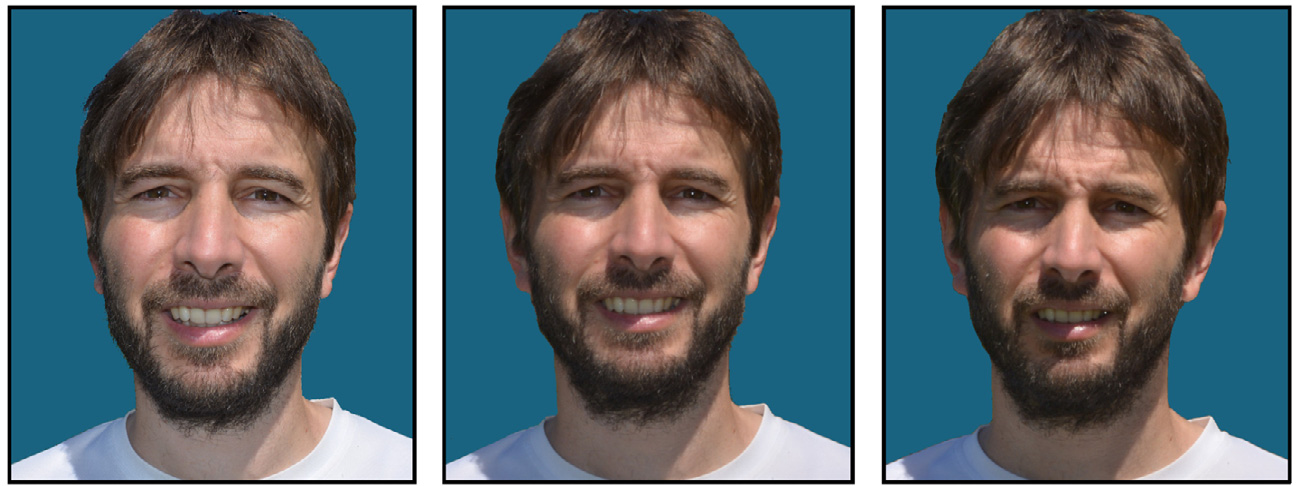
\includegraphics[scale=0.25]{imagenes/cap1/facial_distortion.png}
	\caption{Efectos de la distorsión de perspectiva en características faciales de fotografías realizadas a diferentes SCD: 0.5 m, 1 m y 3 m. Estos efectos varían en relación a la distancia y son independientes de la longitud focal~\cite{14}}
	\label{fig1}
\end{figure}

La estimación de la distancia entre la cámara y el sujeto en imágenes faciales permite cuantificar la cantidad de distorsión presente en una imagen, así como las diferencias en la distorsión entre dos conjuntos de imágenes.

%La estimación de la SCD en imágenes faciales abre la posibilidad a cuantificar las diferencias en la distorsión entre dos conjuntos de imágenes, y además, la posibilidad de reproducir las condiciones originales de la escena cuando hay disponibles modelos faciales 3D o restos esqueléticos. Esta última característica se considera esencial tanto para técnicas de identificación manual como automáticas, ya que mejoran la credibilidad de las comparaciones faciales mediante la medición y control de una mayor fuente de incertidumbre.

El único método totalmente automatizado para estimar la SCD en fotografías faciales, hasta la fecha, se conoce como FacialSCDnet~\cite{14}. Este método utiliza una arquitectura basada en aprendizaje profundo para procesar fotografías faciales y estimar la SCD con precisión.



Considerando todos estos aspectos, el presente Trabajo de Fin de Grado (TFG) consiste en mejorar el método actual del estado del arte en la estimación automática de la distancia cámara-sujeto en fotografías faciales mediante el uso de técnicas de aprendizaje profundo.


\section{Motivación}
En el ámbito forense, el principal foco recae sobre la determinación de la identidad humana cuando existe información esquelética~\cite{22}. En las últimas décadas, los antropólogos han centrado su atención en mejorar las técnicas para realizar una identificación más precisa. En este contexto, la estimación de la SCD juega un papel crucial, ya que, si estimamos la SCD con fiabilidad, podemos recrear la imagen con los restos esqueléticos (aplicando el valor de la SCD). A continuación, realizamos las comparaciones anatómicas mediante la superposición craneofacial~\cite{21} para identificar si se corresponde con la misma persona (ver Figura~\ref{fig2}). Si los parámetros de adquisición entre ambas imágenes (normal y esquelética) son distintos entonces dificultaría el análisis morfológico~\cite{23}.

\begin{figure}[h]
	\centering
	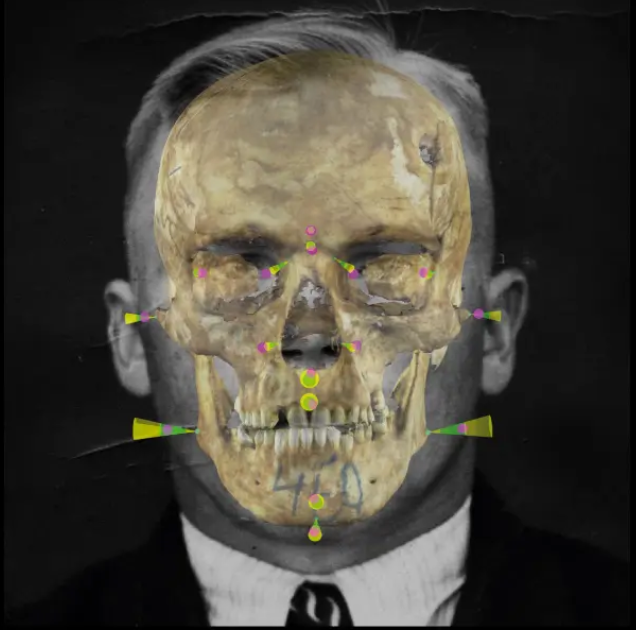
\includegraphics[scale=0.25]{imagenes/cap1/skull_superimposition.png}
	\caption{Ejemplo de superposición craneofacial~\cite{23}.}
	\label{fig2}
\end{figure}


Por otra parte, sabemos que la SCD y la distorsión de perspectiva (PD) tienen una relación de decremento logarítmico~\cite{23}. Esto significa que, para cuantificar el nivel de distorsión entre dos imágenes, bastaría con estimar la SCD para cada una de ellas, y mediante la siguiente fórmula hayamos el porcentaje de distorsión:

\[PD(\%) = (\frac{B'}{A'} - 1) \times 100\]

donde A' y B' son las proyecciones, en el sensor de la cámara, de los objetos A y B.

- Mitigar los efectos de la distorsión  DISCO


\section{Objetivos}
% Cambiar esto
%El objetivo general de este TFG consiste en mejorar el método actual del estado del arte en la estimación automática de la distancia cámara-sujeto en fotografías faciales.
 El objetivo general de este TFG consiste en desarrollar un modelo de aprendizaje profundo adecuado para mejorar la estimación de la distancia cámara-sujeto en fotografías faciales.Para el desarrollo del proyecto, dividiremos el objetivo general en una serie de objetivos parciales:
\begin{enumerate}
    \item Realizar un análisis exhaustivo del estado del arte para la estimación de la SCD en fotografías faciales.
    \item Generar un conjunto de datos sintético de mayor calidad (modelos 3D más completos de cuerpo entero y poses distintas, con fondos e iluminación más realistas)
    \item Realizar un estudio experimental que permita validar los enfoques propuestos y extraer conclusiones sobre su aplicabilidad al problema.
    \item Desarrollar y entrenar con nuevas arquitecturas que mejoren los resultados
    \item Usar tecnologías más recientes que mejoren los tiempos de aprendizaje y los resultados obtenidos
\end{enumerate}

\section{Planificación del proyecto}

Para abordar el desarrollo de este proyecto, es esencial considerar que el TFG tiene asignados 12 créditos ECTS, lo que equivale a aproximadamente 300 horas de trabajo. Dada la distribución temporal del segundo cuatrimestre, con unas 20 semanas disponibles, se estima que se requerirá dedicar al TFG unas 20 horas semanales, equivalentes a 4 horas diarias durante 5 días a la semana. Se reservan así 4 semanas como margen para posibles retrasos o imprevistos que puedan surgir durante el desarrollo del proyecto.

En cuanto a la metodología de desarrollo, se ha optado por seguir un enfoque basado en el ciclo de vida en cascada~\cite{38}, aunque con una variante que permite retroalimentación. Aunque el proyecto presenta requisitos y objetivos claros, se reconoce la posibilidad de ajustes menores durante su desarrollo, especialmente a medida que se obtenga más información sobre el problema y los métodos. Esta flexibilidad se considera crucial para adaptarse a posibles cambios en el contexto o los requisitos del proyecto.

Las fases del ciclo de vida del proyecto son las siguientes:

A continuación se describen las fases del ciclo de vida del proyecto:
\begin{itemize}
	\item Análisis de Requisitos: Consiste en las reuniones iniciales con los clientes, en este caso los directores del TFG. Se realiza un análisis del problema y un estudio detallado de la bibliografía existente
	\item Diseño: Consiste en la exploración y selección de los métodos apropiados basados en el análisis previo, tanto para la resolución como para la validación de la solución propuesta. Además, se llevarán a cabo pruebas preliminares y se elaborará el diseño del software experimental.
	\item Implementación: Consiste en la adaptación del código de los modelos investigados, la implementación de nuevas funcionalidades y la generación de un conjunto de datos sintético junto con su posterior preprocesado.
	\item Pruebas: Consiste en la realización de diversos experimentos para validar el funcionamiento del software desarrollado, utilizando los modelos y datos previamente definidos.
\end{itemize}

\begin{table}[htbp]
	\resizebox{\textwidth}{!}{%
	\begin{tabular}{|c|c|*{4}{c}|*{4}{c}|*{5}{c}|*{4}{c}|*{3}{c}|}
	\hline
	\rowcolor[HTML]{FFC702} 
	\cellcolor[HTML]{FFC702} & \cellcolor[HTML]{FFC702} & \multicolumn{4}{c|}{\cellcolor[HTML]{FFC702}Febrero} & \multicolumn{4}{c|}{\cellcolor[HTML]{FFC702}Marzo} & \multicolumn{5}{c|}{\cellcolor[HTML]{FFC702}Abril} & \multicolumn{4}{c|}{\cellcolor[HTML]{FFC702}Mayo} & \multicolumn{3}{c|}{\cellcolor[HTML]{FFC702}Junio} \\
	\rowcolor[HTML]{FFC702} 
	\multirow{-2}{*}{\cellcolor[HTML]{FFC702}Tarea} & \multirow{-2}{*}{\cellcolor[HTML]{FFC702}\begin{tabular}[c]{@{}c@{}}Semanas\\ - Horas\end{tabular}} & 5 & 12 & 19 & 26 & 4 & 11 & 18 & 25 & 1 & 8 & 15 & 22 & 29 & 6 & 13 & 20 & 27 & 3 & 10 & 17 \\ \hline
	Análisis de Requisitos & 3 - 60 & \cellcolor[HTML]{9B9B9B} & \cellcolor[HTML]{9B9B9B} & \cellcolor[HTML]{9B9B9B} &  &  &  &  &  &  &  &  &  &  &  &  &  &  &  &  &  \\ \cline{1-1}
	Diseño & 3 - 60 &  &  &  & \cellcolor[HTML]{9B9B9B}{\color[HTML]{C0C0C0} } & \cellcolor[HTML]{9B9B9B}{\color[HTML]{C0C0C0} } & \cellcolor[HTML]{9B9B9B}{\color[HTML]{C0C0C0} } &  &  &  &  &  &  &  &  &  &  &  &  &  &  \\ \cline{1-1}
	Implementación & 5 - 90 &  &  &  &  &  &  & \cellcolor[HTML]{9B9B9B} & \cellcolor[HTML]{9B9B9B} & \cellcolor[HTML]{9B9B9B} & \cellcolor[HTML]{9B9B9B} & \cellcolor[HTML]{9B9B9B} &  &  &  &  &  &  &  &  &  \\ \cline{1-1}
	Pruebas & 5 - 90 &  &  &  &  &  &  &  &  &  &  &  & \cellcolor[HTML]{9B9B9B} & \cellcolor[HTML]{9B9B9B} & \cellcolor[HTML]{9B9B9B} & \cellcolor[HTML]{9B9B9B} & \cellcolor[HTML]{9B9B9B} &  &  &  &  \\ \hline
	\end{tabular}%
	}
	\caption{Planificación inicial del proyecto}
	\label{planif-ini}
\end{table}

\chapter{Fundamentos teóricos}
\thispagestyle{empty}

\section{Aprendizaje automático}
El aprendizaje automático (\textit{Machine Learning}, ML) \cite{22,23} es una rama de la inteligencia artificial y de las ciencias de la computación centrada en el uso de datos y algoritmos para imitar la forma en la que los humanos aprenden, detectando patrones o regularidades para realizar predicciones.

Existen 3 tipos de aprendizaje dentro del ML:

El \textbf{aprendizaje supervisado} consiste en entrenar un modelo con datos que tienen etiquetas conocidas, lo que indica la categoría a la que pertenece cada dato. Por ejemplo, si los datos de entrada son imágenes de animales, las etiquetas podrían ser \enquote*{perro} o \enquote*{gato}. A partir de estos datos etiquetados, el modelo aprende a predecir la etiqueta de nuevos datos. Es el tipo de aprendizaje más utilizado y los datos vienen ya \enquote*{preparados} para su uso. Es el tipo de aprendizaje que utilizaremos en este TFG.

En el \textbf{aprendizaje no supervisado}, el modelo analiza los datos de entrada sin etiquetas, buscando patrones y estructuras inherentes a los datos. El agrupamiento es una técnica común en este tipo de aprendizaje, ya que identifica posibles grupos dentro de los datos. Este enfoque suele requerir un gran volumen de datos para ser efectivo.

Por otro lado, en el \textbf{aprendizaje por refuerzo}, el modelo aprende a través de recompensas o penalizaciones en función de las acciones que realiza. El objetivo del agente es maximizar las recompensas a largo plazo, lo que lo hace especialmente útil en la enseñanza de estrategias en juegos y otras interacciones dinámicas.

\section{Aprendizaje profundo}

\subsection{Redes neuronales artificiales}
Las redes neuronales artificiales (\textit{Artificial Neural Networks}, ANN) \cite{24, 25, 27} son redes computacionales que intentan, a groso modo, simular el proceso de decisión de las neuronas del sistema nervioso central de animales y humano. Las ANN poseen unidades de procesamiento de información llamadas neuronas, las cuales están conectadas entre sí. La estructura básica de una ANN se compone de (ver Figura \ref{fig4}):
\begin{itemize}
	\item Una capa de entrada, que tendrá tantos \textit{inputs} como características o variables tenga el problema
	\item Una o varias capas ocultas, compuestas por neuronas. El número de capas ocultas define la profundidad de la red neuronal.
	\item Una capa de salida, la cual representa el valor o valores predichos
\end{itemize} 

\begin{figure}[h]
	\centering
	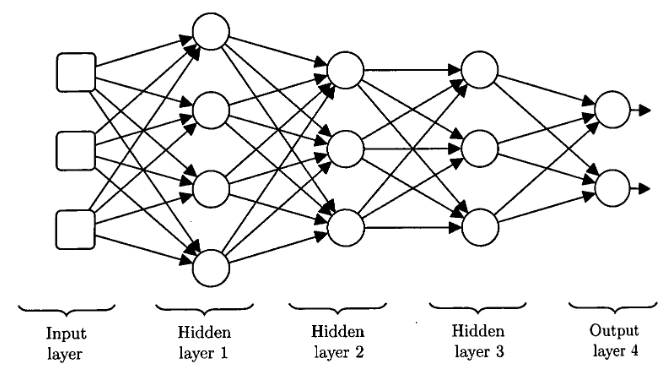
\includegraphics[scale=0.5]{imagenes/cap2/neural-network.png}
	\caption[Esquema de red neuronal.]{Esquema de una red neuronal \cite{26}.}
	\label{fig4}
\end{figure}

Las neuronas son la unidad fundamental de cómputo, tienen varios valores de entrada y un valor de salida que se conecta con las neuronas de la siguiente capa. Los elementos básicos del modelo neuronal son (ver Figura \ref{fig5}):

\begin{itemize}
	\item Un conjunto de conexiones con las señales de entrada. Cada conexión tiene su propio peso/fuerza.
	\item Una función de suma de las señales de entrada, ponderadas cada una con su peso. Estas operaciones constituyen una combinación lineal.
	\item Una función de activación, para limitar la amplitud de la salida de la neurona. Normalmente, el rango de salida está en el intervalo [0,1], o alternativamente en [-1,1]. Existen muchos tipos de funciones de activación pero, se suelen utilizar cuatro: la función signo, la función logística, la función arco-tangente o la función ReLU (\textit{Rectified Linear Unit}).
\end{itemize} 

\begin{figure}[h]
	\centering
	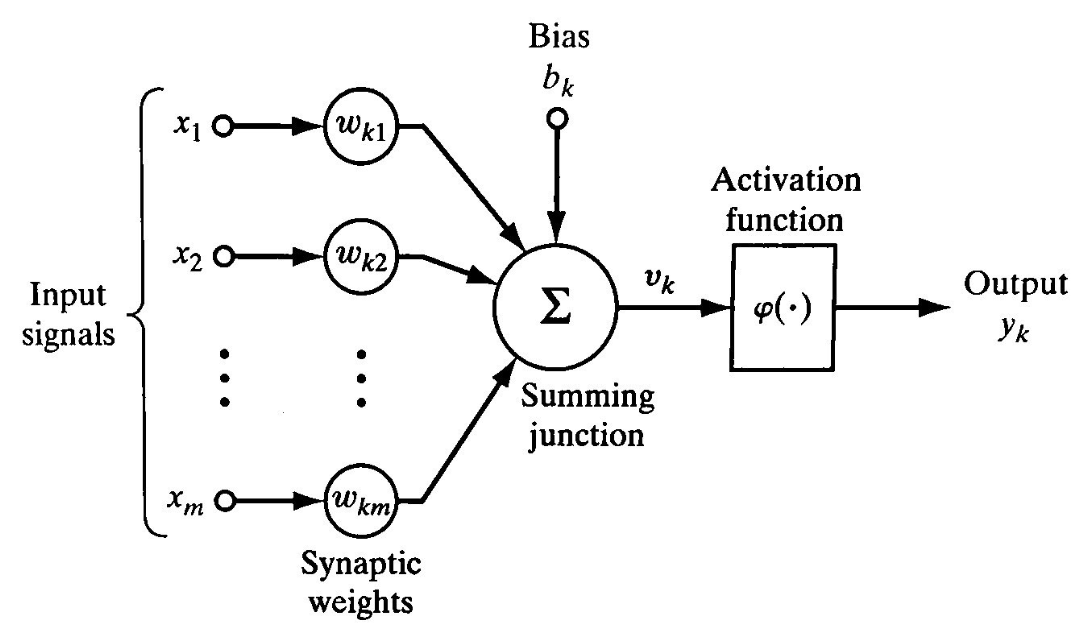
\includegraphics[scale=0.25]{imagenes/cap2/neuron-model.png}
	\caption[Modelo neuronal.]{Modelo neuronal para una neurona $k$ \cite{25}.}
	\label{fig5}
\end{figure}

En términos matemáticos, podemos describir la salida de una neurona como:

\begin{equation}
	y = \phi(\sum_{j=1}^{m} w_j x_j + b)
\end{equation}

siendo $\phi$ la función de activación, $m$ el número de señales de entrada, $w_j$ el peso de cada entrada $x_j$, y $b$ el sesgo.

El algoritmo de aprendizaje de la red neuronal consiste en ir modificando los pesos y el sesgo, iterativamente, hasta alcanzar el resultado deseado. Este proceso iterativo se conoce como entrenamiento, y permite, a través de las modificaciones de los pesos, reconocer y extraer las características más relevantes de los datos.

El objetivo del entrenamiento es minimizar el error de predicción de la salida de la red neuronal, para ello, se define una función de pérdida. Existen numerosas funciones de pérdida, algunas de las más conocidas son: el error cuadrático medio (MSE), el error absoluto medio (MAE) o la entropía cruzada. La información de la función de pérdida se transmite desde la salida a la capa inicial, con el fin de modificar adecuadamente los pesos para generar una mejor estimación de la predicción.

Uno de los aspectos más importantes al entrenar un modelo es el sobreajuste. Este fenómeno ocurre cuando el modelo se adapta excesivamente al conjunto de datos de entrenamiento, lo que resulta en un rendimiento deficiente al enfrentarse a nuevos datos no incluidos en el entrenamiento. Esto se debe a una limitada capacidad de generalización, que puede mitigarse mediante técnicas de regularización \ref{regularizacion}.


\subsection{Redes neuronales convolucionales}
Las redes neuronales convolucionales (\textit{Convolutional Neural Networks}, CNN) \cite{35, 36, 37} son un tipo de red neuronal profunda que trabaja con patrones de cuadrícula, como pueden ser imágenes (ver Figura \ref{fig6}).

En estas redes neuronales, las capas convolucionales desempeñan un papel fundamental, y a menudo se complementan con capas de \textit{pooling}. Dichas capas se encuentran en la primera parte de la red y son las encargadas de extraer las características relevantes de la entrada. Esto posibilita la automatización del proceso de extracción de características, mejorando simultáneamente tanto el tiempo como el rendimiento.

\begin{figure}[h]
	\centering
	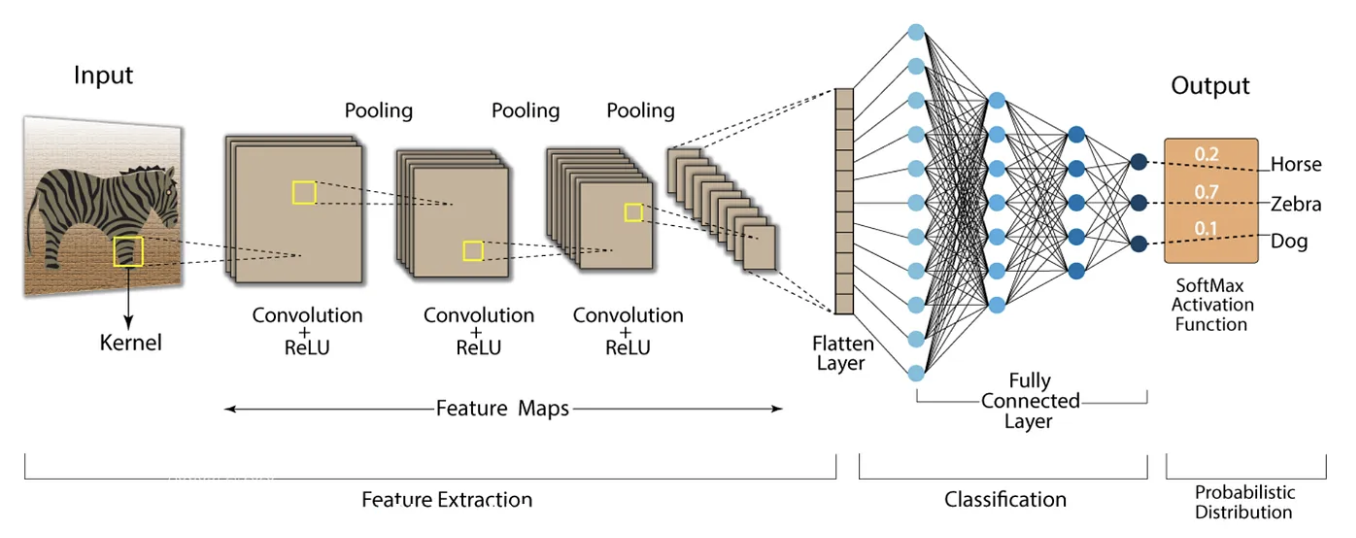
\includegraphics[scale=0.5]{imagenes/cap2/cnn.png}
	\caption[Ejemplo de red neuronal convolucional.]{Ejemplo de red neuronal convolucional \cite{41}.}
	\label{fig6}
\end{figure}

A continuación, se describen los posibles tipos de capas presentes en una CNN \cite{39,40}:


\subsubsection*{Capa de convolución}

La capa convolucional es un componente fundamental de las CNN, utilizada para la extracción de características de una imagen o un conjunto de imágenes. Esta capa aplica una operación lineal especializada conocida como convolución, que consiste en aplicar un filtro o \textit{kernel} a la imagen de entrada. El \textit{kernel} es una matriz que se desliza a lo largo de la imagen, multiplicando sus valores con los píxeles correspondientes y sumándolos para producir un único valor en la imagen de salida. Este proceso se repite en todas las posiciones de la imagen dando como resultado una nueva matriz denominada mapa de características (ver Figura \ref{fig7}).

\begin{figure}[h]
	\centering
	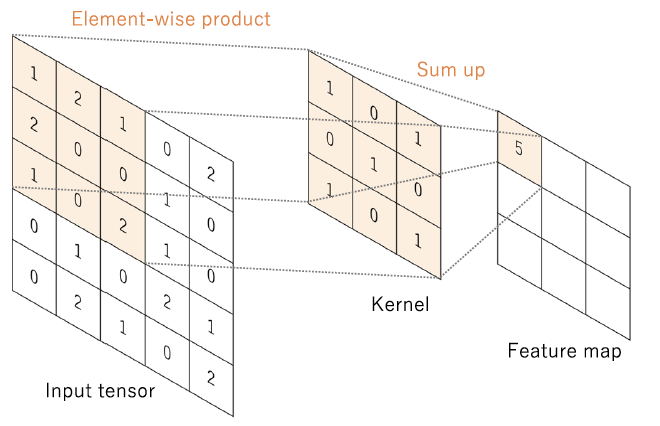
\includegraphics[scale=0.75]{imagenes/cap2/convolution.png}
	\caption[Ejemplo de operación de convolución.]{Ejemplo de operación de convolución en CNN \cite{40}.}
	\label{fig7}
\end{figure}

Los pesos de los filtros se aprenden durante el proceso de entrenamiento de la red neuronal. Cada \textit{kernel} tiene sus propios pesos que se ajustan iterativamente durante el entrenamiento para minimizar la función de pérdida y mejorar el rendimiento del modelo.

La característica clave de la operación de convolución es el \textit{weight sharing}, que implica compartir los mismos \textit{kernels} en toda la imagen. Esto permite que la red detecte patrones locales independientemente de su ubicación en la imagen. Además, contribuye a aprender jerarquías de características espaciales, lo que permite capturar una amplia gama de características en varios niveles de abstracción. Este enfoque también aumenta la eficiencia del modelo al reducir la cantidad de parámetros que necesita aprender en comparación con las redes totalmente conectadas.

Por otro lado, es importante la configuración de los hiperparámetros de cada capa convolucional, estos se definen antes de iniciar el entrenamiento de la red neuronal y afectan al comportamiento de la misma. Los más comunes son:
\begin{itemize}
	\item Tamaño del \textit{kernel}: se refiere a las dimensiones del filtro que se aplica a la imagen de entrada. Los tamaños comunes son 3x3, 5x5 o 7x7.
	\item Número de \textit{kernels}: indica cuántos filtros se aplicarán a la imagen de entrada para extraer diferentes características. Cuantos más \textit{kernels} se utilicen, mayor será la profundidad de los mapas de características de salida.
	\item \textit{Padding}: esta técnica consiste en añadir píxeles alrededor de la imagen de entrada tras el proceso de convolución. Su propósito es mantener el tamaño de la salida, ya que al aplicar la convolución, las dimensiones del mapa de características se reducen con respecto a la imagen original.
	\item \textit{Stride}: es el número de píxeles que se desplaza el \textit{kernel} en cada paso durante la convolución. Un mayor \textit{stride} reduce el tamaño del mapa de características y la cantidad de operaciones necesarias.
\end{itemize}

Sin embargo, es importante tener en cuenta que la operación de convolución por sí sola es lineal y puede no ser suficiente para aprender patrones complejos. En este contexto, entra en juego la capa de activación, que introduce no linealidades en la red y potencia su capacidad para capturar relaciones más complejas entre las características extraídas.

\subsubsection*{Capa de activación}

La capa de activación en una CNN sigue a la capa convolucional y se encarga de introducir no linealidades en el modelo mediante una función de activación.
Esta función aumenta la capacidad de la red para aprender relaciones no lineales en los datos, lo que es fundamental para capturar patrones más complejos. Algunas de las funciones de activación comunes utilizadas son la función ReLU, la función sigmoide y la función tangente hiperbólica (ver Figura \ref{fig8}).

\begin{figure}[h]
	\centering
	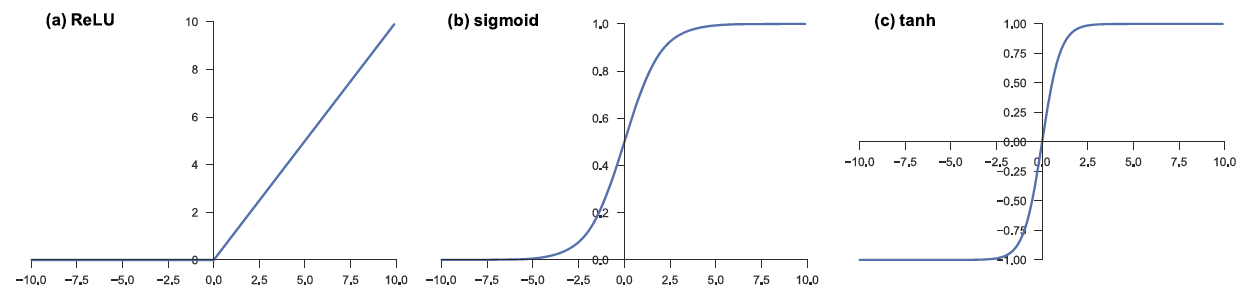
\includegraphics[scale=0.55]{imagenes/cap2/activation.png}
	\caption[Funciones de activación comunes.]{Funciones de activación comúnmente aplicadas en CNN \cite{40}.}
	\label{fig8}
\end{figure}

\subsubsection*{Capa de \textit{pooling}}
La capa de \textit{pooling} también es específica de las CNN y se encarga de reducir la dimensionalidad de las características conservando la información más relevante.

Esta capa resume la información en regiones locales mediante una operación de \textit{downsampling} en las características de entrada. Al reducir la dimensionalidad de las características, la capa de \textit{pooling} disminuye el número de parámetros aprendibles en la red, lo que puede ayudar a prevenir el sobreajuste y mejorar la eficiencia computacional del modelo. Además, esta capa también ayuda a introducir invariancia a pequeñas traslaciones y distorsiones en los datos de entrada, permititiendo a la red reconocer patrones incluso si están ligeramente desplazados en la imagen. 

Los dos tipos más comunes de \textit{pooling} son el \textit{max pooling}, que selecciona el valor máximo de una región local en las características de entrada, y el \textit{average pooling}, que calcula el promedio de los valores en una región local (ver Figura \ref{fig9}).

\begin{figure}[h]
	\centering
	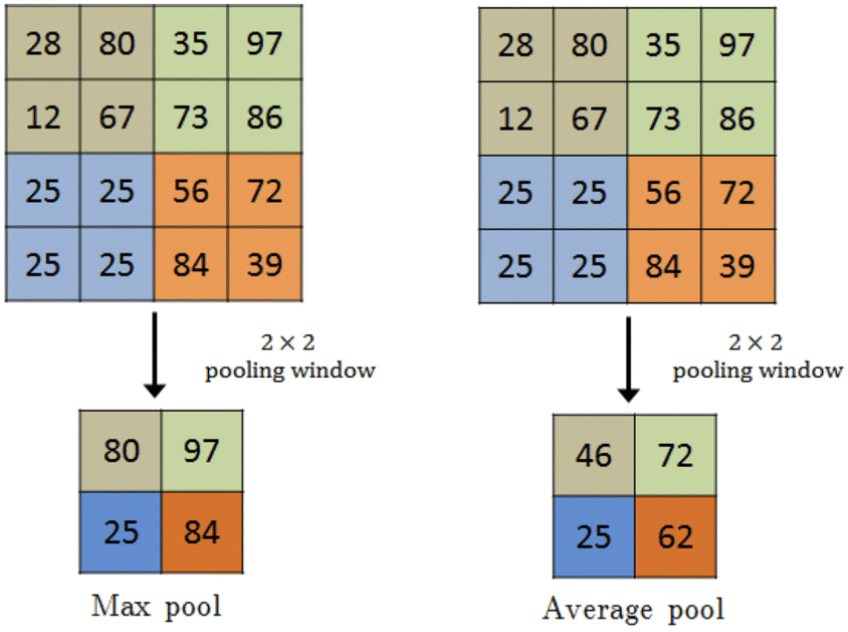
\includegraphics[scale=0.55]{imagenes/cap2/pooling.png}
	\caption[Tipos de \textit{pooling} comunes.]{Tipos de \textit{pooling} comúnmente utilizados en CNN \cite{42}.}
	\label{fig9}
\end{figure}

Los hiperparámetros de la capa de \textit{pooling} incluyen el tamaño del filtro, el \textit{stride} y el tipo de \textit{padding}. Estos hiperparámetros afectan la forma en que se realiza el \textit{downsampling} en las características.

\subsubsection*{Capa totalmente conectada}

La capa totalmente conectada sigue a las capas de convolución y \textit{pooling}. En esta capa, las características extraídas por las capas anteriores se transforman en un formato unidimensional (vector) antes de conectarse a una o más capas totalmente conectadas, también conocidas como capas densas.

Esta capa, al igual que en las redes neuronales clásicas, tiene la responsabilidad de combinar y procesar las características extraídas para producir la salida final de la red.

Cada neurona en una capa totalmente conectada está conectada a todas las neuronas de la capa anterior a través de pesos aprendibles. Estos pesos determinan la contribución de cada neurona de entrada a la neurona de salida correspondiente en la capa totalmente conectada. Durante el entrenamiento, estos pesos se ajustan mediante algoritmos de optimización como \textit{backpropagation} y descenso de gradiente para minimizar la diferencia entre las salidas predichas y las etiquetas reales.

Es importante destacar que la capa totalmente conectada suele estar seguida por una función de activación no lineal, como ReLU, para introducir no linealidades en el modelo y permitir la representación de patrones complejos en los datos. Además, la última capa de activación de la CNN, generalmente se selecciona según la naturaleza de la tarea que se está abordando.

\subsection{Transferencia de aprendizaje}

La transferencia de aprendizaje \cite{49}, también conocida como \textit{Transfer Learning} (TL), es una técnica fundamental en el campo del aprendizaje automático. Consiste en aprovechar el conocimiento adquirido al resolver un problema para mejorar el rendimiento en otro problema relacionado. En lugar de comenzar desde cero al entrenar un modelo para una tarea específica, el TL utiliza el aprendizaje previo en tareas similares, obteniendo múltiples beneficios, como una mayor eficiencia en el entrenamiento de modelos, una mejor generalización con conjuntos de datos limitados y una aceleración en el desarrollo de modelos.

En las arquitecturas convolucionales, la forma más común de llevar a cabo la transferencia de aprendizaje es mediante el \textit{fine-tuning} \cite{39}, que implica utilizar pesos pre-entrenados, congelar todas las capas de la red excepto las superiores, y ajustar estas últimas para adaptarlas a nuestro problema específico, de manera que el entrenamiento se realice únicamente en esas capas superiores. Este enfoque aprovecha la capacidad de los modelos pre-entrenados para capturar características generales de los datos, lo cual es especialmente útil cuando se dispone de conjuntos de datos pequeños o limitados. Además, al congelar las capas iniciales se evita la pérdida de información importante aprendida durante el pre-entrenamiento, mientras que el \textit{fine-tuning} en las capas superiores permite adaptar el modelo a la nueva tarea específica.

En este contexto, es común utilizar los pesos pre-entrenados en el conjunto de datos de ImageNet \cite{50} debido a su gran tamaño, diversidad, representatividad y disponibilidad.


\subsection{Regularización}\label{regularizacion}
Tanto en las redes neuronales clásicas como en las convolucionales, el sobreajuste a los datos de entrenamiento es una problema importante (ver Figura \ref{fig10}). Aunque la solución óptima sería adquirir más datos para el entrenamiento, esta opción no siempre está disponible. Por tanto, se recurre a técnicas de regularización para mitigar este problema. Entre las más destacadas se encuentran:

\begin{itemize}
	\item \textit{Dropout}: es una técnica de regularización donde se establecen aleatoriamente ciertas activaciones a 0 durante el entrenamiento, de modo que el modelo se vuelve menos sensible a pesos específicos en la red.
	\item \textit{Weight decay}: también conocido como regularización L2, reduce el sobreajuste penalizando los pesos del modelo para que tomen solo valores pequeños.
	\item \textit{Batch normalization}: es un tipo de capa suplementaria que normaliza adaptativamente los valores de entrada de la siguiente capa, mitigando el riesgo de sobreajuste, así como mejorando el flujo de gradiente a través de la red, permitiendo tasas de aprendizaje más altas y reduciendo la dependencia de la inicialización.
	\item \textit{Data augmentation}: es un proceso de modificación de los datos de entrenamiento a través de transformaciones aleatorias, como volteo, traslación, recorte, rotación y borrado aleatorio, para que el modelo no vea exactamente las mismas entradas durante las iteraciones de entrenamiento. Esta técnica, además de reducir el sobreajuste, permite una mejor generalización del modelo.
	\item Elección del modelo: un modelo de una alta complejidad puede provocar sobreajuste ya que tiene la capacidad de ajustarse mucho mejor a los datos de entrenamiento. Es fundamental encontrar un modelo que tenga un equilibrio entre complejidad y generalización, es decir, que sea lo suficientemente complejo para captar las características importantes pero que a la vez sea capaz de generalizar sin sobreajustarse demasiado a los datos.
\end{itemize}

\begin{figure}[h]
	\centering
	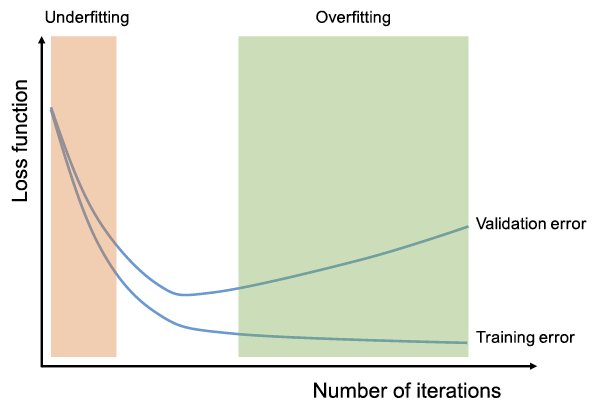
\includegraphics[scale=0.8]{imagenes/cap2/sobreajuste.png}
	\caption[Infraajuste y sobreajuste en entrenamiento.]{Zona de infraajuste y sobreajuste durante el entrenamiento \cite{40}.}
	\label{fig10}
\end{figure}

A pesar de las técnicas anteriores, persiste la preocupación por el sobreajuste al conjunto de validación en lugar del conjunto de entrenamiento, principalmente debido a la filtración de información durante el ajuste fino de hiperparámetros y el proceso de selección del modelo. Por tanto, es importante evaluar el rendimiento del modelo final en un conjunto de prueba separado, preferiblemente no visto previamente. Esto es fundamental para validar la capacidad de generalización del modelo y garantizar su fiabilidad.


\section{Parámetros de la cámara}

A la hora de trabajar con imágenes faciales y, particularmente, para comprender todos los factores que intervienen en el proceso de la simulación de imágenes faciales, es esencial introducir una serie de conceptos relativos a los parámetros de la cámara \cite{51,67,68,69}. Estos parámetros, como la longitud focal, el sensor de la cámara y la distancia cámara-sujeto, entre otros, están estrechamente relacionados entre sí y ejercen una influencia significativa tanto en la configuración de la escena fotográfica como en la percepción visual de los sujetos retratados en ella.

\subsection*{Longitud focal}
La longitud focal mide la distancia, en milímetros, entre el \textit{punto nodal} (punto donde la luz converge en una lente) y el sensor de la cámara (ver Figura \ref{fig11}). 

\begin{figure}[h]
	\centering
	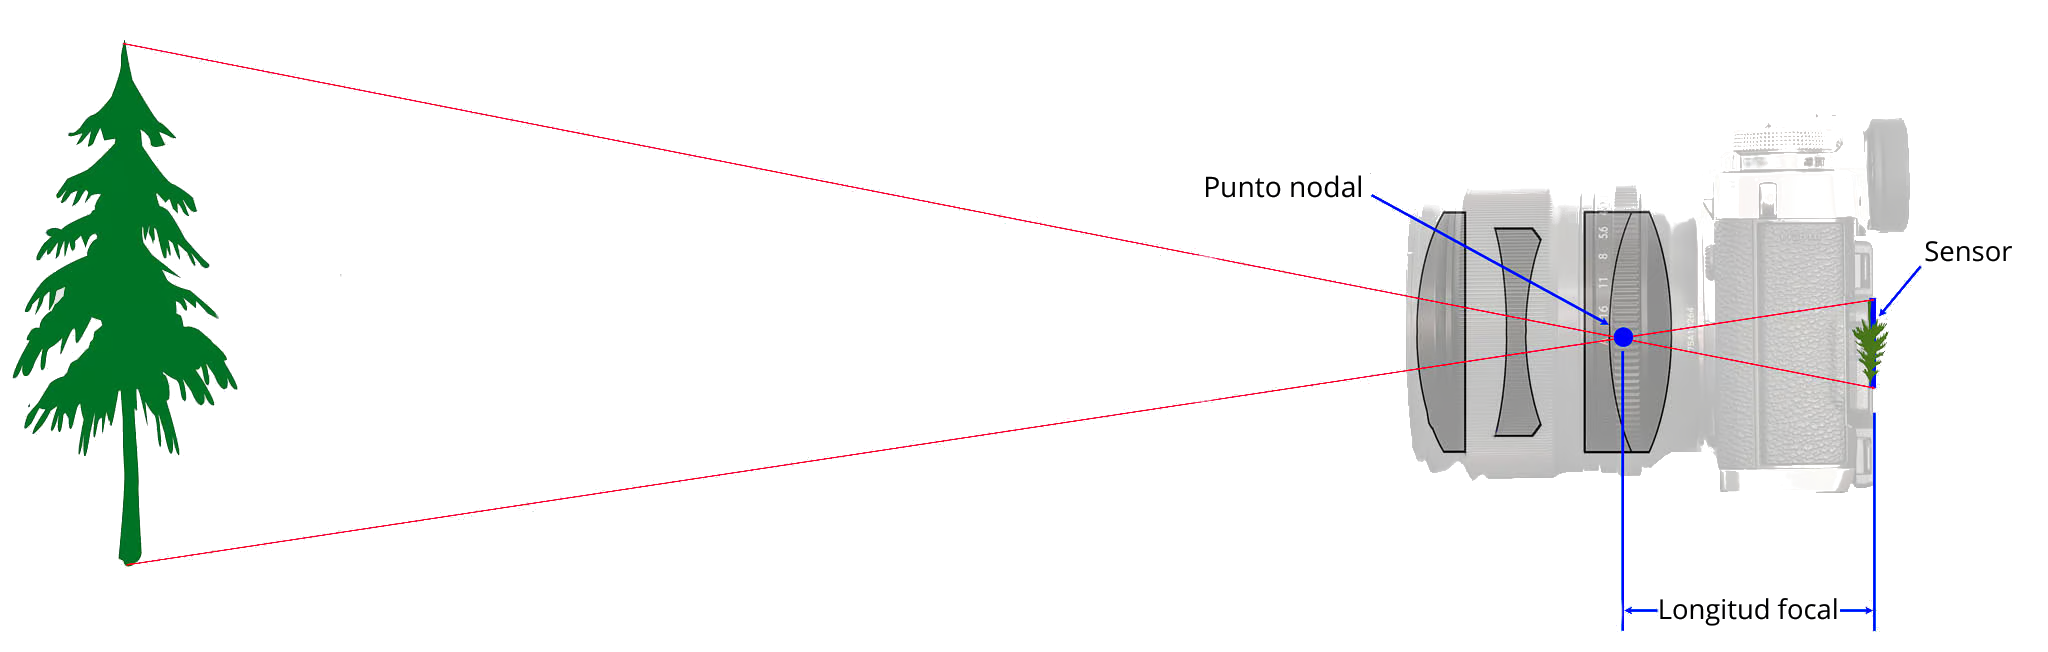
\includegraphics[scale=0.2]{imagenes/cap2/focal.png}
	\caption[Relación entre punto nodal y longitud focal.]{Relación entre punto nodal y longitud focal \cite{44}}
	\label{fig11}
\end{figure}

La longitud focal es un factor importante, ya que determina el campo de visión de una lente, es decir, la cantidad de escena que se captura (ver Figura \ref{fig11.2}).  En longitudes focales más largas, los objetos parecen estar más cerca del objetivo de la cámara, lo que puede hacer que parezcan más grandes en la imagen. Por el contrario, con longitudes focales más cortas, los objetos aparentan estar más distantes en la fotografía.

\begin{figure}[h]
	\centering
	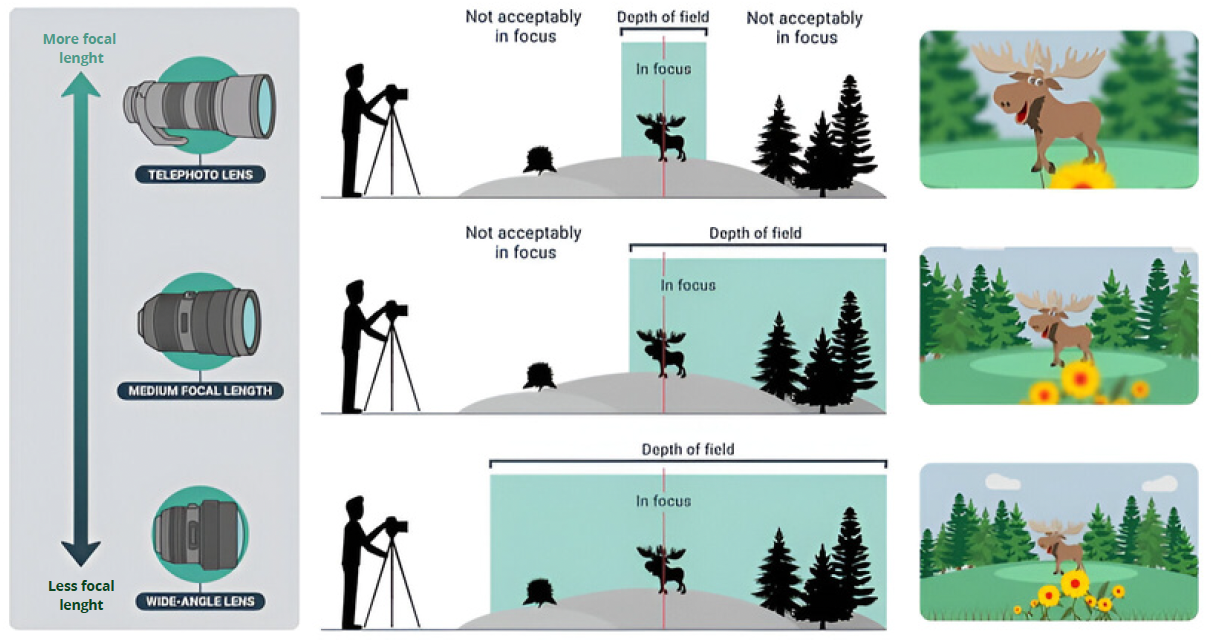
\includegraphics[scale=0.55]{imagenes/cap1/perspective.png}
	\caption[Relación entre longitud focal y campo de visión.]{Relación entre longitud focal y campo de visión. La longitud focal afecta al tamaño aparente de los objetos y a la cantidad de escena que aparece en la imagen.}
	\label{fig11.2}
\end{figure}

\subsection*{Sensor de la cámara}
El sensor de la cámara es el componente encargado de capturar la luz y transformarla en una imagen digital. Su tamaño incide directamente en la calidad de la imagen y en su capacidad para capturar la luz. El estándar comúnmente utilizado es de 36mm x 24mm, conocido como \textit{full frame} o 35mm, siendo este tamaño una referencia debido a su similitud con el formato de película fotográfica analógica utilizado en el pasado.

La necesidad de establecer un estándar es esencial para comparar equitativamente imágenes capturadas por diferentes dispositivos. Al referirnos a un estándar de 35 mm, disponemos de un sistema de referencia común que nos permite convertir las imágenes, de manera que los objetos visibles en la escena tengan dimensiones similares, facilitando así su comparación y análisis.

Otra manera de expresar el tamaño del sensor es a través del factor de recorte, que se calcula como la proporción entre el tamaño del sensor de 35 mm y el de nuestra cámara (ver Figura \ref{fig12}). El factor de recorte se emplea a menudo para comprender la dimensión del sensor de la cámara en relación con el estándar de 35 mm. Esta medida facilita una comparación directa entre el tamaño del sensor de 35 mm y el de nuestra cámara, lo que permite entender mejor su capacidad para capturar imágenes.

\begin{figure}[h]
	\centering
	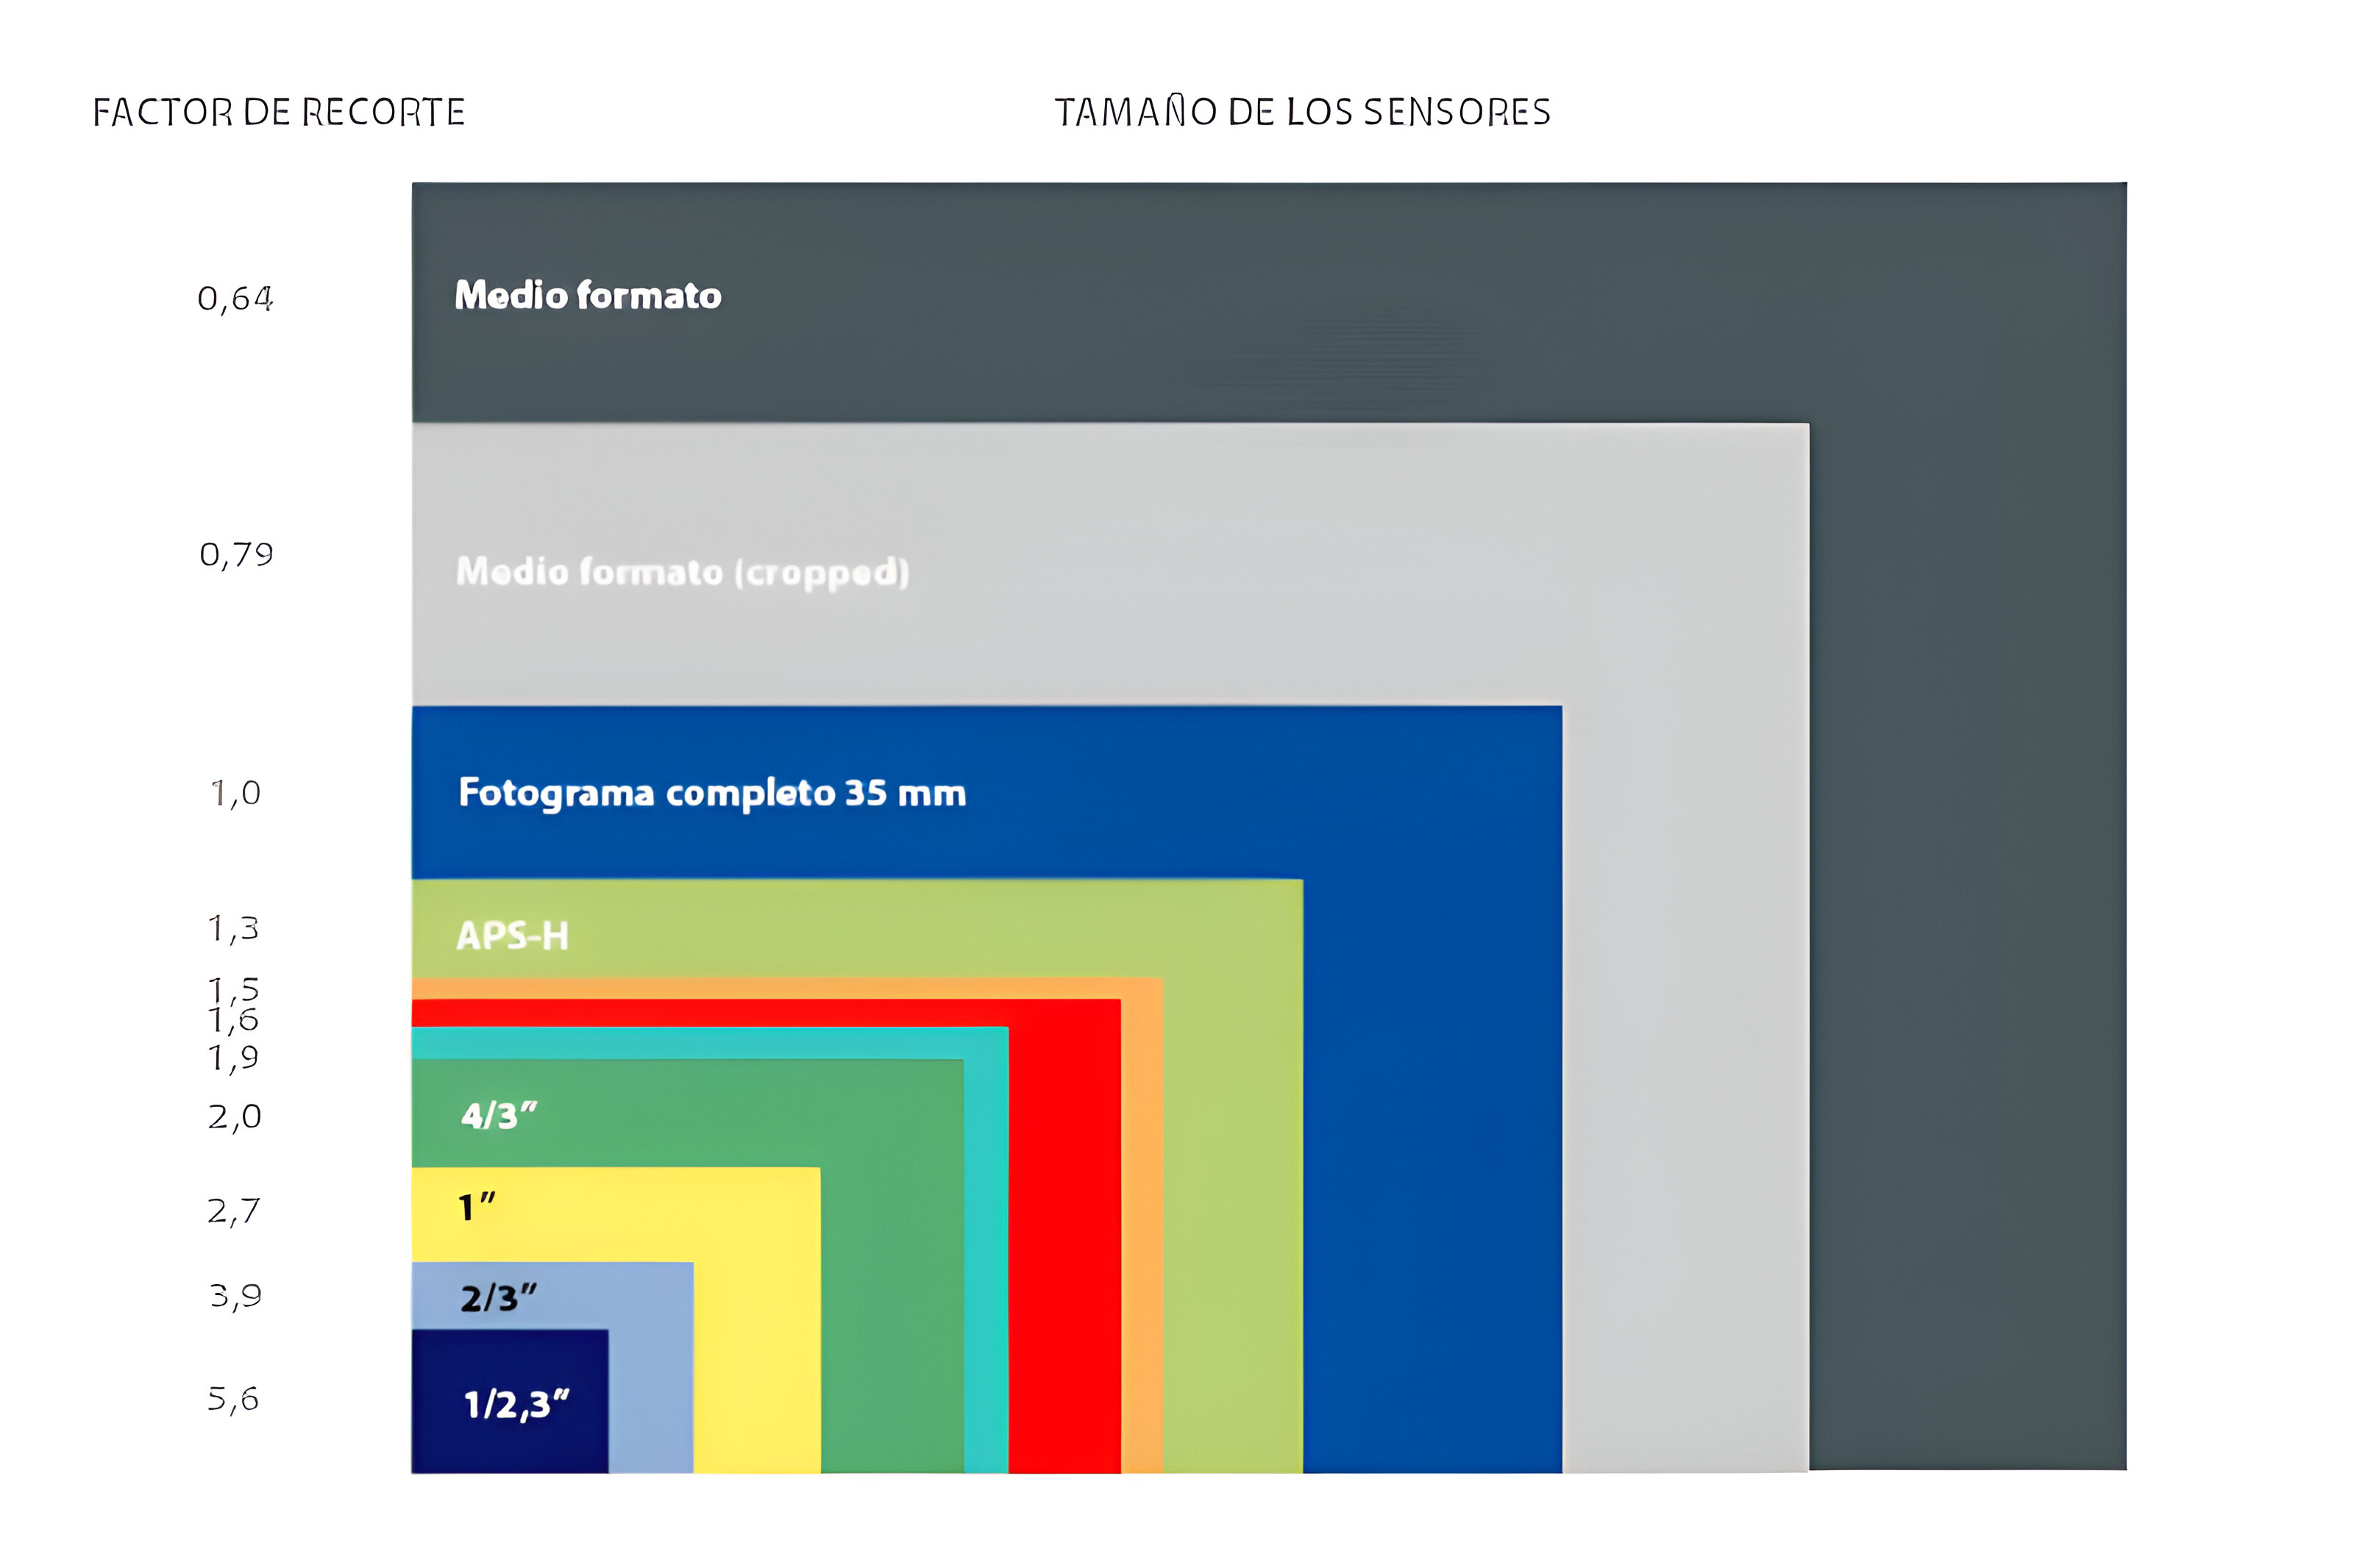
\includegraphics[scale=0.08]{imagenes/cap2/tam_sensor_factor.jpeg}
	\caption[Tipos de tamaños de sensor.]{Tamaños del sensor expresados según el factor de recorte \cite{48}}
	\label{fig12}
\end{figure}

Uno de los aspectos más importantes del factor de recorte es su impacto en la longitud focal, lo que nos lleva al concepto de \textit{longitud focal equivalente}. Por ejemplo, al tener una focal de 300 mm en un sensor con factor de recorte 1.6, estaríamos obteniendo un efecto equivalente al de una focal de 480 mm (300 mm x 1.6) en un sensor \textit{full frame} con factor de recorte 1.

\begin{figure}[h]
	\centering
	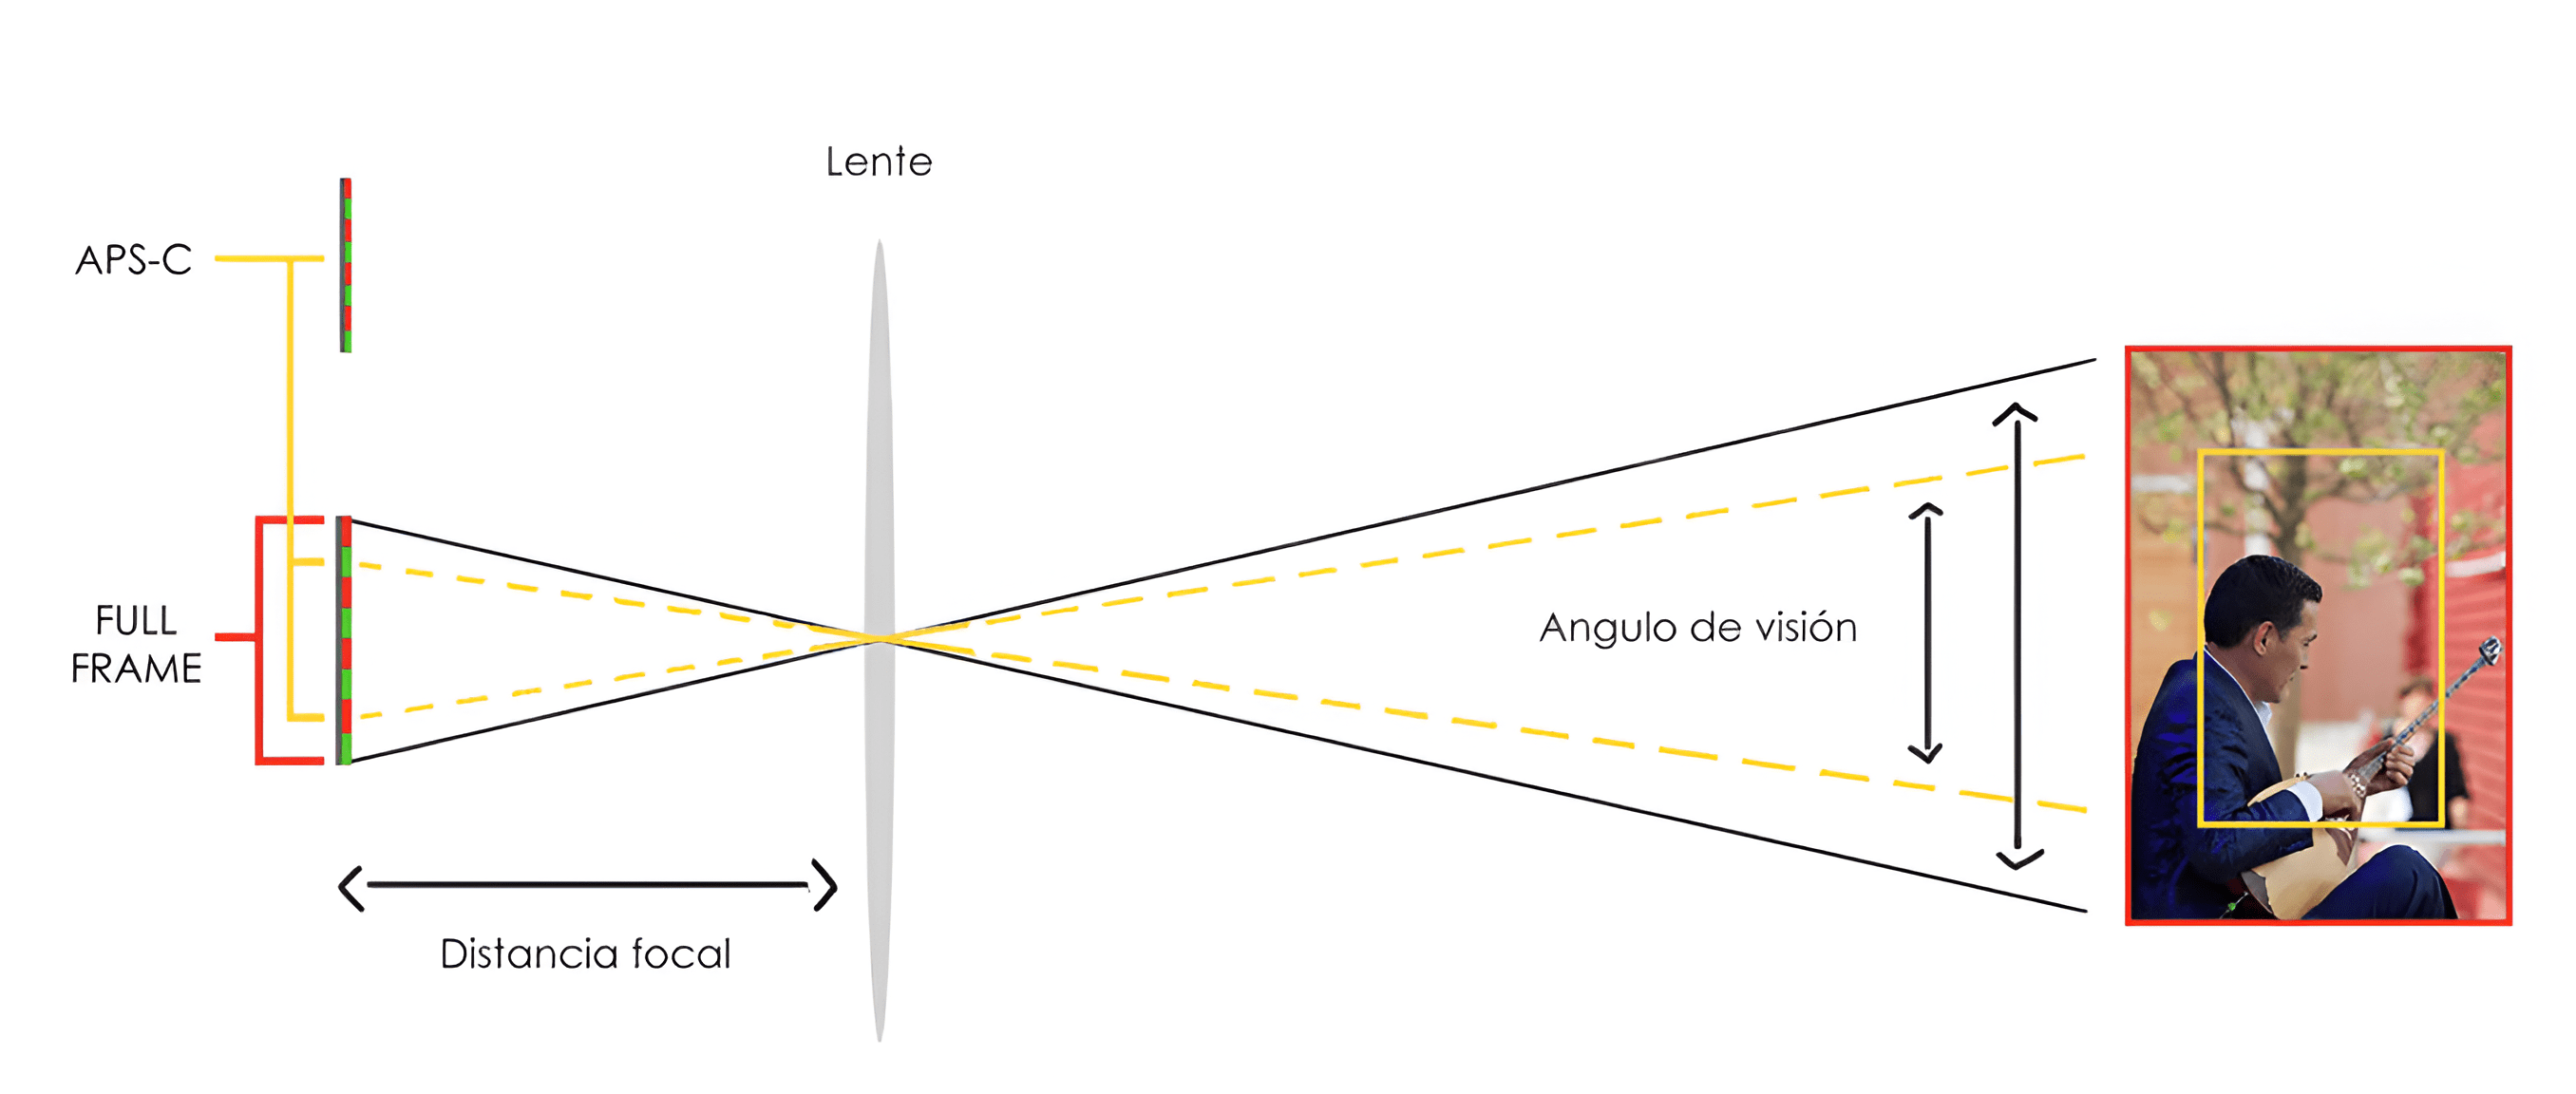
\includegraphics[scale=0.13]{imagenes/cap2/focal-equivalente.png}
	\caption[Ejemplo de longitud focal equivalente.]{Ejemplo de longitud focal equivalente según el tamaño del sensor \cite{46}.}
	\label{fig13}
\end{figure}


\subsection*{Distancia cámara-sujeto}

La distancia cámara-sujeto se define como la separación física entre la cámara y el sujeto que está siendo fotografiado (ver Figura \ref{fig14}). Modificar esta distancia provoca variaciones en la apariencia visual del rostro en la fotografía obtenida \cite{43}. Este fenómeno se conoce como distorsión de perspectiva.

\begin{figure}[h]
	\centering
	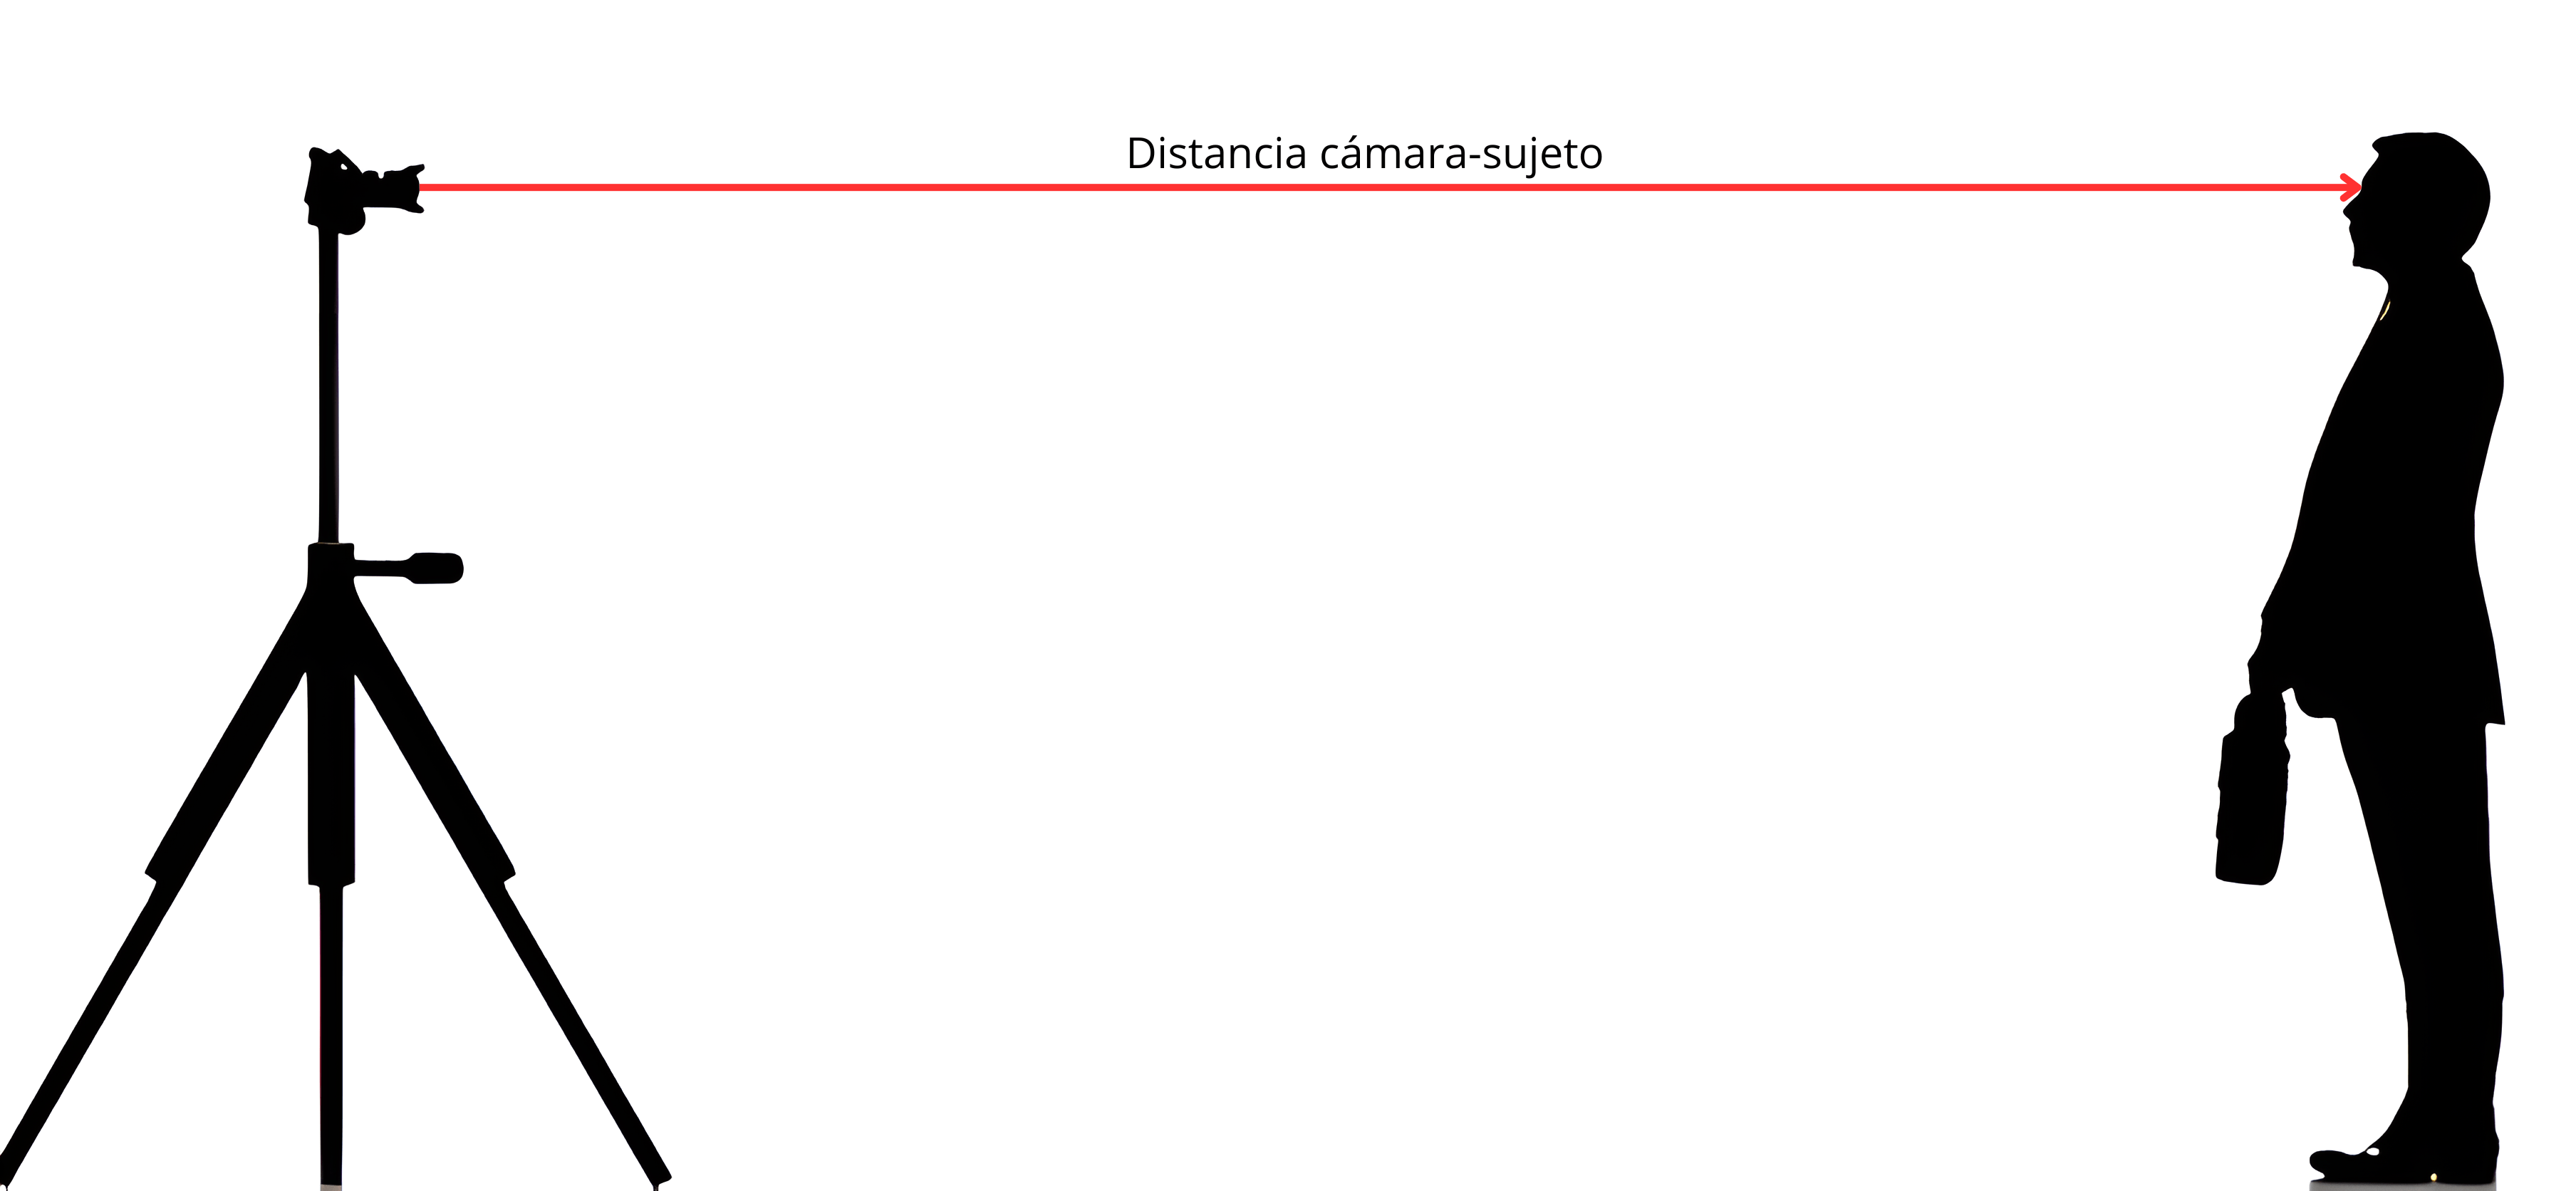
\includegraphics[scale=0.1]{imagenes/cap2/SCD_final.png}
	\caption[Distancia desde la cámara al sujeto.]{Distancia desde la cámara al sujeto.}
	\label{fig14}
\end{figure}

La distorsión de perspectiva \cite{8,51} es la transformación que sufre un objeto y su entorno debido a la proximidad del mismo respecto al objetivo (ver Figura \ref{fig15}). En el caso de las fotografías faciales, cuanto menor es la distancia cámara-sujeto, mayor es la distorsión de perspectiva que afecta a la persona fotografiada. Esto afecta a rasgos de la cara que pueden aparecer más grandes, como la nariz, o más pequeños, como las orejas, de lo que realmente son (ver Figura \ref{fig2}).

\begin{figure}[h]
	\centering
	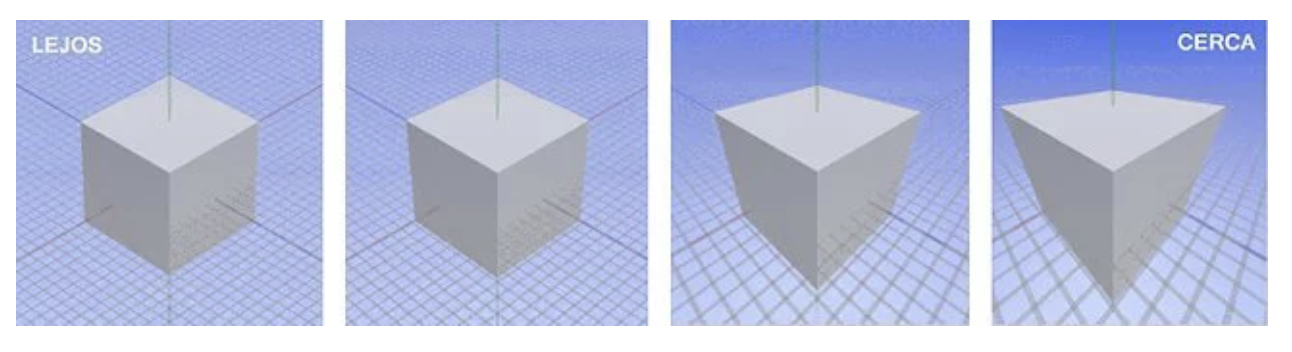
\includegraphics[scale=0.5]{imagenes/cap2/distorsion.png}
	\caption[Efectos de la distorsión según distancia.]{Efecto de la distorsión conforme se acerca la cámara al objeto \cite{51}.}
	\label{fig15}
\end{figure}

Uno de los malentendidos comunes en fotografía es la creencia de que la longitud focal distorsiona los rasgos faciales, sin embargo, la longitud focal no tiene nada que ver con la distorsión del rostro de un sujeto, siendo esta únicamente provocada por la distancia de la cámara al sujeto \cite{52}.





\chapter{Estado del Arte}
\thispagestyle{empty}

En el campo del aprendizaje automático, el tema de la estimación de la distancia en fotografías faciales ha ganado recientemente mucha atención. Se puede observar en la Figura \ref{fig5} la cantidad de publicaciones existentes en la base de datos Scopus \footnote{Las búsquedas se pueden consultar en el apéndice} que hacen referencia a la estimación del SCD. Hay 430 publicaciones registradas desde 1992.

El número de publicaciones relacionadas con este tema, va aumentando a lo largo del tiempo, llegando a obtener un mayor número de publicaciones en 2020. Pese al aumento de publicaciones en este ámbito, es a partir del 2015 cuando se empiezan a aplicar las técnicas de deep learning. Este aumento está relacionado con los avances tecnológicos que permiten aplicar nuevas técnicas y conocimientos. 

\begin{figure}[h]
	\centering
	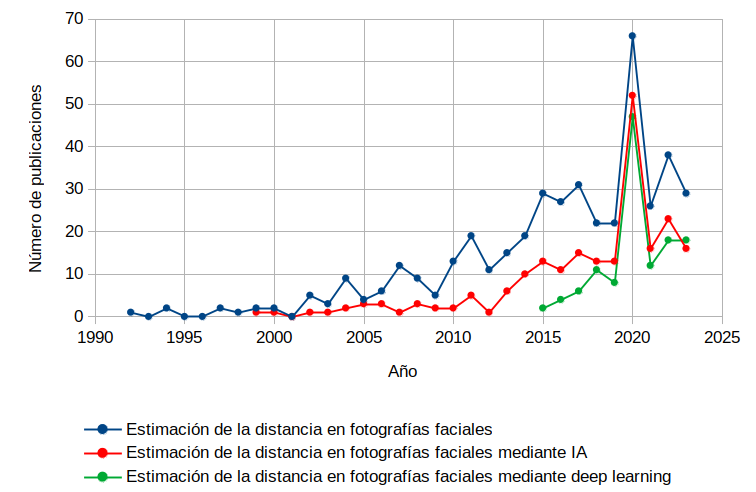
\includegraphics[scale=0.45]{imagenes/cap3/grafica_scopus3.png}
	\caption{Número de publicaciones, en Scopus, relacionadas con la estimación de la distancia en fotografías faciales en función del año de publicación}
	\label{fig5}
\end{figure}

\section{Primeros enfoques}

El primer método utilizado para abordar la estimación métrica del SCD fue propuesto por Flores et al. \cite{28}, se basa en el uso de un conjunto de puntos de referencia de la cara para estimar la posición y la distancia a la cámara en distancias desde 10 cm hasta 3 m. El proceso consiste en, entrenar un modelo de regresión para predecir la distancia entre la cámara y la cara, utilizando un conjunto de imágenes 3D de caras humanas con sus respectivos puntos de referencia faciales (se observa que estas referencias no varían drásticamente entre individuos, sino que se agrupan en 'clusters'). Dicho conjunto de datos 3D solo contiene vistas de frontales y de perfil 3/4. 

Dada una imagen 2D de una cara desconocida, se identifican los puntos de referencia faciales y mediante el algoritmo EPnP \cite{29}, junto con la suposición de que las referencias no varían mucho entre individuos, se infiere la posición 3D de la cara y se utiliza el modelo de regresión previamente entrenado para predecir el valor de la distancia a la cámara.

Algunas de las limitaciones asociados a este primer método son: el uso de un conjunto de datos 3D (no siempre tendremos disponibles imágenes 3D para el entrenamiento), la combinación de diferentes longitudes focales en el mismo dataset o el reconocimiento manual de los puntos de referencia faciales

Posteriormente, en Burgos-Artizzu et al. \cite{30} se propuso un método que no necesitaba la reconstrucción 3D ni la anotación manual de los puntos de referencia de la imagen. Este método utiliza un conjunto de datos llamado Caltech Multi-Distance Portraits (CMDP), compuesto de 53 retratos individuales desde 7 distancias distintas entre 60 cm y 480 cm, para entrenar el modelo. Todas las imágenes del conjunto de datos fueron anotadas manualmente con 55 marcas faciales. 

El método se basa en dos fases: primero, la identificación automática de los puntos de referencia faciales, y después, la estimación de la distancia mediante regresión.

Este nuevo enfoque, a pesar de mejorar lo que previamente se había hecho, sigue teniendo algunas limitaciones como el recorte de las imágenes (pérdida de resolución) o la única vista frontal.

Existen otros métodos que estiman el SCD a partir de características anatómicas como el tamaño de la cara \cite{32}, la distancia de los ojos \cite{33} o una combinación de ambos \cite{34}.

\section{MediaPipe Iris}

MediaPipe Iris \footnote{https://blog.research.google/2020/08/mediapipe-iris-real-time-iris-tracking.html} es un modelo de aprendizaje automático, creado por investigadores de Google, capaz de seguir puntos de referencia (iris, pupila y contornos del ojo) usando una cámara RGB, en tiempo real, y sin necesidad de ningún hardware especializado. A través de los puntos de referencia del iris, el model es capaz de determinar la distancia métrica entre el sujeto y la cámara.

El modelo se basa en el diámetro horizontal del iris del ojo humano, que se mantiene relativamente constante en un rango de 11.7±0.5 mm en una amplia población, esto junto con algunos simples argumentos geométricos, permiten la posibilidad de estimar el SCD.

Este modelo requiere de unas condiciones, que además, son sus principales limitaciones. El modelo solo puede ser usado cuando: existen datos EXIF disponibles; son imágenes frontales donde el iris es visible; y los individuos están a menos de 2m de la posición de la cámara.



\section{PerspectiveX}

PerspectiveX fue el método propuesto por Stephan et al. \cite{21} para la estimación del SCD en fotografías faciales con el fin de mejorar el proceso de superposición craneofacial.

Este método se basa en la localización de una característica anatómica, la longitud de la fisura palpebral entre dos marcas precisas y fácilmente determinables. Se utiliza este rasgo anatómico debido a que: es fácilmente visible en vista frontal e incluso en el lado más cercano a la cámara si la cabeza está girada; está definida por dos puntos de referencia muy precisos; tiene una variación muy ajustada, debido a restricciones evolutivas; es una característica facial relativamente grande, por lo que, minimiza el impacto de los errores en comparación con otras características faciales invariantes como el diámetro del iris; tiene una distribución normal que reduce el error de predicción a la mitad.

Además de la fisura palpebral, PerspectiveX necesita conocer el tipo de cámara y la longitud focal de las lentes, que se pueden extraer siempre de imágenes electrónicas usando lectores EXIF disponibles en internet. El tipo de cámara es necesario para obtener las especificaciones de píxeles.

Finalmente, la estimación del SCD se realiza mediante la siguiente fórmula:

\begin{equation}
	SCD = f (1+\frac{A}{x \cdot y})
\end{equation}

donde: $f$, es la longitud focal de las lentes (mm); $A$, es la longitud real de la fisura palpebral (mm); $x$, es la longitud de la fisura palpebral en la foto (píxeles); $y$, son las especificaciones del tamaño del píxel del receptor de imagen (mm)

Al no disponer de la longitud real de la fisura palpebral, se utiliza el valor medio de un conjunto de individuos agrupados por sexo y edad, ya que, sabemos que la longitud varía muy poco debido a restricciones evolutivas.

Este método permite una precisa estimación del SCD para una longitud focal conocida. Sin embargo, posee algunas limitaciones como: el requerimiento de interacción manual para anotar los puntos de referencia faciales; y que no tiene en cuenta las rotaciones de cabeza de más de 30º.

\section{FacialSCDnet}

FacialSCDnet fue un método propuesto por Bermejo et al. \cite{14}, en el que se estima el SCD, directamente desde las fotografías, mediante la aplicación de técnicas deep learning. El uso de una arquitectura profunda evita una restricción crítica: el requerimiento de detectar una característica anatómica en particular para guiar el proceso de estimación. Es por ello que este método es capaz de estimar el SCD en cualquier posición de la cabeza, desde frontal hasta perfil lateral.

Se utilizó un conjunto de datos de entrenamiento compuesto por dos colecciones: 

\begin{itemize}
	\item Conjunto sintética: se generaron imágenes sintéticas 2D a partir de los modelos 3D de la base de datos Stirling ESRC 3D Face \footnote{Stirling ESRC 3D Face: https://pics.stir.ac.uk/ESRC/index.htm}. En particular, se usaron 315 modelos faciales de 54 indviduos diferentes para generar aproximadamente 150.000 fotografías sintéticas.
	\item Conjunto de fotografías digitales: se adquirieron fotografías de 28 individuos mediante el siguiente protocolo de adquisición: se consideraron 4 longitudes focales diferentes (27 mm, 35 mm, 50 mm, 85 mm) en formato completo; se utilizaron 12 distancias, de la cámara al sujeto, desde 50 cm hasta 6 m; se fotografiaron 7 posiciones diferentes de la cabeza, desde el perfil izquierdo hasta el perfil derecho, a intervalos de 30º de rotación.
\end{itemize}

La función de pérdida utilizada en el modelo, se basa en el error absoluto medio de la distorsión facial relativa:

\begin{equation}
	Distorsion = \frac{\sum_{i=1}^{n} |y_i - x_i|}{n}
\end{equation}

donde $y_i$ son los valores reales (etiquetas) de la distorsión facial, y $x_i$ son los valores predichos de la distorsión facial, calculados a partir del factor de distorsión ($D_f$):

\begin{equation}
	D_f = \frac{1}{1 + \frac{SCD}{d}}
	\label{eq:df}
\end{equation}

En la ecuación \ref{eq:df}, $d = 12.6572 cm$ corresponde a un valor derivado de cálculos geométricos \cite{23} para obtener experimentalmente el factor de distorsión de una cabeza humana de tamaño promedio, según el SCD de la fotografía.

FacialSCDnet está compuesto por 4 modelos de deep learning, cada uno asociado a una longitud focal de las utilizadas en el conjunto de datos. La estructura de cada CNN se basa en una arquitectura VGG-16, cuyos pesos están inicializados a los pre-entrenados con ImageNet \footnote{ImageNet: https://www.image-net.org/}. Para adaptar la arquitectura al problema de estimación del SCD, los 5 bloques convolucionales se mantienen, se elimina la capa superior, y se añaden 2 capas totalmente conectadas que se entrenarán desde cero. Finalmente, la última capa del modelo consistirá en una activación lineal que realiza la tarea de regresión.

El proceso de entrenamiento de los modelos tuvo dos fases. Primero, los modelos fueron entrenados con el conjunto de datos sintético para aprender relaciones entre SCD y características faciales. Después, se utiliza un ajuste fino usando el conjunto de datos real.






\chapter{Materiales y métodos}
\thispagestyle{empty}

\section{Materiales}

En este TFG se generará un conjunto de datos de imágenes sintéticas fotorrealistas a partir de varios modelos 3D seleccionados.

\subsection{Modelos 3D}

Se llevó a cabo un análisis exhaustivo de las bases de datos disponibles de modelos 3D de personas. Tras la búsqueda, se utilizaron diversos conjuntos de datos públicos con el objetivo de crear un conjunto de datos unificado, realista y diverso. En este conjunto, se incluyeron tanto modelos faciales como modelos de cuerpo completo, todos ellos con sus correspondientes texturas.

\subsubsection{Modelos faciales}
Se han seleccionado los siguientes conjuntos de datos: HeadSpace \cite{60}, H3DS-net \cite{61} y DI4D\_UGR\_ANON \footnote{Conjunto de datos proporcionado por el tutor}.

El conjunto de datos de Headspace \cite{60} es un conjunto de imágenes en 3D de la cabeza humana, que consta de 1519 sujetos que llevan gorros de látex ajustados para reducir el efecto de los peinados. Las ventajas de este conjunto son que tienen muy buena resolución y además incluye metadatos útiles para seleccionar un subconjunto de datos adecuado.

\begin{figure}[h]
	\centering
	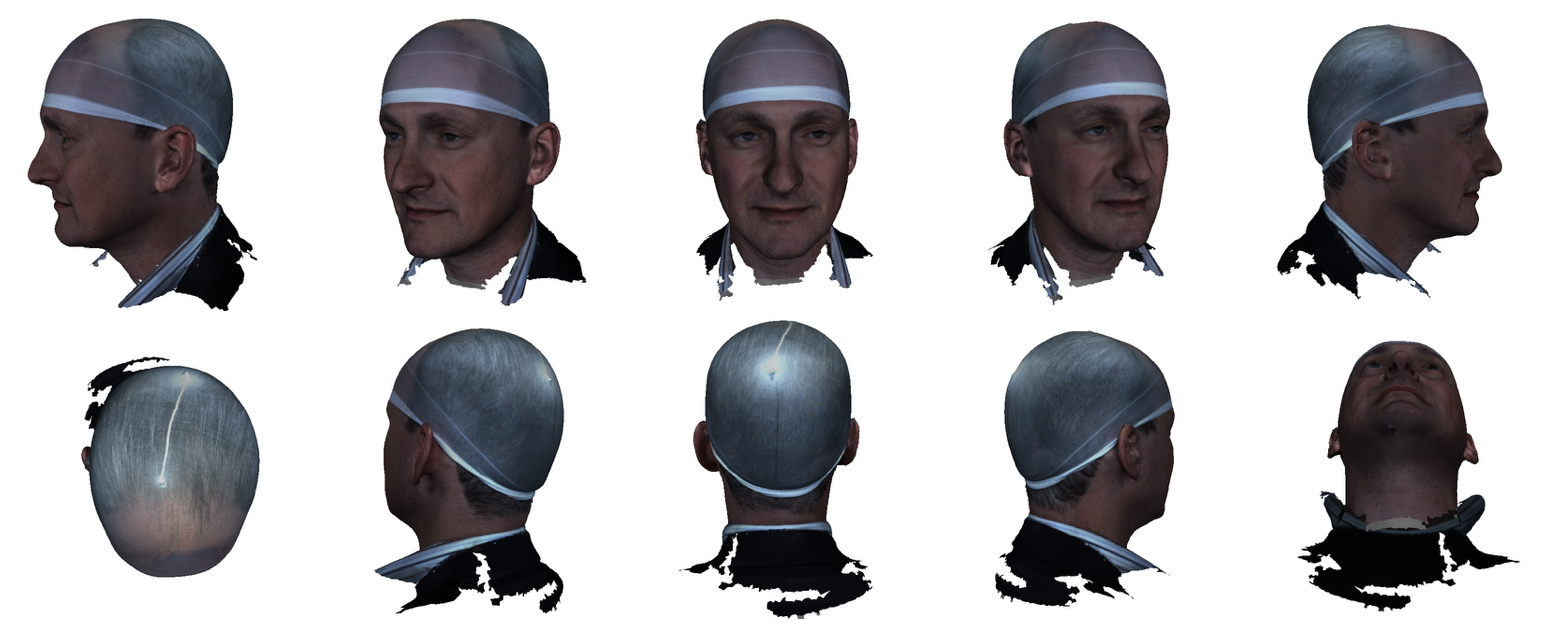
\includegraphics[scale=0.075]{imagenes/cap4/headspace.png}
	\caption[Ejemplos HeadSpace 3D.]{Ejemplos de modelos en HeadSpace 3D.}
	\label{fig17}
\end{figure}

H3DS-net \cite{61} contiene escaneos texturizados en 3D de la cabeza completa con una alta resolución. Este conjunto comprende un total de 23 modelos, todos ellos con los ojos cerrados, lo que añade una variabilidad adicional.

\begin{figure}[h]
	\centering
	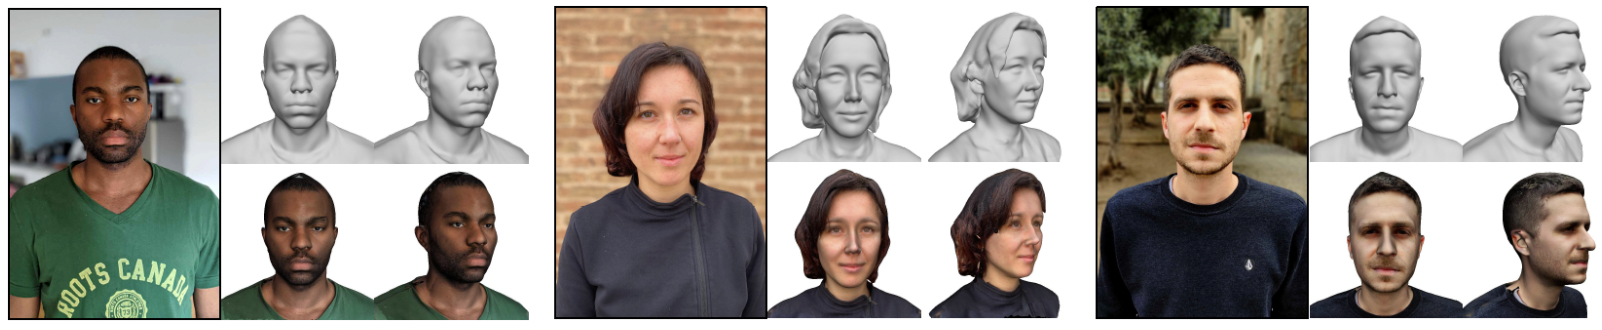
\includegraphics[scale=0.18]{imagenes/cap4/h3dsnet.png}
	\caption[Ejemplos H3DS-net.]{Ejemplos de modelos en H3DS-net.}
	\label{fig18}
\end{figure}

DI4D\_UGR\_ANON es un conjunto de datos creado por la Universidad de Granada...

Si bien se investigaron otros conjuntos de datos como FaceVerse \cite{64} o CASIA \footnote{http://biometrics.idealtest.org/}, estos fueron descartados debido a problemas como la baja calidad, formatos incompatibles y escalas no reales.

\subsubsection{Modelos de cuerpo entero}
Se han seleccionado los siguientes conjuntos de datos: HuMMan \cite{62}, People Snapshot \cite{63} y Render People \footnote{https://renderpeople.com/es/}

HuMMan \cite{62} es un conjunto de datos 3D que consta de 153 sujetos humanos, con una amplia cobertura de sexos biológicos, edades, formas del cuerpo y poblaciones. Cada sujeto contiene 2-3 secuencias, y cada secuencia contiene aproximadamente 20 modelos.

\begin{figure}[h]
	\centering
	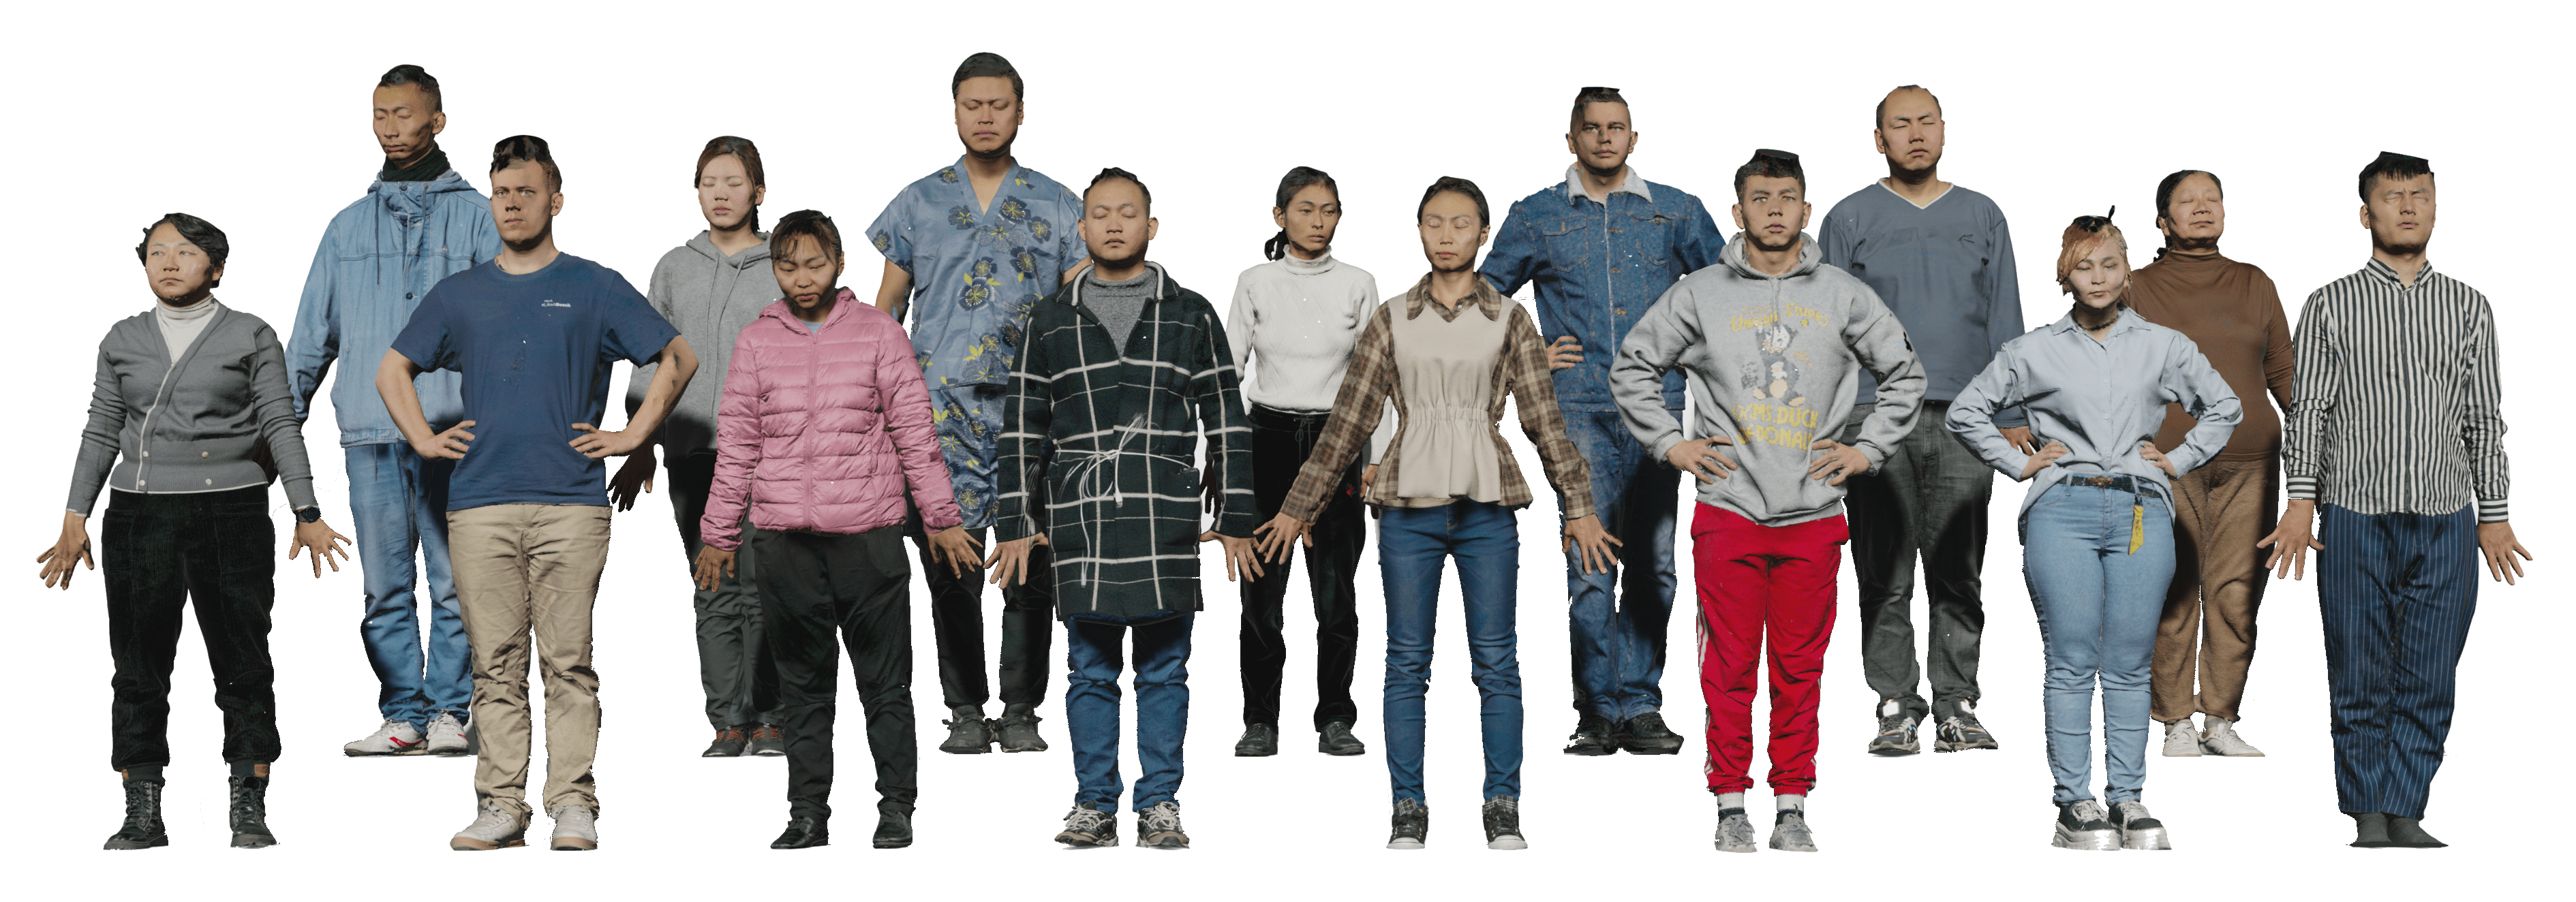
\includegraphics[scale=0.4]{imagenes/cap4/humman.png}
	\caption[Ejemplos HuMMan.]{Ejemplos de modelos en HuMMan.}
	\label{fig19}
\end{figure}

People Snapshot \cite{63} contiene 24 sujetos 3D en diferentes situaciones tales como casual, deporte y actividades al aire libre.

\begin{figure}[h]
	\centering
	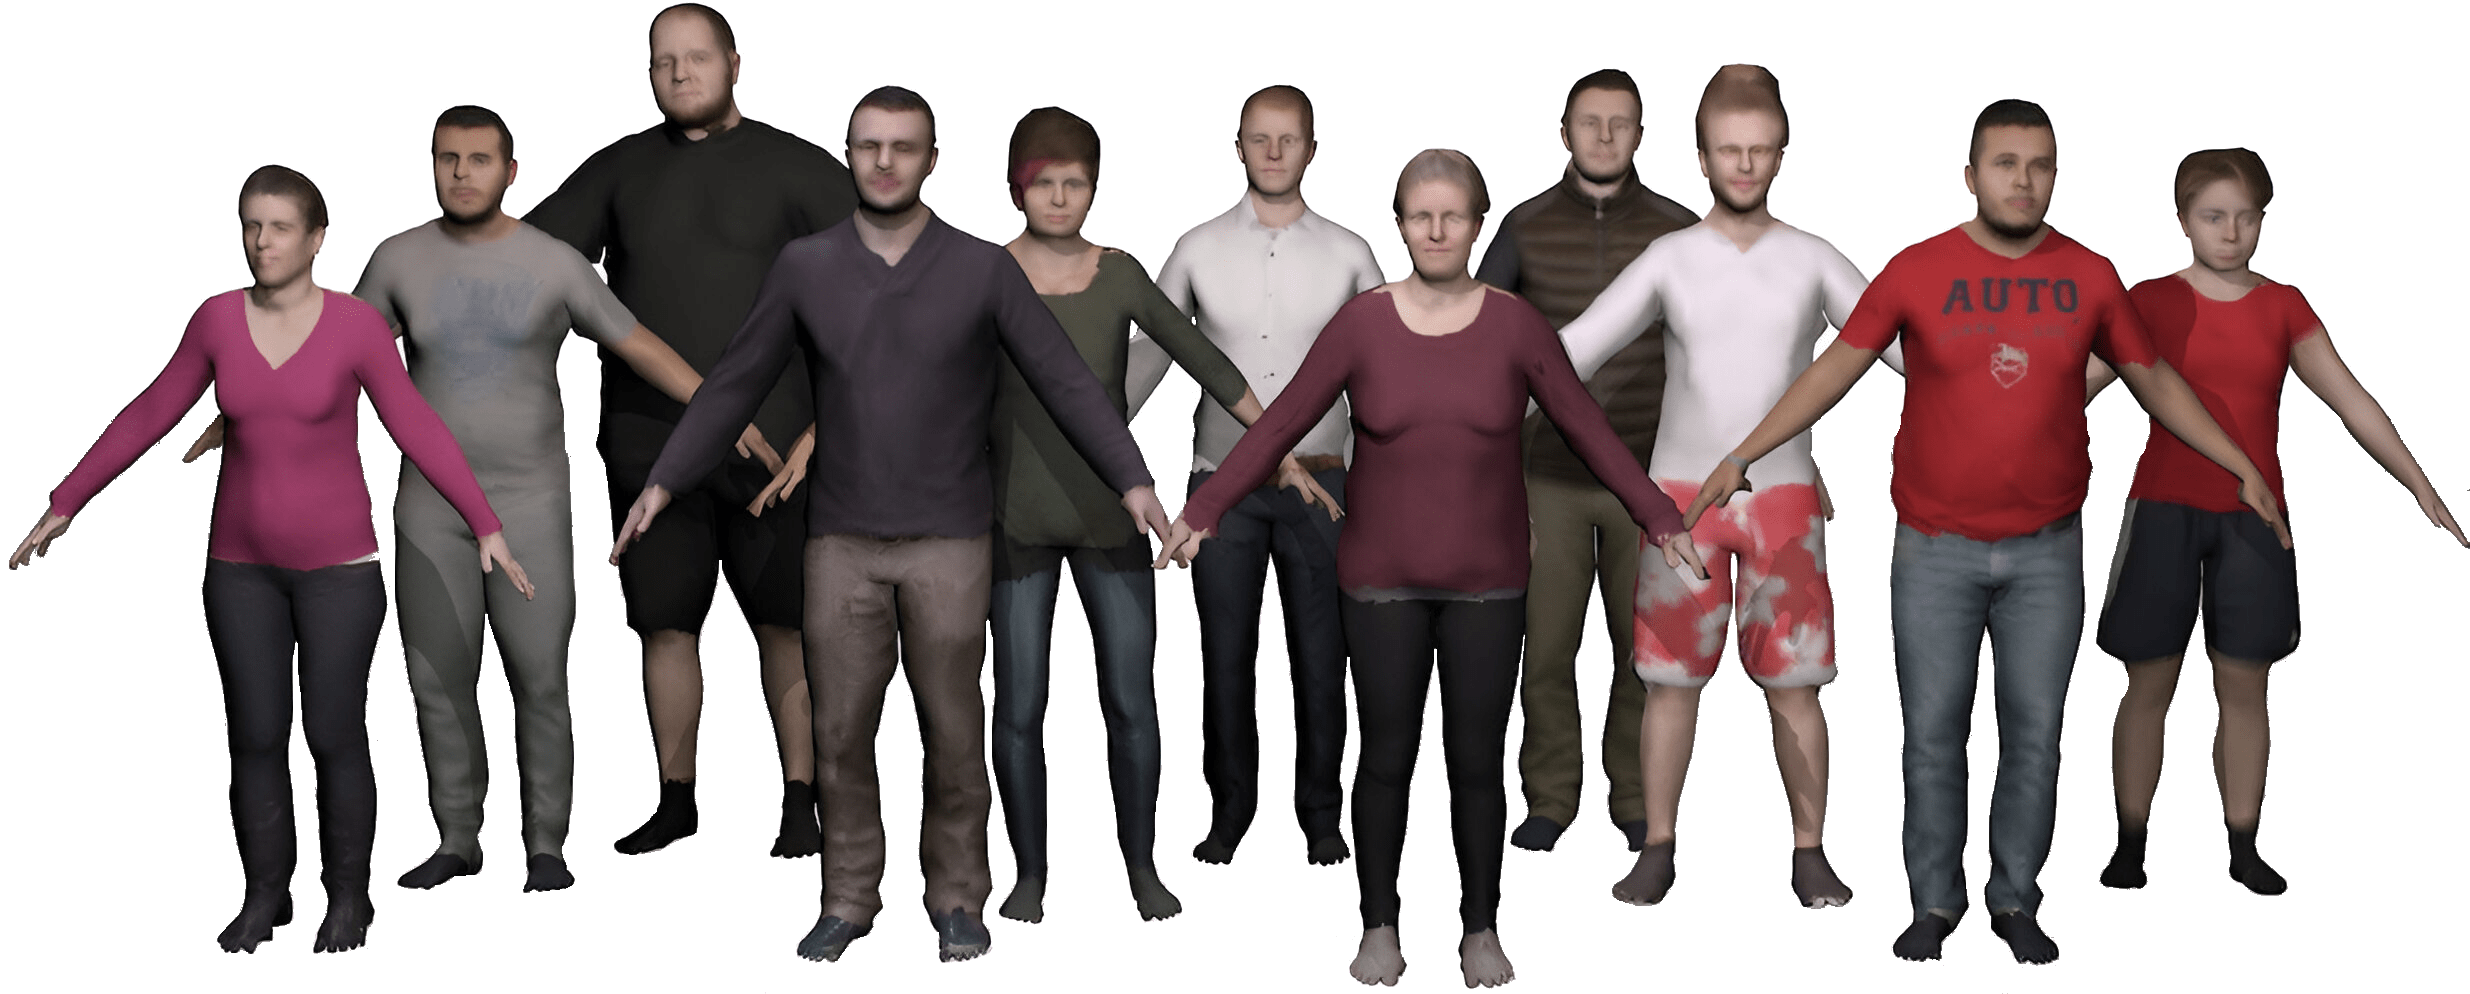
\includegraphics[scale=0.5]{imagenes/cap4/snapshot.png}
	\caption[Ejemplos People Snapshot]{Ejemplos de modelos en People Snapshot.}
	\label{fig20}
\end{figure}

RenderPeople es una empresa privada especializada en la creación de modelos humanos en 3D. Existen modelos disponibles para comprar, pero dado su costo, hemos decidido emplear exclusivamente aquellos gratuitos que están disponibles. Aunque únicamente hay 2, estos son bastante realistas y presentan situaciones que no se contemplan en los anteriores modelos.

\begin{figure}[h]
	\centering
	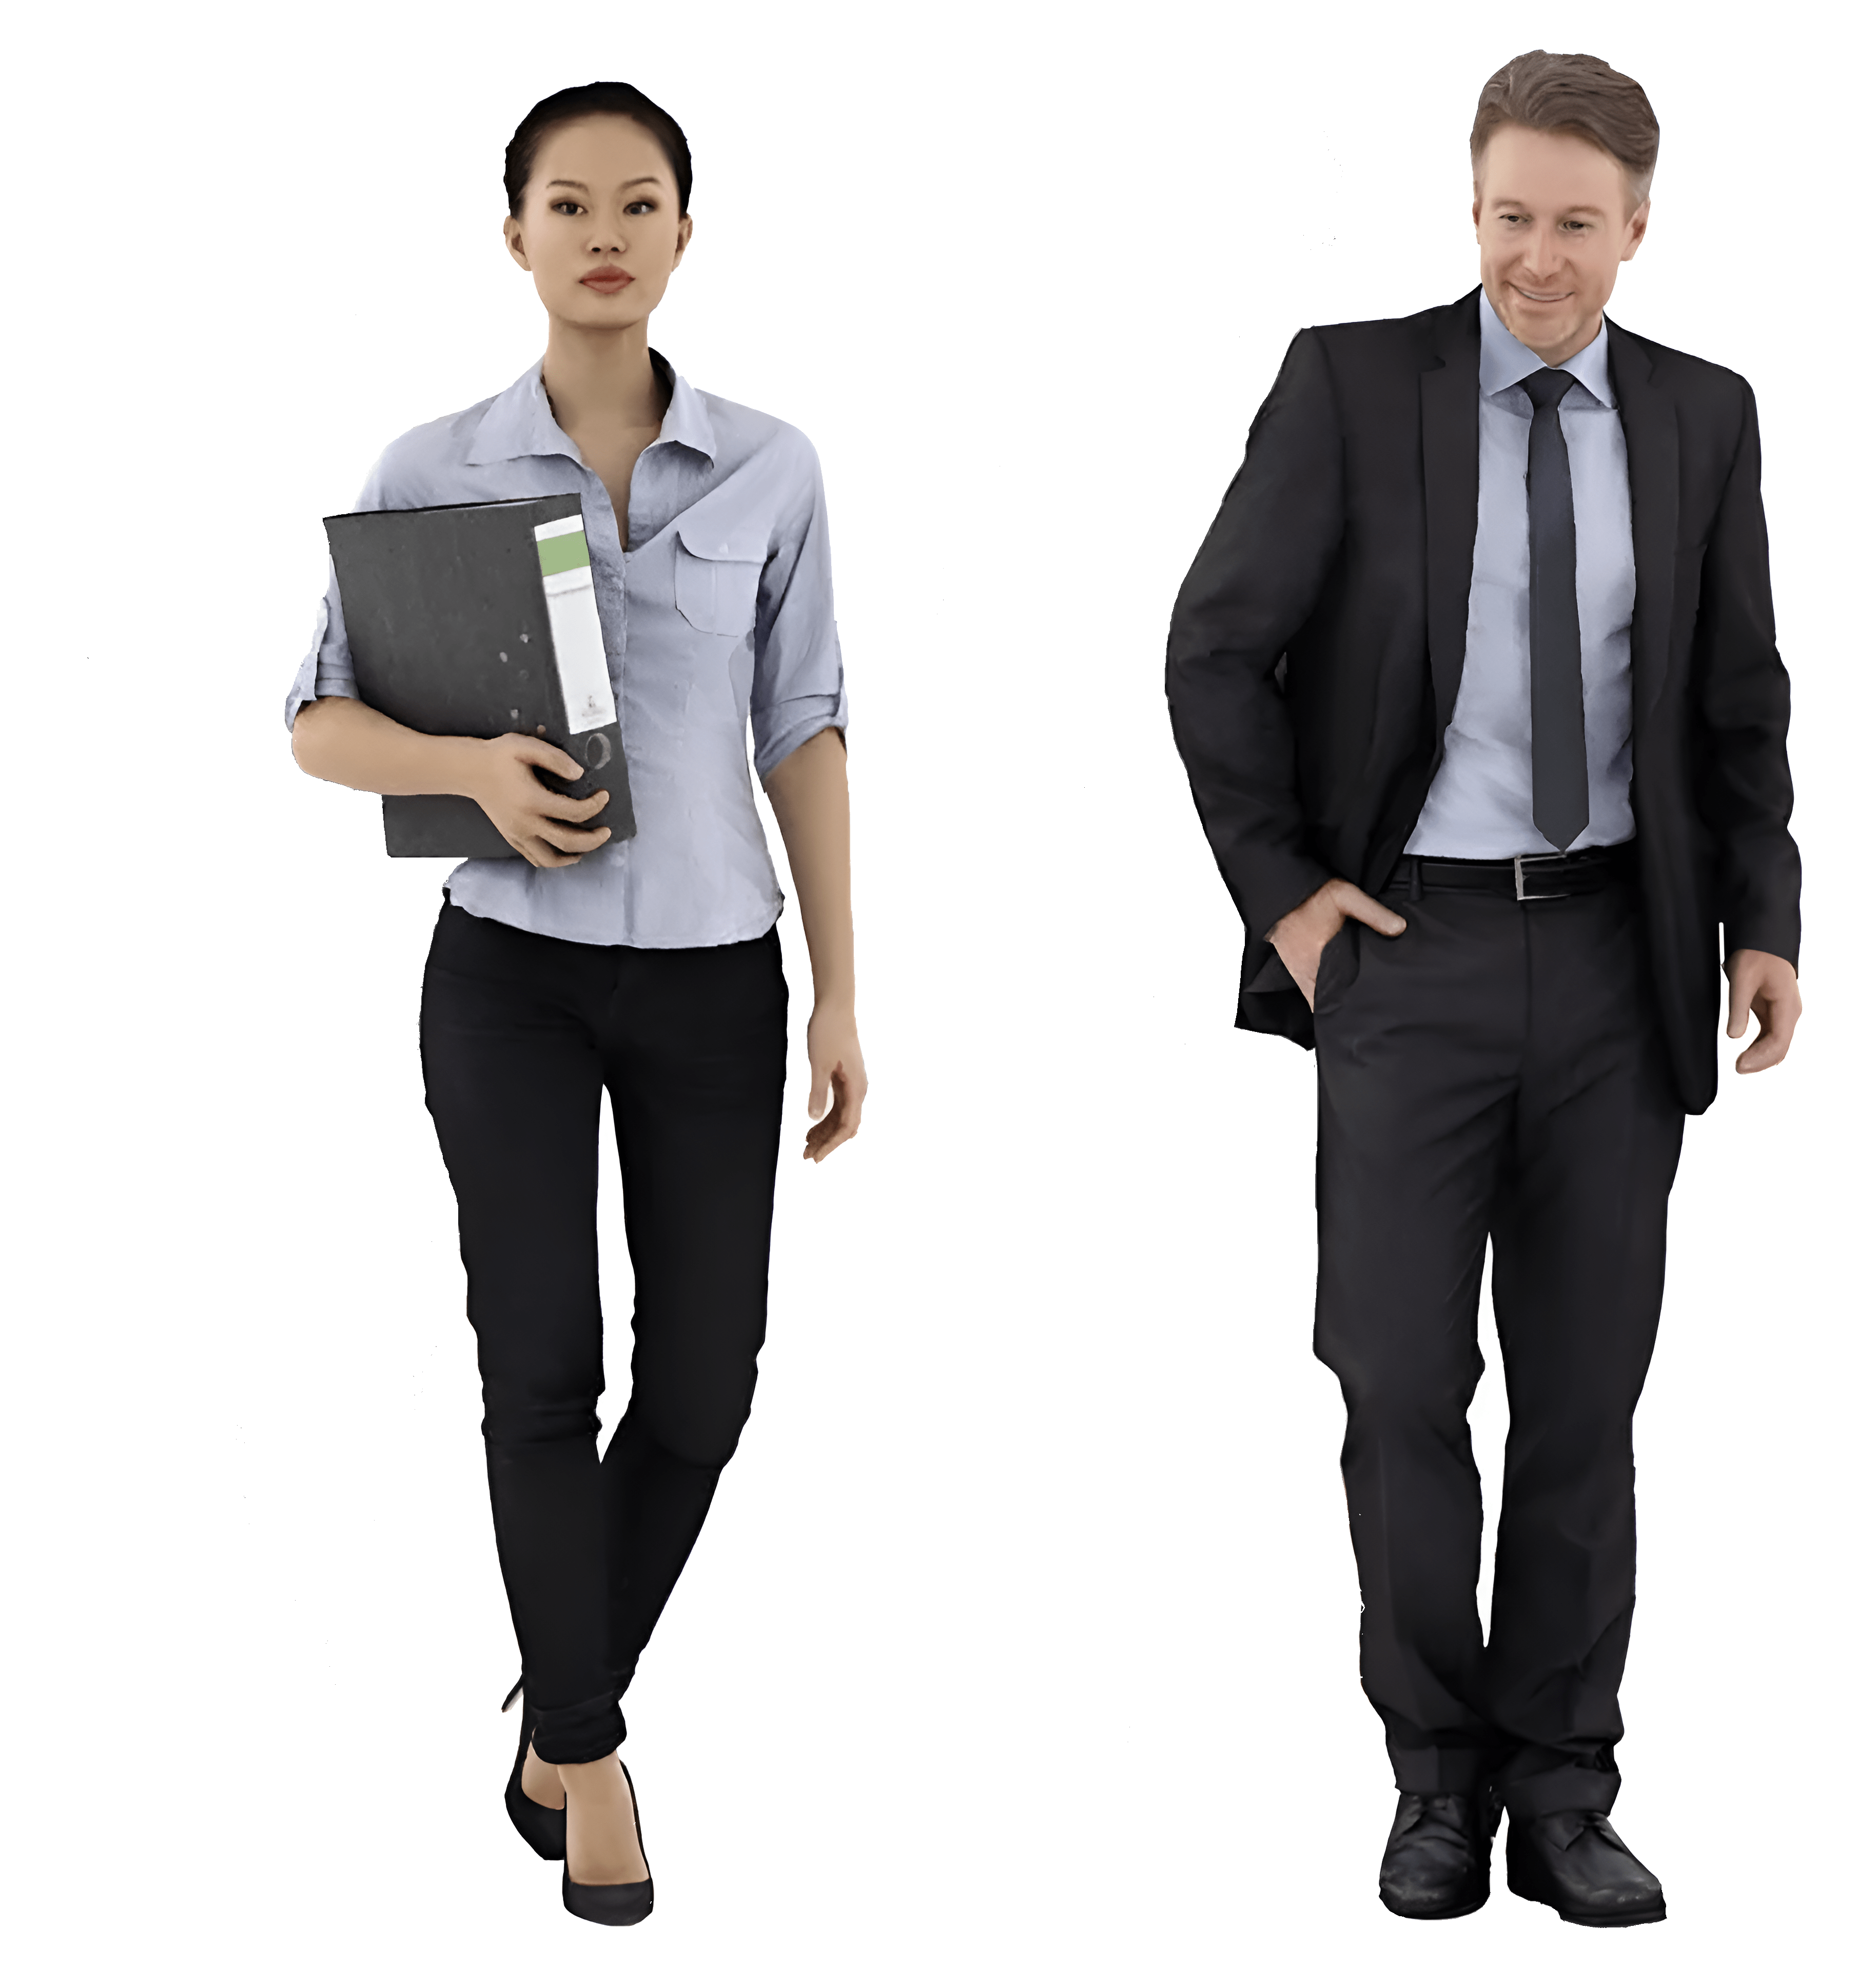
\includegraphics[scale=0.04]{imagenes/cap4/renderpeople.png}
	\caption[Ejemplos Render People]{Ejemplos de modelos en Render People.}
	\label{fig21}
\end{figure}

\subsubsection{Selección del subconjunto de modelos}

Ante la gran cantidad de modelos disponibles, surge la necesidad de elegir un subconjunto de modelos adecuado, combinando modelos faciales y de cuerpo completo.
En total, se han seleccionado 176 modelos 3D, de los cuales 106 son modelos faciales y 70 son modelos de cuerpo completo.

En primer lugar, de H3DS-net se han seleccionado los 23 modelos, compuestos por 13 masculinos y 10 femeninos, todos ellos de ascendencia europea. 
De HeadSpace, se han elegido 73 modelos, de los cuales 36 son masculinos y 37 femeninos. Esta selección incluye modelos de ascendencia europea, asiática, africana o combinada. Además, todos los modelos son mayores de 14 años.
Respecto a DI4D\_UGR\_ANON, se han seleccionado 10 modelos, compuestos por 6 femeninos y 4 masculinos, todos ellos de ascendencia europea.

Además, se han seleccionado los 2 modelos provenientes de RenderPeople, uno masculino y otro femenino, ambos de ascendencia europea.
De People Snapshot se han seleccionado los 24 modelos, de los cuales 16 son masculinos y 8 femeninos, todos de ascendencia europea.
Finalmente, se han seleccionado 44 modelos de HuMMan, distribuidos en 23 modelos masculinos y 21 modelos femeninos. En este conjunto, 28 modelos son de ascendencia asiática, 11 son de ascendencia africana y 5 son de ascendencia europea.

Estas selecciones se realizaron con el objetivo de incluir la mayor diversidad posible en términos de sexos biológicos y ascendencias, teniendo en cuenta las bases de datos disponibles.

\subsection{Preparación del conjunto de datos}

\subsubsection{Procesamiento de modelos 3D}

Al contar con un conjunto de datos compuesto por múltiples conjuntos, cada uno con una escala específica, ya sea en centímetros o metros, y dispuestos de manera diversa, surge la necesidad de normalizar la escala y alinear los modelos con respecto a un punto de referencia. Para esto, se emplearán los ojos como punto de origen (0, 0, 0), dado que son fácilmente visualizables, se ubican en una posición central y están presentes tanto en los modelos faciales como en los de cuerpo completo. Este procesamiento se produce para luego poder generar correctamente las imágenes a distintas distancias.

La normalización de la escala se lleva a cabo mediante transformaciones de escala, multiplicando o dividiendo por un factor de 100. Esta se realiza solo en algunos modelos, para que todos estén a la misma escala.

Para alinear los modelos, en primer lugar se aplicó un \textit{script} de \textit{Python} para realizar transformaciones (específicas para cada conjunto de datos) con el objetivo de posicionarlos de frente. Posteriormente, se desarrolló un programa en \textit{Python} que utiliza librerías como \textit{VTK}, \textit{PyVista} y \textit{Trimesh} para la manipulación de mallas 3D, junto con \textit{Mediapipe} para la detección de rostros. El proceso implica tener un modelo de referencia ya alineado manualmente, junto con 13 puntos de referencia faciales 3D (incluyendo la nariz, los ojos y la boca) obtenidos mediante \textit{Mediapipe}. Después, dado un nuevo modelo sin alinear, se calculan sus puntos de referencia correspondientes y se determina y aplica la matriz de transformación entre estos puntos y los del modelo de referencia.

A excepción de algunos ajustes manuales en los modelos de HeadSpace y HuMMan, el proceso se automatizó de forma efectiva.

\subsubsection{Generación de imágenes faciales sintéticas}

Una vez procesados los modelos 3D, se procedió a generar el conjunto de imágenes faciales. Para ello, se utilizó un \textit{script} en \textit{Blender} que realiza las siguientes tareas para cada modelo:

\renewcommand{\theenumii}{\arabic{enumii}}

\begin{enumerate}
	\item Carga el modelo y lo posiciona a una distancia específica de la cámara. Se seleccionaron 27 distancias distintas, que van desde 50 cm hasta 6m, con incrementos graduales de 5 cm, 10 cm, 20 cm, 25 cm, 50 cm y 1 m.
	\item Posteriormente, para cada distancia, se ajusta la longitud focal de la cámara. Se utilizaron 4 longitudes focales, incluyendo 27 mm, 35 mm, 53 mm y 83.6 mm.
	\item A continuación, para cada longitud focal, se realizan 14 iteraciones, donde en cada iteración:
	\begin{enumerate}
		\item Se aplica un fondo HDR seleccionado aleatoriamente de un conjunto de 95 fondos HDR descargados de Poly Haven \footnote{https://polyhaven.com}.
		\item Se aplican transformaciones aleatorias de rotación de la cámara con respecto al modelo para añadir variabilidad a las poses. Estas transformaciones incluyen tanto rotaciones horizontales (entre -70º y 70º) para mostrar los modelos desde diferentes perspectivas laterales como se muestra en la Figura \ref{fig22}, así como rotaciones verticales (entre -30º y 30º) para presentar perspectivas más altas o bajas como se muestra en la Figura \ref{fig23}.
		\item Se realizan pequeñas traslaciones de la cámara para evitar que todos los modelos aparezcan centrados en la imagen, añadiendo así una variabilidad extra.
		\item Se ajusta la iluminación y las sombras mediante una lámpara cuya intensidad y posición varían aleatoriamente dentro de unos rango determinados.
		\item Por último, se genera la imagen con un tamaño de 224x224 píxeles.
	\end{enumerate}
\end{enumerate}

\begin{figure}[h]
	\centering
	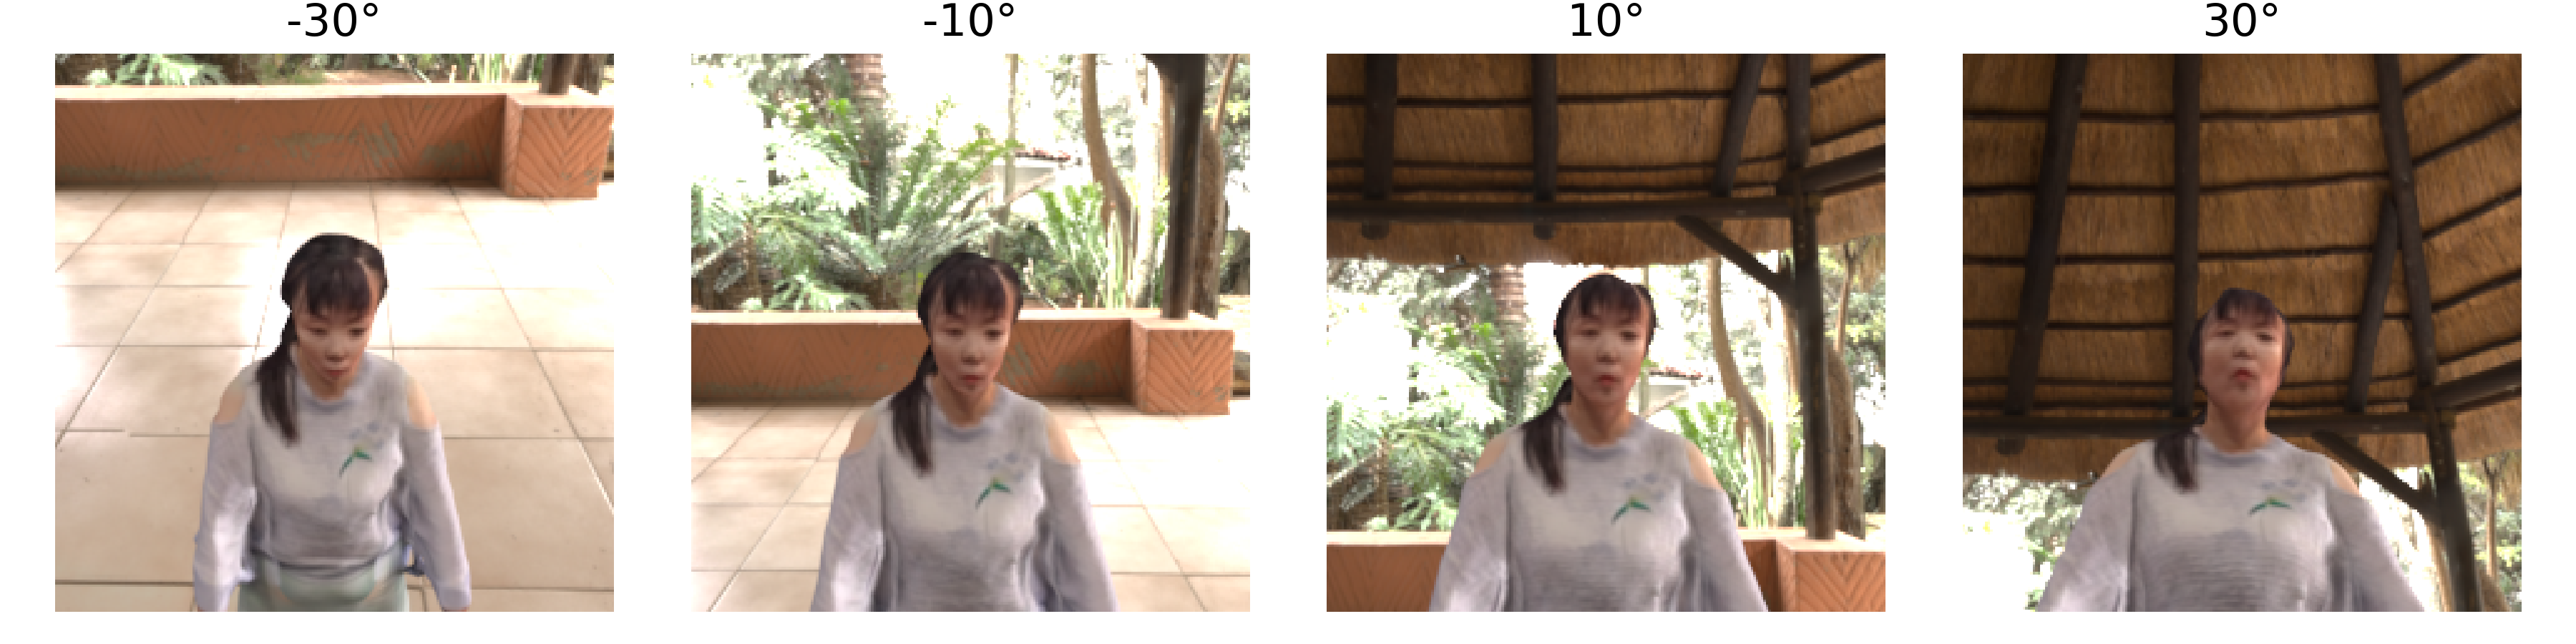
\includegraphics[scale=0.4]{imagenes/cap4/imagenes_rotacion_vertical.png}
	\caption[Ejemplos de imágenes rotadas verticalmente.]{Imágenes generadas desde perspectivas más altas o más bajas.}
	\label{fig22}
\end{figure}

\begin{figure}[h]
	\centering
	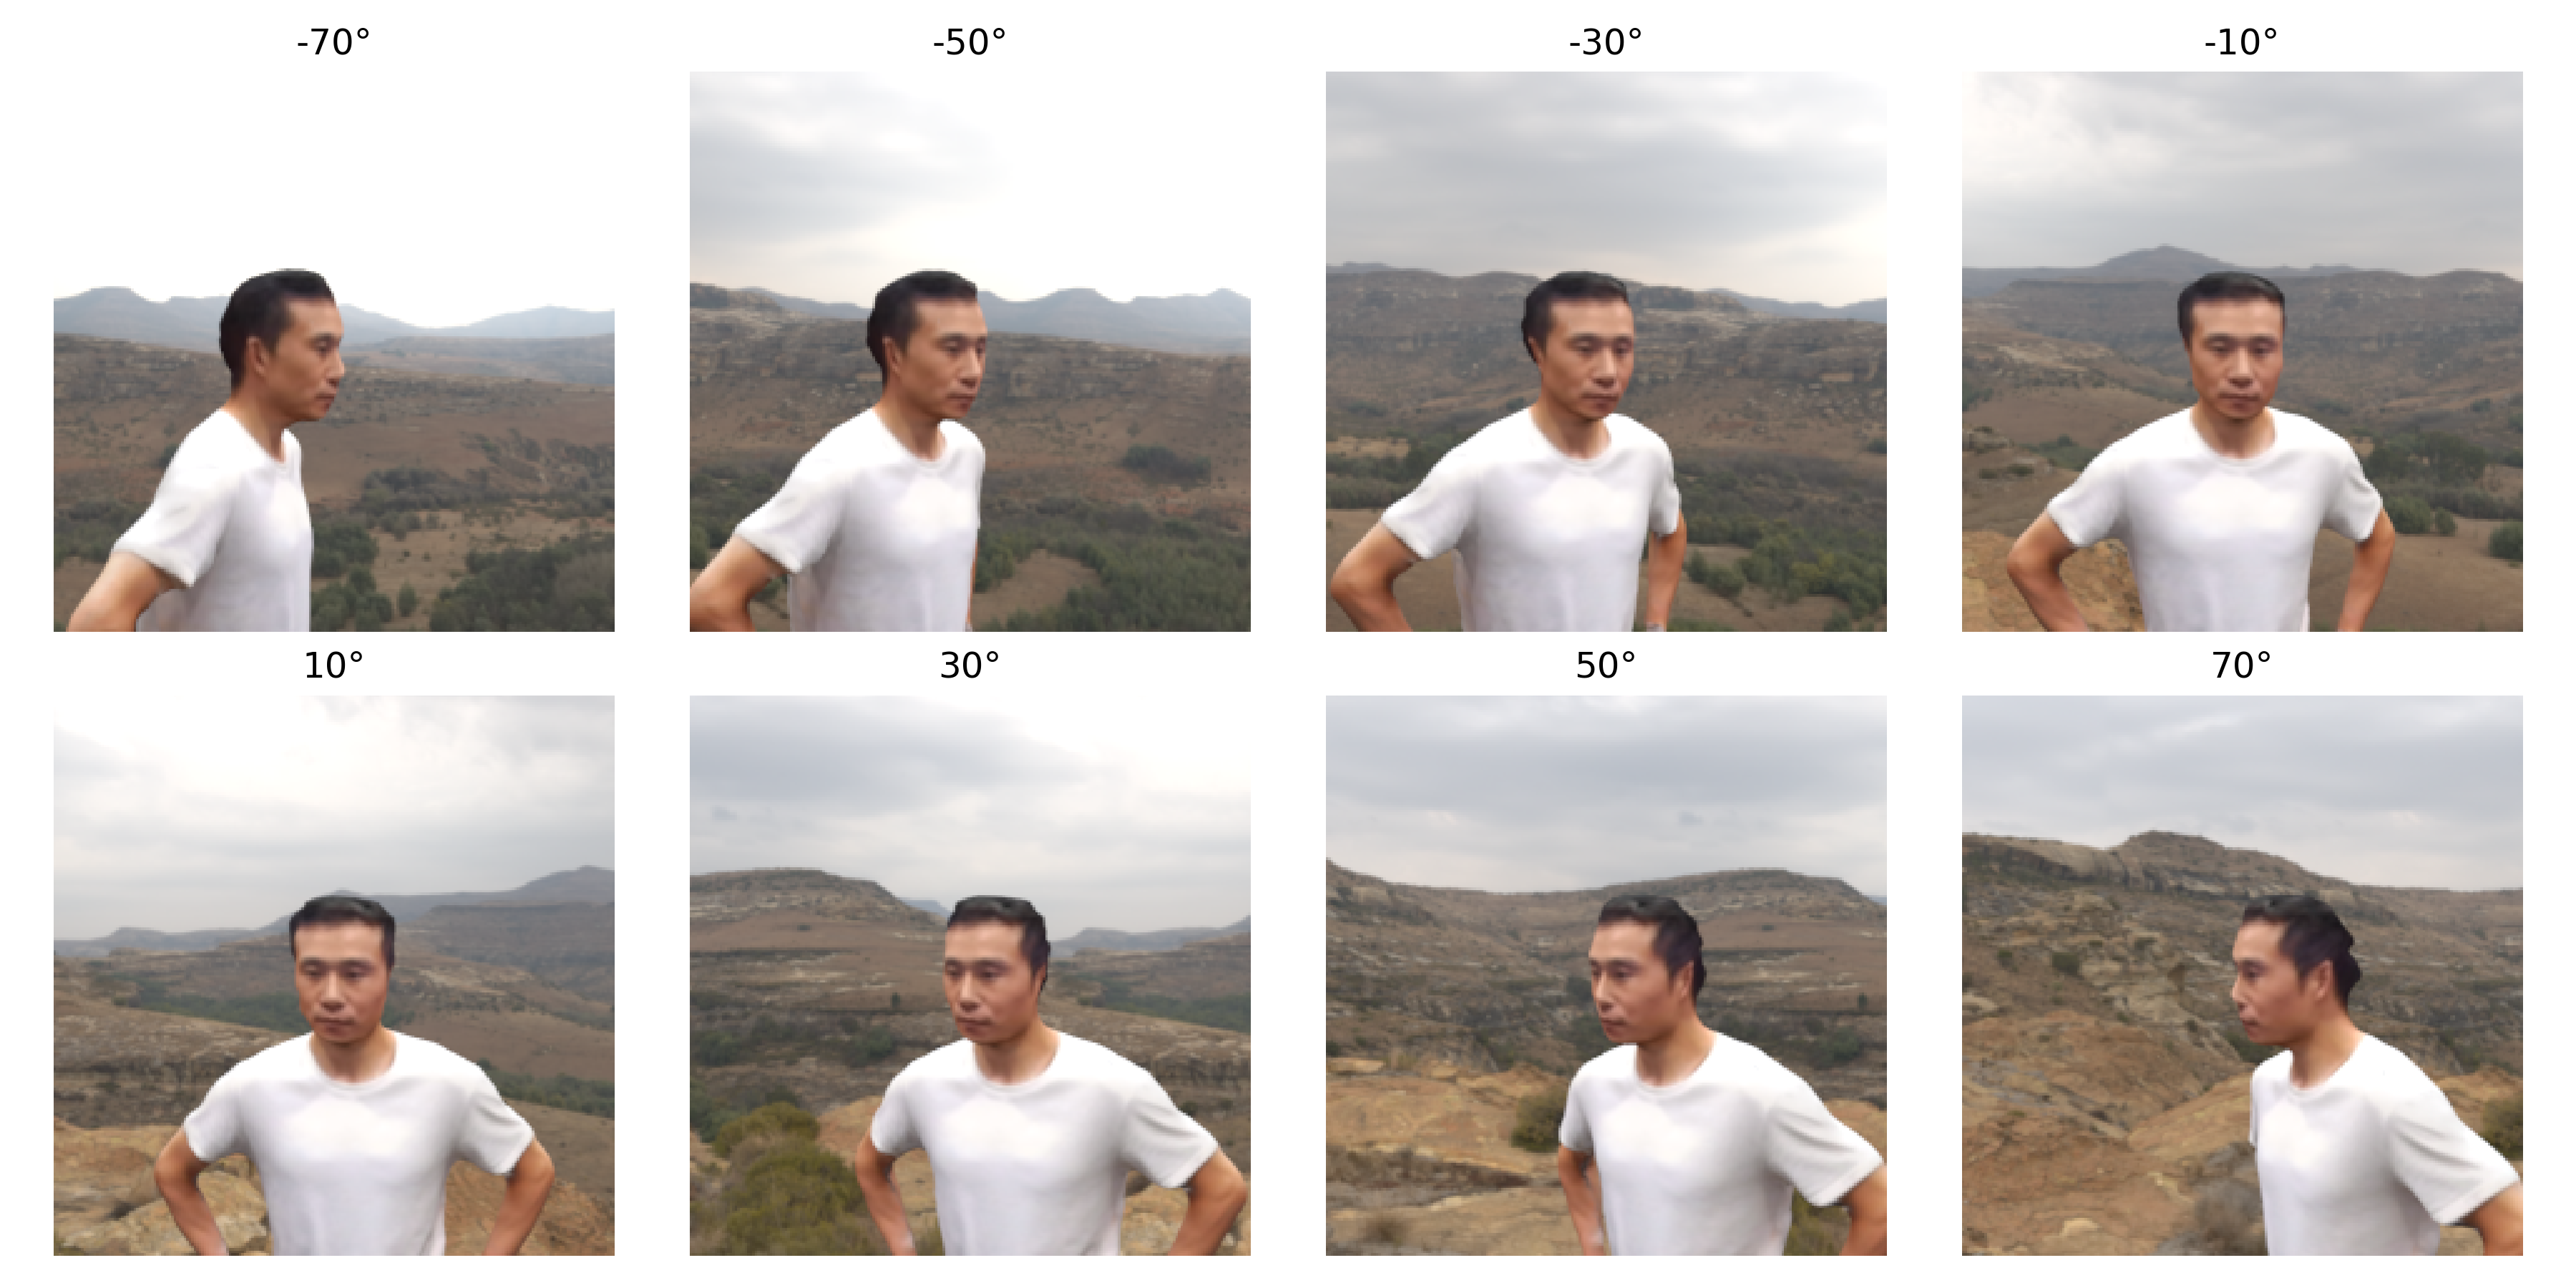
\includegraphics[scale=0.4]{imagenes/cap4/imagenes_rotacion_horizontal.png}
	\caption[Ejemplos de imágenes rotadas horizontalmente.]{Imágenes generadas desde distintas perspectivas laterales.}
	\label{fig23}
\end{figure}

Tras este proceso de generación de imágenes, y considerando que se contaba con 176 modelos 3D, el conjunto total de datos ascendió a 266112 imágenes, es decir, 66528 imágenes por cada longitud focal. Se pueden ver algunos ejemplos de imágenes en la Figura \ref{fig24}.

\begin{figure}[h]
	\centering
	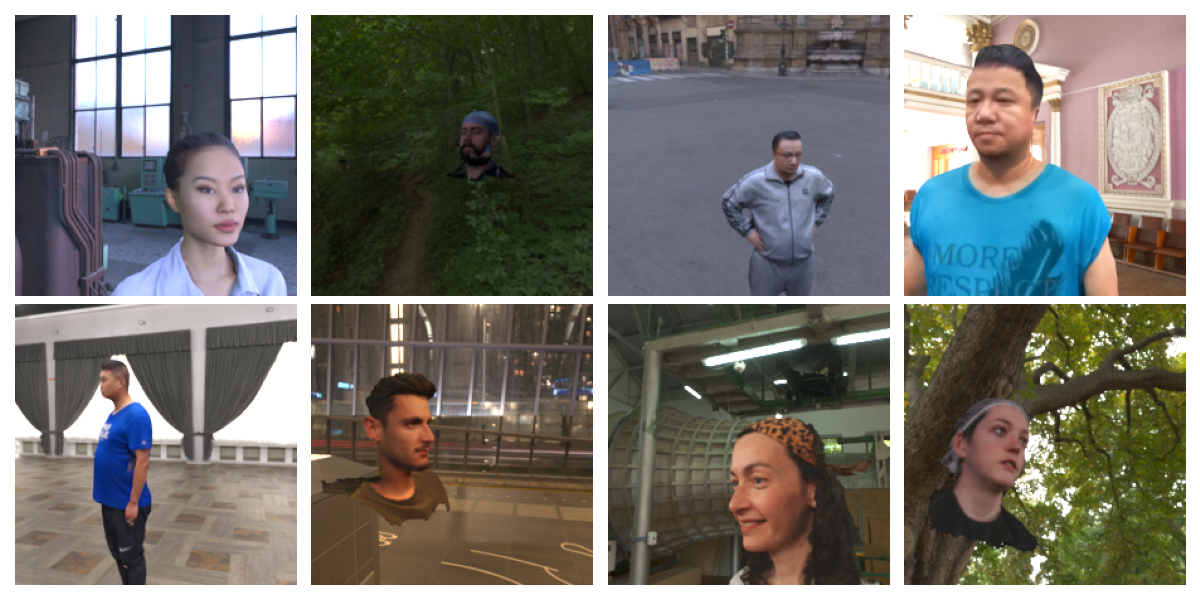
\includegraphics[scale=0.45]{imagenes/cap4/ejemplos_dataset.png}
	\caption[Ejemplos de imágenes generadas para el conjunto de datos.]{Imágenes generadas para el conjunto de datos sintético. Estos ejemplos contienen diferentes sujetos, longitudes focales y distancias.}
	\label{fig24}
\end{figure}

La mejora con respecto al conjunto de datos utilizado en FacialSCDnet \cite{14} es evidente, como se observa claramente en la figura \ref{fig24.1}.

\begin{figure}[h]
	\centering
	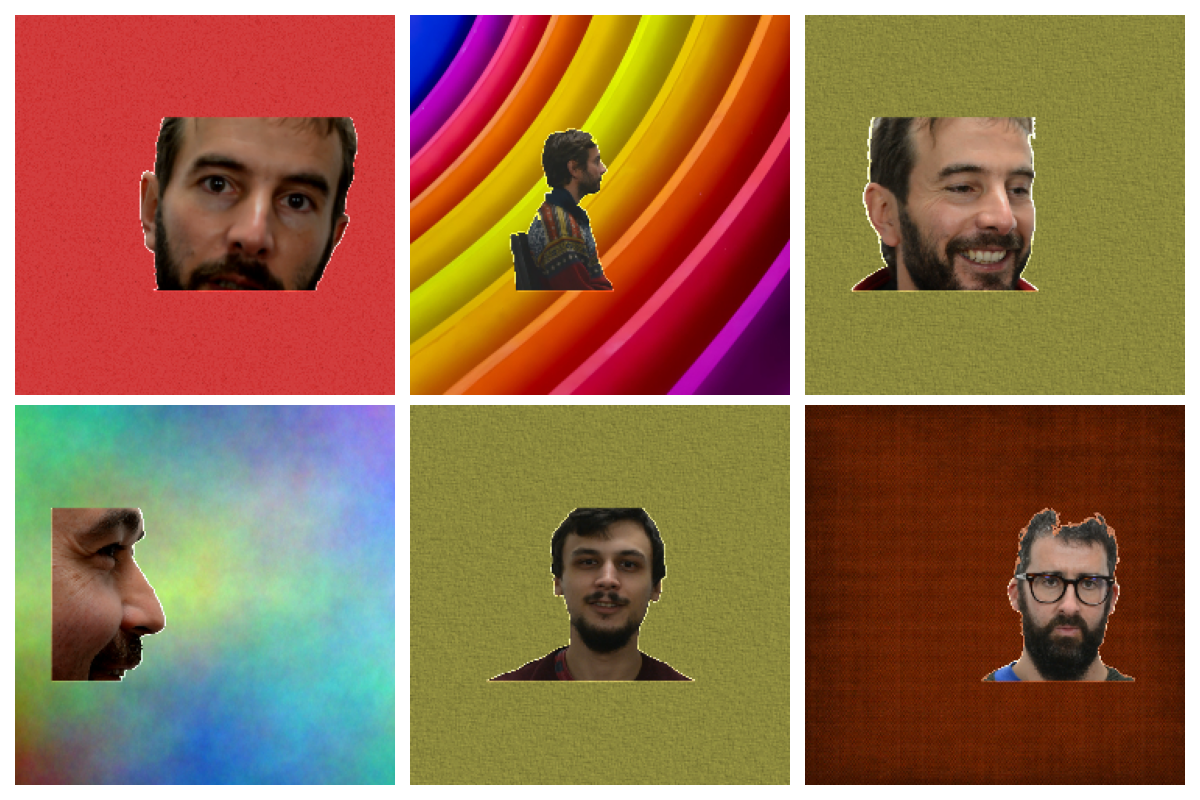
\includegraphics[scale=0.3]{imagenes/cap4/figura_FSCDnet.png}
	\caption[Ejemplos de imágenes utilizadas en FacialSCDnet.]{Imágenes utilizadas en FacialSCDnet \cite{14}.}
	\label{fig24.1}
\end{figure}

\section{Métodos}

En este apartado se describen las arquitecturas \textit{deep learning} que se van a utilizar para realizar los experimentos.

\subsection{FacialSCDnet+}

El método FacialSCDnet+, basado en FacialSCDnet \cite{14}, es un enfoque de aprendizaje profundo para estimar la distancia entre el sujeto y la cámara en fotografías faciales. Se basa en una red neuronal convolucional (CNN) diseñada para regresar la distancia métrica de los individuos directamente desde las fotografías faciales. Este método tiene cuatro modelos de aprendizaje, uno por cada longitud focal presente en el conjunto de datos.
A diferencia de FacialSCDnet, este método utiliza un conjunto de datos totalmente sintético, el cual es mucho más realista y diverso. Además, se ha rediseñado el sistema de aumento de imágenes aplicando las operaciones siguientes:

\begin{itemize}
	\item Transformaciones afines: Se aplican rotaciones aleatorias de hasta 15 grados en sentido horario o antihorario, así como traslaciones horizontales y verticales de hasta el 20\% del tamaño de la imagen, con una probabilidad del 100\%. Esta transformación simula diferentes perspectivas de las imágenes.
	\item Emborronado Gaussiano: Se aplica un emborronado gaussiano con un \textit{kernel} de tamaño 5 y un sigma aleatorio entre 0.1 y 2.0, lo que suaviza la imagen, con una probabilidad del 25\%. Esta transformación ayuda a introducir algo de ruido en las imágenes.
	\item Nitidez: Se ajusta la nitidez de la imagen aplicandole un factor de nitidez de valor 2, con una probabilidad del 25\%. Esta transformación simula una mejor definición de las imágenes
	\item Alteraciones de color: Se aplican ajustes aleatorios en el brillo, contraste y tono de la imagen, con un rango de variación entre $\pm$ 0.1 en cada canal, con una probabilidad del 25\%. Esta transformación contribuye a aumentar la diversidad en la apariencia de las imágenes.
	\item Borrado de píxeles: Se borran zonas de píxeles aleatorias de la image. Estas zonas tienen un tamaño de entre el 2\% y el 5\% de la imagen, y la relación de aspecto está entre un 0.5 y un 1.5, dotando a estas zonas de un aspecto más rectangular. Esta transformación tiene una probabilidad del 25\%. Esta transformación introduce un grado adicional de variabilidad y robustez frente a la ocultación parcial de información.
	\item Escala de grises: La imagen se convierte a escala de grises, perdiendo la información de color, con una probabilidad del 25\%. Esta transformación permite al modelo mejorar su invarianza al color.
\end{itemize}

\begin{figure}[h]
	\centering
	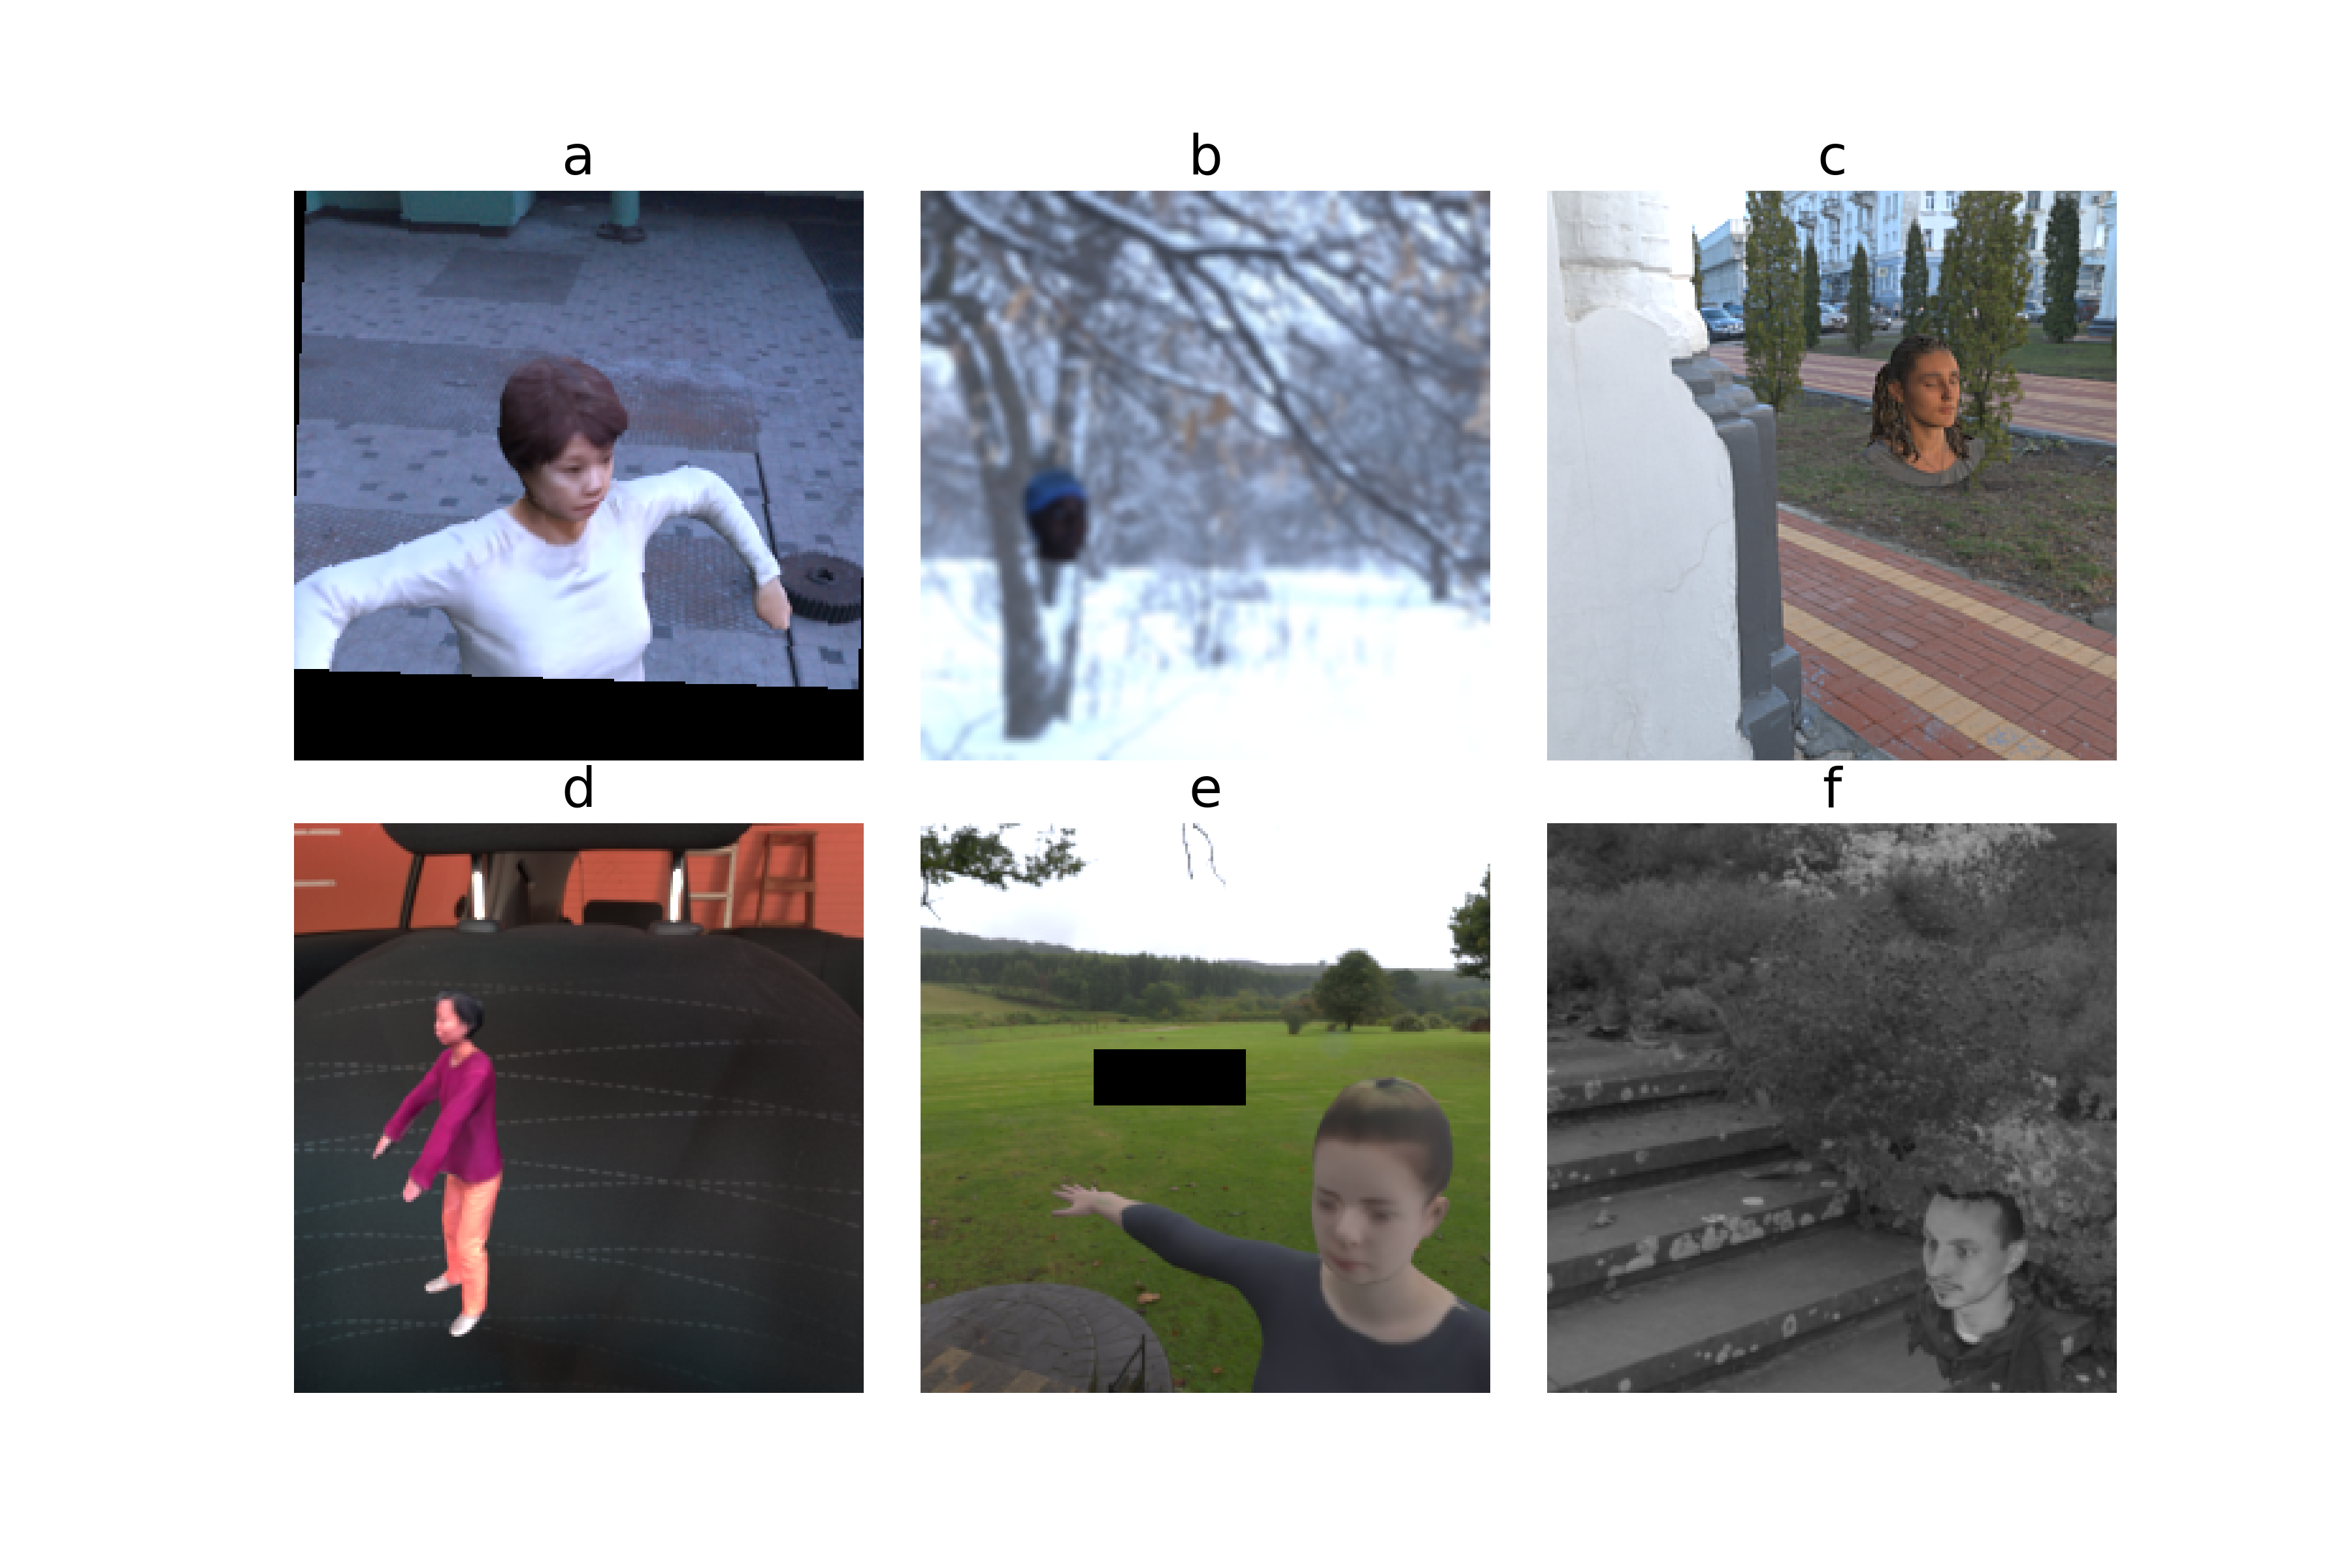
\includegraphics[scale=0.4]{imagenes/cap4/augmented_images.png}
	\caption[Transformaciones utilizadas en el aumento de datos.]{Transformaciones aplicadas a las imágenes: a) transformaciones afines, b) emborronado gaussiano, c) nitidez, d) alteraciones de color, e) borrado de píxeles, f) escala de grises.}
	\label{fig25}
\end{figure}

Estas transformaciones aumentan la calidad del conjunto de datos de entrenamiento, mejorando la robustez y la capacidad de generalización del modelo ante diferentes condiciones y variaciones en las imágenes de entrada.

FacialSCDnet+ también utiliza la arquitectura VGG-16 como \textit{backend} para entrenar el modelo de aprendizaje.

\subsubsection{VGG-16}

VGG-16 es una red neuronal convolucional profunda basada en la arquitectura VGGNet \cite{65}. Esta red contiene 16 capas entrenables, como su nombre indica, y destaca por su eficacia en la extracción de características en imágenes.

La red recibe como entrada una imagen RGB de tamaño fijo de 224x224. Esta imagen atraviesa una serie de capas convolucionales, donde se emplean filtros de tamaño 3x3. En estas capas, el \textit{stride} se mantiene constante en 1 píxel y se utiliza un \textit{padding} de 1 píxel para evitar la pérdida de dimensionalidad al aplicar los filtros de convolución 3x3. Cada capa convolucional contiene una capa de activación ReLU detrás.Tras algunas de las capas convolucionales, se realiza un \textit{max pooling} con filtros de 2x2 y \textit{stride} de 2 píxeles, esta operación se realizar para ir reduciendo el tamaño de los mapas de activación. En esta primera parte de la red es donde se extraen las características de la imagen.

Posteriormente, esta primera parte de la red es sucedida por tres capas totalmente conectadas: las dos primeras cuentan con 4096 neuronas cada una, mientras que la tercera realiza la clasificación con 1000 neuronas (una por cada clase). Tras cada una de estas capas, sigue una capa de activación ReLU. La última capa corresponde a la capa de \textit{soft-max} que calcula las probabilidades de pertenecer a cada clase. En esta parte final de la red se realiza la clasificación final de las características extraídas para la tarea de reconocimiento de imágenes.

La arquitectura VGG-16 se puede ver en la Figura \ref{fig26}.

\begin{figure}[h]
	\centering
	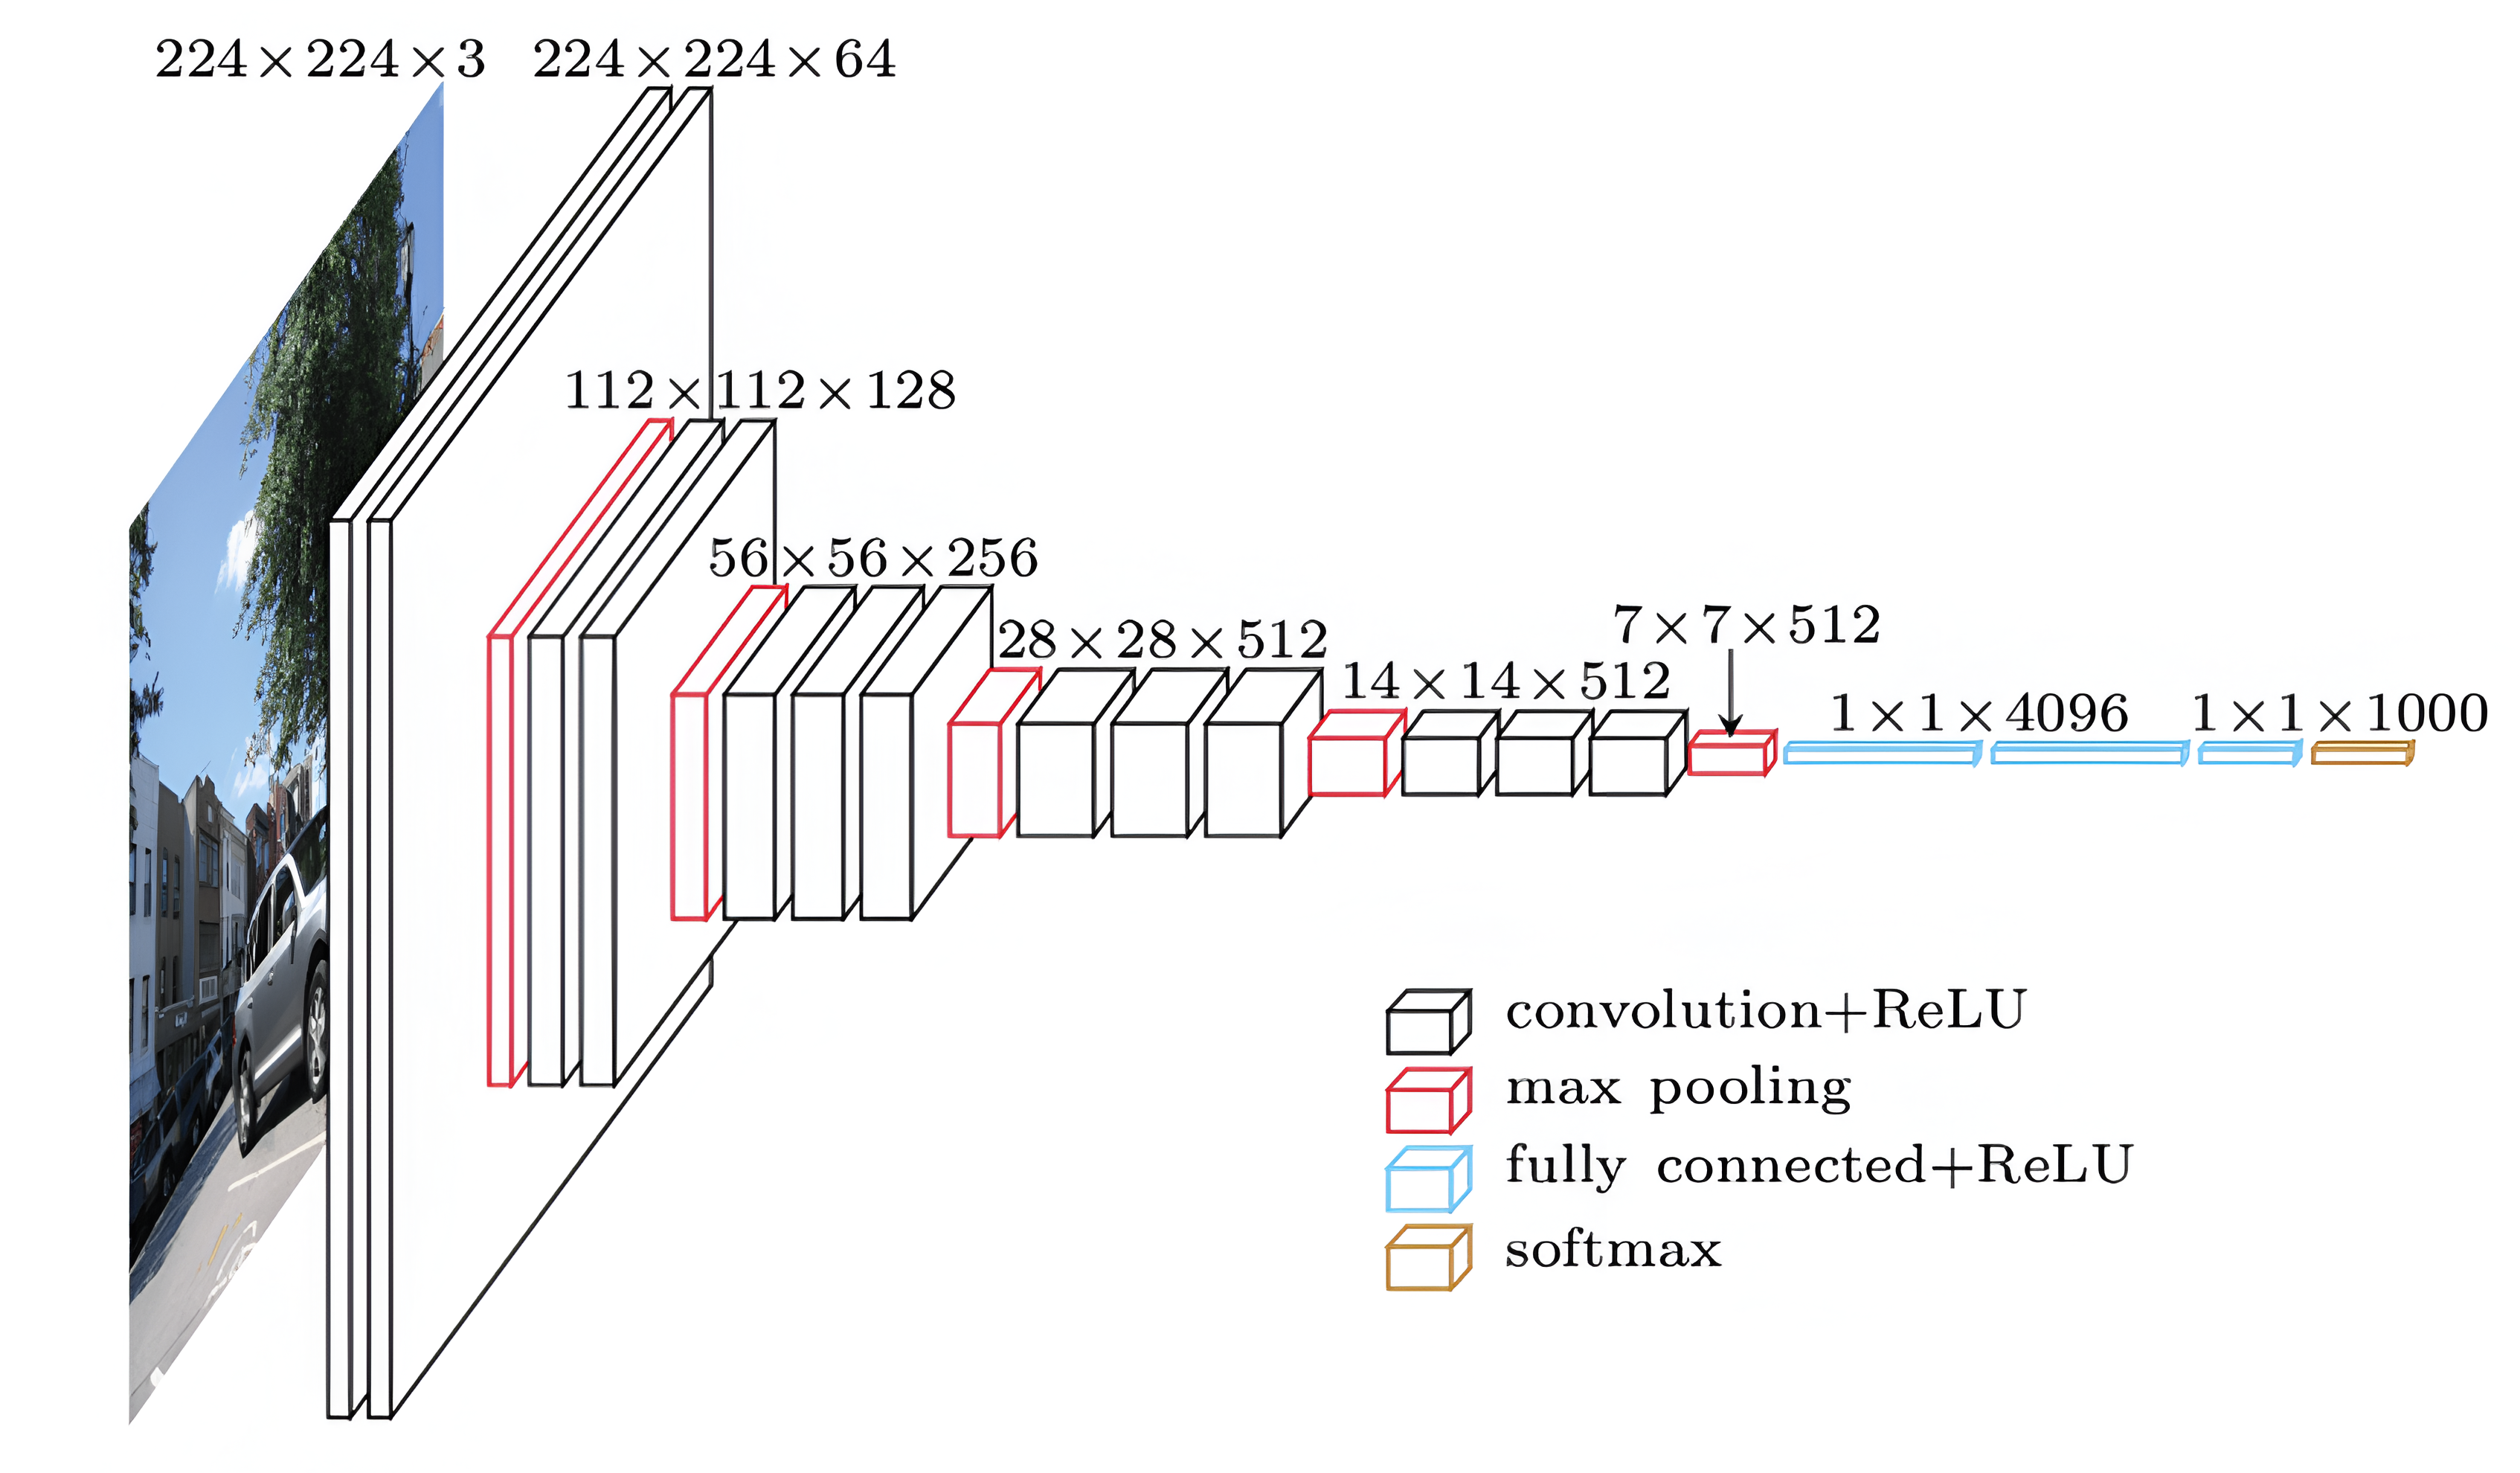
\includegraphics[scale=0.1]{imagenes/cap4/vgg-16.png}
	\caption[Arquitectura de la red VGG-16.]{Arquitectura de la red VGG-16. Las dimensiones se muestran en formato: Columnas x Filas x Canales \cite{66}.}
	\label{fig26}
\end{figure}

El uso de convoluciones 3x3 tiene dos ventajas:

\begin{itemize}
	\item Permite aplicar más convoluciones e incrementar la profundidad de la red al tener menos parámetros entrenables.
	\item Combinando las pequeñas convoluciones y la profundidad de la red, se pueden detectar características a pequeña escala, mientras que la agregación de escalas mayores va implícita al pasar de capa.
\end{itemize}

El uso de esta red se justifica por su sencillez y su capacidad para aprender características significativas de las imágenes mediante el bloque de capas convolucionales. 

En FacialSCDnet+, se ha modificado la estructura de la red de manera que se conserva la extracción de características a través de los bloques convolucionales, aprovechando los pesos preentrenados en ImageNet, mientras que en la parte final de la red se incluyen dos capas fully connected con 4096 neuronas cada una, junto con una capa de salida con una sola neurona para abordar el problema de regresión. Se realiza un proceso de fine-tuning, es decir, los pesos de los bloques convolucionales permanecen congelados, mientras que la parte final de la red es entrenada desde cero. En total, la red cuenta con 119,545,857 parámetros para el entrenamiento.

Dado su alto número de parámetros a entrenar, VGG-16 demanda recursos computacionales significativos, sin embargo, su gran rendimiento lo convierte en una opción atractiva para este trabajo.

\chapter{Experimentos}
\thispagestyle{empty}

\section{Entorno de desarrollo}

El proyecto se llevó a cabo utilizando exclusivamente el lenguaje de programación \textit{Python} en su versión 3.11.8, debido a su versatilidad y eficacia en diversas áreas, desde el renderizado de modelos 3D en \textit{Blender} hasta el desarrollo de modelos de aprendizaje profundo. Se emplearon diversas bibliotecas para diferentes tareas: \textit{Trimesh} y \textit{PyVista} junto con \textit{VTK} para la manipulación de modelos 3D; \textit{Mediapipe} para la extracción de puntos de referencia faciales; \textit{NumPy} y \textit{pandas} para el procesamiento de datos; \textit{PIL} para el trabajo con imágenes; \textit{matplotlib} y \textit{Seaborn} para la generación de gráficos; \textit{Optuna} para la optimización de hiperparámetros; \textit{MLflow} para la gestión de experimentos; y, finalmente, \textit{PyTorch} en su versión 2.0.1 junto con las librerías CUDA para el entrenamiento de modelos de aprendizaje profundo.

Con el objetivo de realizar un control de versiones durante el desarrollo del proyecto, se utilizó Git junto con GitHub. El código generado se puede encontrar en el siguiente enlace \url{https://github.com/ivansalinasugr/TFG}. Para más información, consultar el Readme del repositorio.

\section{Entorno de ejecución}

El proceso de ejecución se lleva a cabo en un entorno de alto rendimiento ubicado en la Universidad de Granada, al que se accede de forma remota a través de SSH. Se emplea un script de Shell para configurar los parámetros esenciales de los archivos. Por un lado, se utiliza SLURM para reservar recursos en la partición \enquote*{dios} del clúster, asignando una GPU del nodo \enquote*{dionisio}. Este nodo cuenta con dos Quadro RTX 8000, una memoria RAM de 512 GB DDR4 y dos procesadores Intel Xeon Silver 4216. Por otro lado, Conda se encarga de gestionar el entorno de software, garantizando la disponibilidad de las bibliotecas necesarias durante el proceso.

\section{Resultados}

En este trabajo se realizarán varios experimentos para entrenar y validar los dos modelos de aprendizaje presentados en FacialSCDnet+. Antes de los entrenamientos, se llevará a cabo un ajuste de parámetros para optimizar el rendimiento de los modelos. Finalmente, se compararán los resultados obtenidos con los obtenidos por FacialSCDnet. Estas comparaciones se efectuarán mediante el rendimiento en dos conjuntos de imágenes: el conjunto de test sintético de FacialSCDnet+, y el conjunto real de FacialSCDnet. Esto nos permitirá evaluar la robustez y la capacidad de generalización de los modelos propuestos.

El objetivo de estos experimentos es validar la hipótesis de que los modelos presentados en este trabajo pueden igualar o superar el rendimiento del modelo de referencia y por tanto, estimar mejor la SCD en fotografías faciales. A continuación, se presentan los detalles específicos y los resultados de estos experimentos.

\subsection{Ajuste de hiperparámetros}

Inicialmente, se llevó a cabo una fase de ajuste de hiperparámetros con el fin de determinar una configuración óptima para las arquitecturas propuestas. Los rangos de valores y los parámetros finales se detallan en la Tabla \ref{hipertuneo}. Además de los hiperparámetros mencionados, se estableció un entrenamiento a lo largo de 300 épocas, con una tasa de aprendizaje mínima de $10^{-12}$ y una reducción de la tasa de aprendizaje del 20\% cada 3 épocas consecutivas sin mejoras (paciencia), hasta un mínimo de $10^{-12}$.

\begin{table}[h]
	\centering
	\resizebox{\textwidth}{!}{%
	\begin{tabular}{llll}
	\hline
	Parámetros & Opciones & Mejor VGG-16 & Mejor ResNet-50 \\ \hline
	Optimizador & [adam, sgd] & adam & adam \\
	Tasa de aprendizaje & [$10^{-6}$, $10^{-3}$] & $4.63 \cdot 10^{-5}$ & 0.00042 \\
	Tamaño del lote & [16, 32, 64, 128] & 32 & 32 \\
	Paciencia & [2, 3, 4] & 3 & 3 \\
	\textit{Early Stopping} & [4, 6, 8] & 6 & 6 \\
	\textit{Dropout} (\%) & [0, 10, 20, 30] & 0 & 0 \\ \hline
	\end{tabular}%
	}
	\caption[Selección de parámetros de entrenamiento FacialSCDnet+.]{Parámetros de entrenamiento seleccionados para las redes VGG-16 y ResNet-50, junto a los rangos de valores utilizados durante el proceso de optimización de hiperparámetros.}
	\label{hipertuneo}
\end{table}

Los detalles de implementación de este tuneo de hiperparámetros se pueden observar en la Sección \ref{sec-hipertuneo}.

\subsection{Comparativa Arquitecturas}

A continuación, para valorar el comportamiento de las diferentes arquitecturas propuestas, compararemos los resultados obtenidos para FacialSCDnet+ usando el conjunto de validación. La Figura \ref{fig30} muestra la gráfica de la función de pérdida durante el entrenamiento de ambas arquitecturas, mientras que la Tabla \ref{val-metrics} muestra los valores finales de las métricas en el conjunto de entrenamiento de validación tras finalizar el entrenamiento.

\begin{figure}[h]
	\centering
	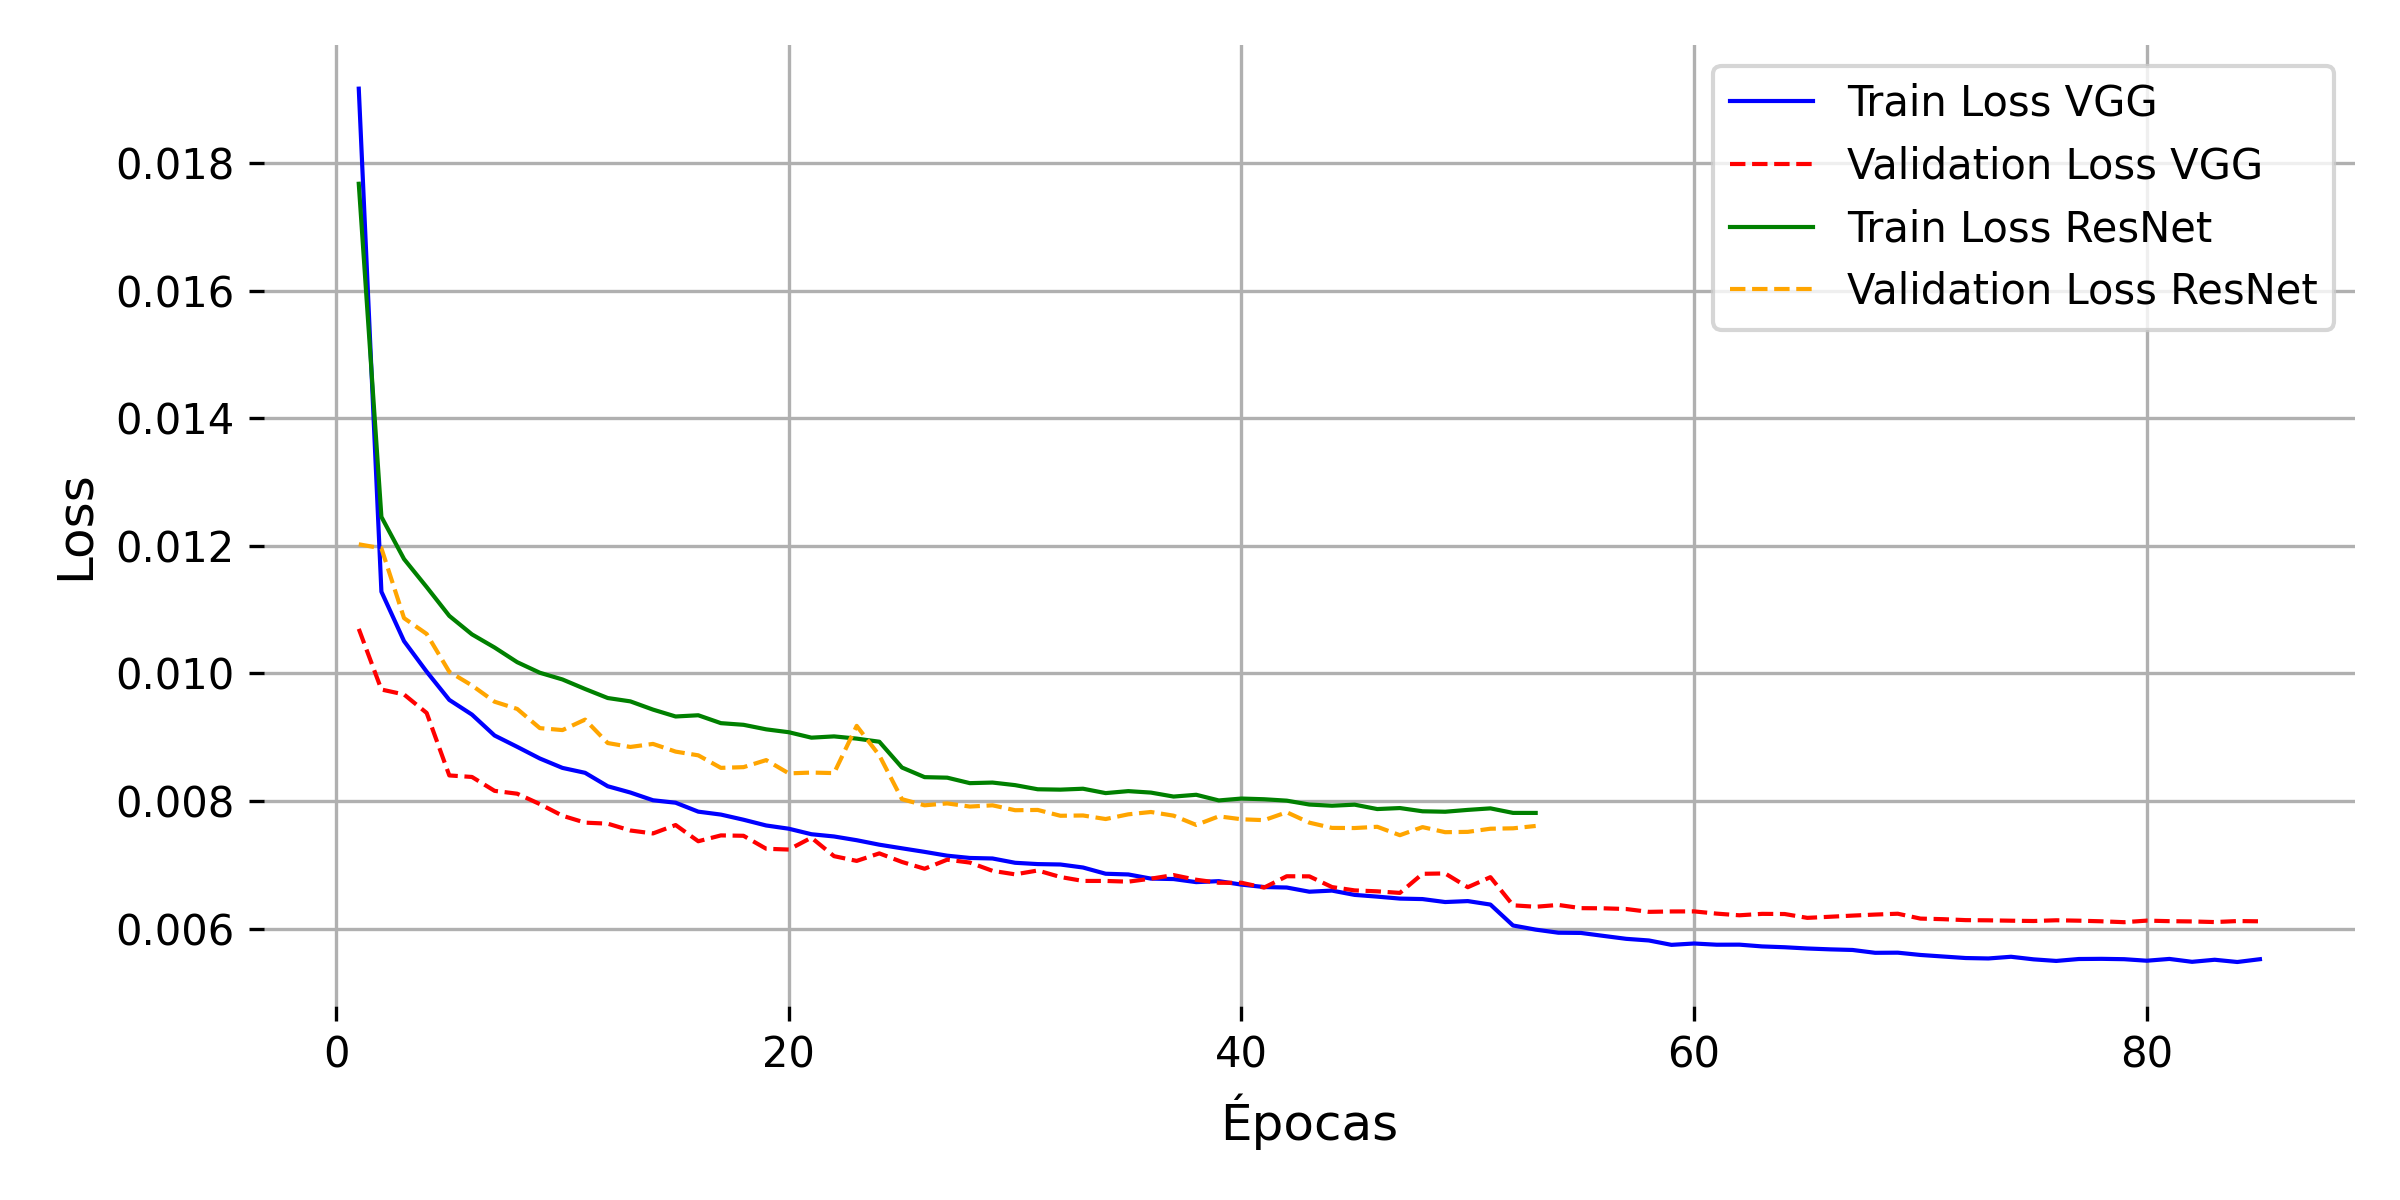
\includegraphics[scale=0.6]{imagenes/cap5/train_val_loss.png}
	\caption[Gráfica de pérdida en entrenamiento y validación.]{Gráfica de la función de pérdida durante el entrenamiento de las redes VGG-16 y ResNet-50. Para la red VGG se representa en azul la pérdida en el conjunto de entrenamiento mientras que en rojo se representa la pérdida en el conjunto de validación. Para la red ResNet se representa en verde la pérdida en el conjunto de entrenamiento mientras que en naranja se representa la pérdida en el conjunto de validación.}
	\label{fig30}
\end{figure}

Ambas arquitecturas comienzan con una pérdida alta que disminuye rápidamente durante las primeras épocas, lo cual es esperado ya que los modelos empiezan a ajustarse a los datos de entrenamiento. A medida que avanza el entrenamiento, ambos modelos van aprendiendo de los datos y por tanto, las pérdidas de entrenamiento y de validación siguen disminuyendo. 

VGG-16 muestra una convergencia más suave y una pérdida más baja tanto en entrenamiento como en validación en comparación con ResNet-50. Aunque ResNet-50 comienza bien, alcanza una meseta en la reducción de la pérdida de entrenamiento más rápidamente que VGG-16. Por tanto, la arquitectura VGG-16 tiene un mejor rendimiento en términos de pérdida tanto en entrenamiento como en validación en comparación con ResNet-50. 

Además, ambas arquitecturas finalizan el entrenamiento debido al \textit{early stopping}, tras seis épocas sin mejorar. La aplicación de esta técnica parece haber sido efectiva, ya que no se observa una gran divergencia entre las pérdidas de entrenamiento y validación hacia el final de la gráfica. Esto indica que los modelos no están sobreajustando significativamente y mantienen un buen equilibrio entre el ajuste a los datos de entrenamiento y la capacidad de generalización.

\begin{table}[h]
	\centering
	\resizebox{\textwidth}{!}{%
	\begin{tabular}{llll}
	\hline
	Métricas de evaluación &  & Validación VGG-16 & Validación ResNet-50 \\ \hline
	Distorsión (\%) &
	  \begin{tabular}[c]{@{}l@{}}Media (std)\\ Mediana\\ Perc 90, 95, 99\end{tabular} &
	  \begin{tabular}[c]{@{}l@{}}\textbf{0.61} (\textbf{0.614})\\ \textbf{0.434}\\ {[}\textbf{1.356}, \textbf{1.747}, \textbf{2.742}{]}\end{tabular} &
	  \begin{tabular}[c]{@{}l@{}}0.746 (0.722)\\ 0.532\\ {[}1.692, 2.176, 3.266{]}\end{tabular} \\ \hline
	MAE (cm) &
	  \begin{tabular}[c]{@{}l@{}}Media (std)\\ Mediana\\ Perc 90, 95, 99\end{tabular} &
	  \begin{tabular}[c]{@{}l@{}}\textbf{31.425} (44.048)\\ \textbf{12.194}\\ {[}\textbf{89.95}, \textbf{125.106}, 204.385{]}\end{tabular} &
	  \begin{tabular}[c]{@{}l@{}}34.072 (\textbf{43.447})\\ 15.597\\ {[}93.849, 126.878, \textbf{194.479}{]}\end{tabular} \\ \hline
	MRE (\%) &
	  \begin{tabular}[c]{@{}l@{}}Media (std)\\ Mediana\\ Perc 90, 95, 99\end{tabular} &
	  \begin{tabular}[c]{@{}l@{}}\textbf{0.111} (0.138)\\ \textbf{0.075}\\ {[}\textbf{0.233}, \textbf{0.328}, \textbf{0.647}{]}\end{tabular} &
	  \begin{tabular}[c]{@{}l@{}}0.128 (\textbf{0.137})\\ 0.093\\ {[}0.266, 0.356, 0.659{]}\end{tabular} \\ \hline
	R$^2$ &
	  &
	  \textbf{0.897} &
	  0.894 \\ \hline
	\end{tabular}%
	}
	\caption[Métricas en validación VGG-16 y ResNet-50.]{Métricas en el conjunto de validación tras el proceso de entrenamiento de las redes VGG-16 y ResNet-50.}
	\label{val-metrics}
\end{table}

A pesar de que los valores del MAE son relativamente altos, ambos modelos muestran un error medio de distorsión menor al 1\% y un error relativo medio muy bajo, lo cual es un valor aceptable para que la predicción sea fiable. En este contexto, VGG-16 presenta una distorsión ligeramente más baja que ResNet-50, lo que indica una mejor predicción de las distancias.

En general, aunque ambos modelos tienen buenos resultados, sobre todo en términos de distorsión, VGG-16 destaca con mejor rendimiento que ResNet-50 en todas las métricas.

\subsection{Comparativa con el estado del arte: FacialSCDnet}

En esta sección se lleva a cabo una comparativa entre los tres modelos utilizados para la estimación de la SCD: VGG-16 y ResNet-50 de FacialSCDnet+ y VGG-16 de FacialSCDnet. Para ello, se evalúan los modelos en dos conjuntos de datos: el conjunto de test sintético propuesto en este trabajo, previamente definido en la Sección \ref{protocolo} y un conjunto de test de imágenes reales propuesto en \cite{14}. Así, se pretende proporcionar una comparativa en igualdad de condiciones para ambos métodos. 

Aunque no se deberían utilizar los conjuntos de test para tomar decisiones metodológicas debido al riesgo de \textit{data snooping} (lo que puede llevar a un sobreajuste a los datos de test), en este trabajo seguiremos el protocolo del estudio de referencia \cite{14} y de muchos otros estudios, utilizando los conjuntos de test para evaluar y comparar el rendimiento de los modelos.

Para hacer la comparación más visual, se complementarán las métricas con figuras que muestren las predicciones comparadas con los valores objetivo, así como los errores de predicción representados en diagramas de caja.

\subsubsection{Test imágenes sintéticas}

Este conjunto de datos contiene 28 935 imágenes sintéticas en 35 distancias desde 50 a 600 cm. Los resultados de evaluar los modelos en este conjunto de datos se muestran en la Tabla \ref{test-mio}.

\begin{table}[h]
	\centering
	\resizebox{\textwidth}{!}{%
	\begin{tabular}{lllll}
	\hline
	\begin{tabular}[c]{@{}l@{}}Métricas de \\ evaluación\end{tabular} &
	&
	\begin{tabular}[c]{@{}l@{}}VGG-16 \\ FSCDnet\end{tabular} &
	\begin{tabular}[c]{@{}l@{}}VGG-16 \\ FSCDnet+\end{tabular} &
	\begin{tabular}[c]{@{}l@{}}ResNet-50 \\ FSCDnet+\end{tabular} \\ \hline
	Distorsión (\%) &
	\begin{tabular}[c]{@{}l@{}}Media (std)\\ Mediana\\ Perc 90, 95, 99\end{tabular} &
	\begin{tabular}[c]{@{}l@{}}1.218 (1.395)\\ 0.764\\ {[}2.878, 3.893, 6.826{]}\end{tabular} &
	\begin{tabular}[c]{@{}l@{}}\textbf{0.624} (\textbf{0.596})\\ \textbf{0.453}\\ {[}\textbf{1.381}, \textbf{1.758}, \textbf{2.639}{]}\end{tabular} &
	\begin{tabular}[c]{@{}l@{}}0.781 (0.754)\\ 0.55\\ {[}1.782, 2.265, 3.445{]}\end{tabular} \\ \hline
	MAE (cm) &
	\begin{tabular}[c]{@{}l@{}}Media (std)\\ Mediana\\ Perc 90, 95, 99\end{tabular} &
	\begin{tabular}[c]{@{}l@{}}53.237 (73.434)\\ 21.594\\ {[}147.604, 220.045, 338.481{]}\end{tabular} &
	\begin{tabular}[c]{@{}l@{}}\textbf{32.165} (44.045)\\ \textbf{12.771}\\ {[}\textbf{92.037}, \textbf{127.188}, 200.073{]}\end{tabular} &
	\begin{tabular}[c]{@{}l@{}}35.095 (\textbf{43.954})\\ 16.498\\ {[}96.793, 130.566, \textbf{193.916}{]}\end{tabular} \\ \hline
	MRE (\%) &
	\begin{tabular}[c]{@{}l@{}}Media (std)\\ Mediana\\ Perc 90, 95, 99\end{tabular} &
	\begin{tabular}[c]{@{}l@{}}0.215 (0.299)\\ 0.132\\ {[}0.455, 0.681, 1.567{]}\end{tabular} &
	\begin{tabular}[c]{@{}l@{}}\textbf{0.113} (\textbf{0.135})\\ \textbf{0.078}\\ {[}\textbf{0.24}, \textbf{0.327}, \textbf{0.64}{]}\end{tabular} &
	\begin{tabular}[c]{@{}l@{}}0.133 (0.14)\\ 0.099\\ {[}0.277, 0.362, 0.669{]}\end{tabular} \\ \hline
	R$^2$ &
	&
	0.673 &
	\textbf{0.895} &
	0.89 \\ \hline
	\end{tabular}%
	}
	\caption[Métricas en el conjunto de test sintético.]{Métricas en el conjunto de test sintético de FacialSCDnet+, comparando los modelos VGG-16 y ResNet-50 de FacialSCDnet+ contra el modelo de FacialSCDnet.}
	\label{test-mio}
\end{table}

Esta tabla refleja cómo VGG-16 FacialSCDnet+ presenta mejores resultados en la mayoría de las métricas, seguido por ResNet-50 FacialSCDnet+ y VGG-16 FacialSCDnet. Estos resultados sugieren que el método FacialSCDnet+ proporciona una mejora significativa en el rendimiento de la predicción en comparación con el método FacialSCDnet, y se reafirma la conclusión obtenida en la comparativa anterior, donde la arquitectura de VGG-16 se comporta mejor que ResNet-50 en este contexto específico.

Ambos modelos de FacialSCDnet+ presentan una distorsión inferior al 1\%, lo cual se considera un margen de error aceptable, incluso a pesar de que muestran un MAE elevado. Visualmente, podemos analizar la distribución del error en la Figura \ref{fig33}, donde se compara el error en las predicciones mediante gráficos de caja.

\begin{figure}[h]
	\centering
	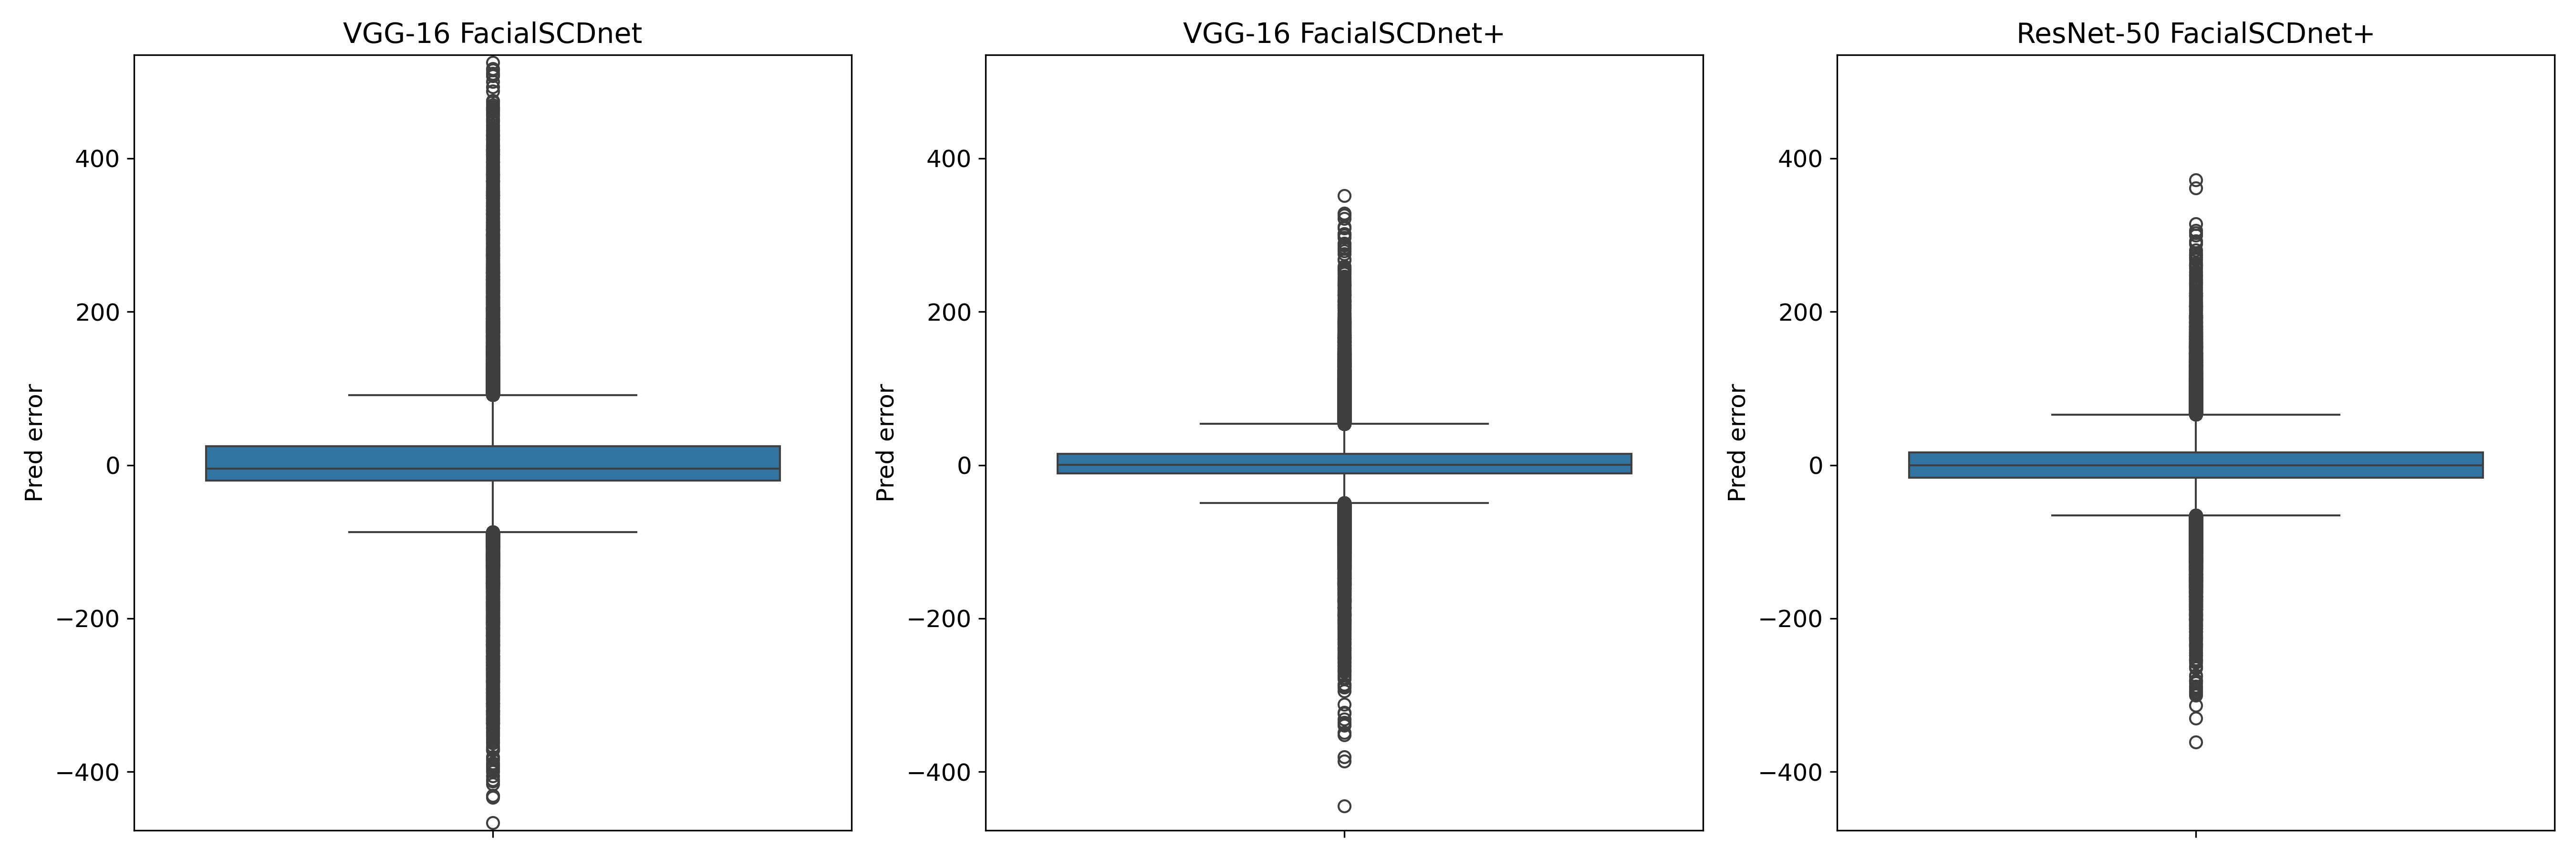
\includegraphics[width=\textwidth]{imagenes/cap5/boxplot_own.png}
	\caption[Comparación predicciones de error test sintético.]{Gráfica que muestra la comparación de las predicciones de error para cada uno de los 3 modelos utilizados.}
	\label{fig33}
\end{figure}

En estas gráficas se puede observar cómo VGG-16 FacialSCDnet muestra la mayor variabilidad y la mayor cantidad de outliers, lo que sugiere que este modelo enfrenta más dificultades para hacer predicciones precisas en muchos casos. Los dos modelos de FacialSCDnet+ mejoran en comparación con FacialSCDnet, reduciendo tanto la variabilidad como la cantidad de outliers, lo que indica un desempeño más consistente. En particular, el modelo VGG-16 FacialSCDnet+ parece tener menor variabilidad, mientras que ResNet-50 presenta la menor cantidad de outliers.

En la Figura \ref{fig36} se pueden observar predicciones de la distancia para algunas de las imágenes del conjunto sintético.

\begin{figure}[h]
	\centering
	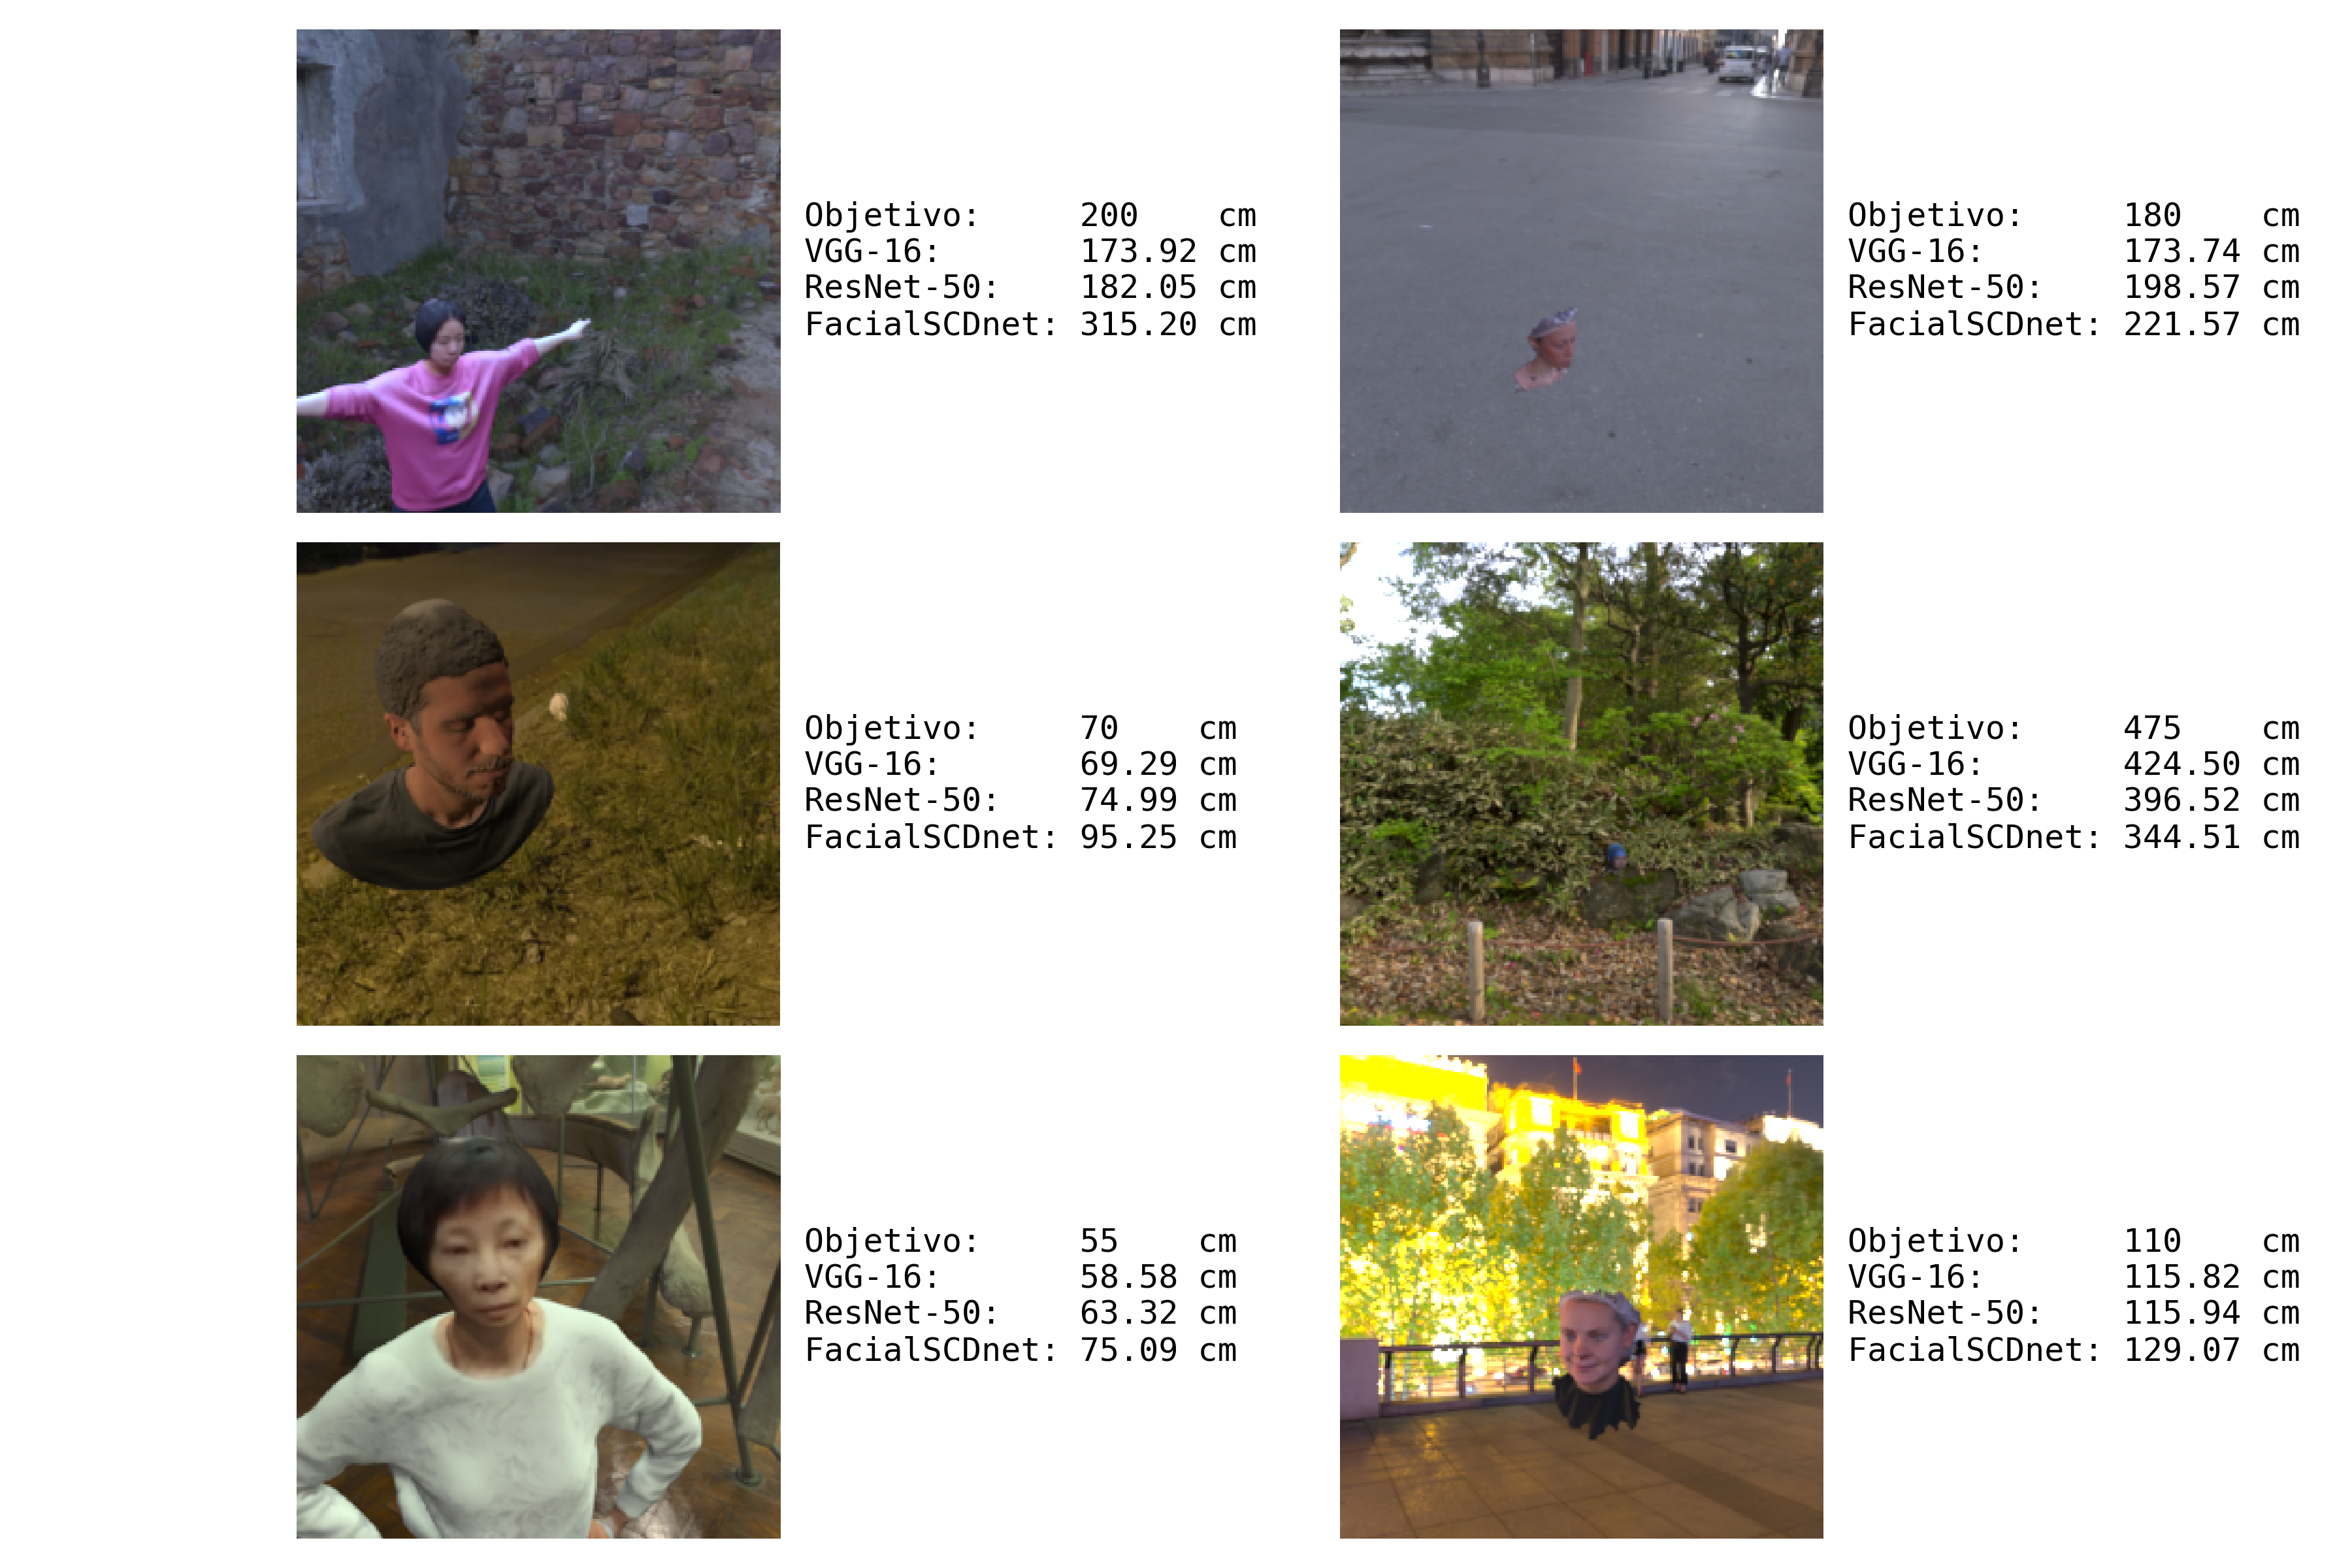
\includegraphics[width=\textwidth]{imagenes/cap5/predicts_own.png}
	\caption[Ejemplos de predicciones en imágenes sintéticas.]{Ejemplos de predicciones en imágenes sintéticas para los distintos modelos VGG-16 y ResNet-50 de FacialSCDnet+ y VGG-16 de FacialSCDnet.}
	\label{fig36}
\end{figure}

Es importante destacar que los modelos de FacialSCDnet+ parten con cierta ventaja en esta compartiva, ya que han sido entrenados en un conjunto similar al empleado en este test. Por esta razón, a continuación se evaluarán los modelos en un conjunto de test compuesto únicamente de imágenes reales.


\subsubsection{Test imágenes reales}

Este conjunto de datos contiene 1134 imágenes reales en 29 distancias desde 50 a 500 cm. Los resultados de evaluar los modelos en este conjunto de datos se muestran en la Tabla \ref{test-real}.

\begin{table}[h]
	\centering
	\resizebox{\textwidth}{!}{%
	\begin{tabular}{lllll}
	\hline
	\begin{tabular}[c]{@{}l@{}}Métricas de \\ evaluación\end{tabular} &
	&
	\begin{tabular}[c]{@{}l@{}}VGG-16 \\ FSCDnet\end{tabular} &
	\begin{tabular}[c]{@{}l@{}}VGG-16 \\ FSCDnet+\end{tabular} &
	\begin{tabular}[c]{@{}l@{}}ResNet-50 \\ FSCDnet+\end{tabular} \\ \hline
	Distorsión (\%) &
	\begin{tabular}[c]{@{}l@{}}Media (std)\\ Mediana\\ Perc 90, 95, 99\end{tabular} &
	\begin{tabular}[c]{@{}l@{}}1.233 (1.615)\\ 0.77\\ {[}3.005, 3.869, 8.389{]}\end{tabular} &
	\begin{tabular}[c]{@{}l@{}}\textbf{0.702} (\textbf{0.727})\\ \textbf{0.477}\\ {[}\textbf{1.637}, \textbf{2.195}, \textbf{3.459}{]}\end{tabular} &
	\begin{tabular}[c]{@{}l@{}}1.257 (0.993)\\ 1.085\\ {[}2.59, 3.136, 4.108{]}\end{tabular} \\ \hline
	MAE (cm) &
	\begin{tabular}[c]{@{}l@{}}Media (std)\\ Mediana\\ Perc 90, 95, 99\end{tabular} &
	\begin{tabular}[c]{@{}l@{}}31.594 (55.366)\\ 9.994\\ {[}98.136, 154.061, 288.525{]}\end{tabular} &
	\begin{tabular}[c]{@{}l@{}}\textbf{26.05} (\textbf{48.391})\\ \textbf{8.69}\\ {[}\textbf{71.072}, \textbf{117.413}, 261.572{]}\end{tabular} &
	\begin{tabular}[c]{@{}l@{}}39.852 (58.581)\\ 16.233\\ {[}130.143, 179.453, \textbf{257.784}{]}\end{tabular} \\ \hline
	MRE (\%) &
	\begin{tabular}[c]{@{}l@{}}Media (std)\\ Mediana\\ Perc 90, 95, 99\end{tabular} &
	\begin{tabular}[c]{@{}l@{}}0.187 (0.33)\\ 0.103\\ {[}0.409, 0.58, 1.61{]}\end{tabular} &
	\begin{tabular}[c]{@{}l@{}}\textbf{0.098} (\textbf{0.101})\\ \textbf{0.067}\\ {[}\textbf{0.212}, \textbf{0.3}, \textbf{0.523}{]}\end{tabular} &
	\begin{tabular}[c]{@{}l@{}}0.161 (0.126)\\ 0.137\\ {[}0.342, 0.409, \textbf{0.523}{]}\end{tabular} \\ \hline
	R$^2$ &
	&
	0.786 &
	\textbf{0.829} &
	0.624 \\ \hline
	\end{tabular}%
	}
	\caption[Métricas en el conjunto de test real.]{Métricas en el conjunto de test real de FacialSCDnet, comparando los modelos VGG-16 y ResNet-50 de FacialSCDnet+ contra el modelo de FacialSCDnet.}
	\label{test-real}
\end{table}

Esta tabla refleja cómo VGG-16 FacialSCDnet+ presenta mejores resultados en todas las métricas, seguido por ResNet-50 FacialSCDnet+ y VGG-16 FacialSCDnet. Esto sugiere que el método FacialSCDnet+ proporciona una mejora significativa en el rendimiento de la predicción en comparación con el método FacialSCDnet estándar, y que el modelo VGG-16 es más efectivo que el ResNet-50 en este contexto específico.

El modelo VGG-16 de FacialSCDnet+ es el único que presenta una distorsión inferior al 1\%. Aunque todavía tiene un MAE ligeramente alto, este nivel de error en la distorsión se considera aceptable.

En este contexto, es notable destacar un error cometido en el método FacialSCDnet. A la hora de evaluar el modelo con las imágenes reales, se les aplicaba una máscara para añadirles un fondo sintético. Esto provocaba que el rendimiento del modelo aumentara artificialmente, ya que la red neuronal internamente estaba aprendiendo a localizar a los individuos en fotografías lejanas gracias al preprocesamiento. Así, se estaba cometiendo un sesgo significativo debido a la aplicación de  máscaras. Los resultados pueden comprobarse en la publicación original \cite{14}, donde se muestran resultados que reducen una sexta parte del error real sin preprocesamiento.

La Figura \ref{fig35} muestra una comparación de las predicciones de error para los tres modelos utilizando gráficos de caja.

\begin{figure}[h]
	\centering
	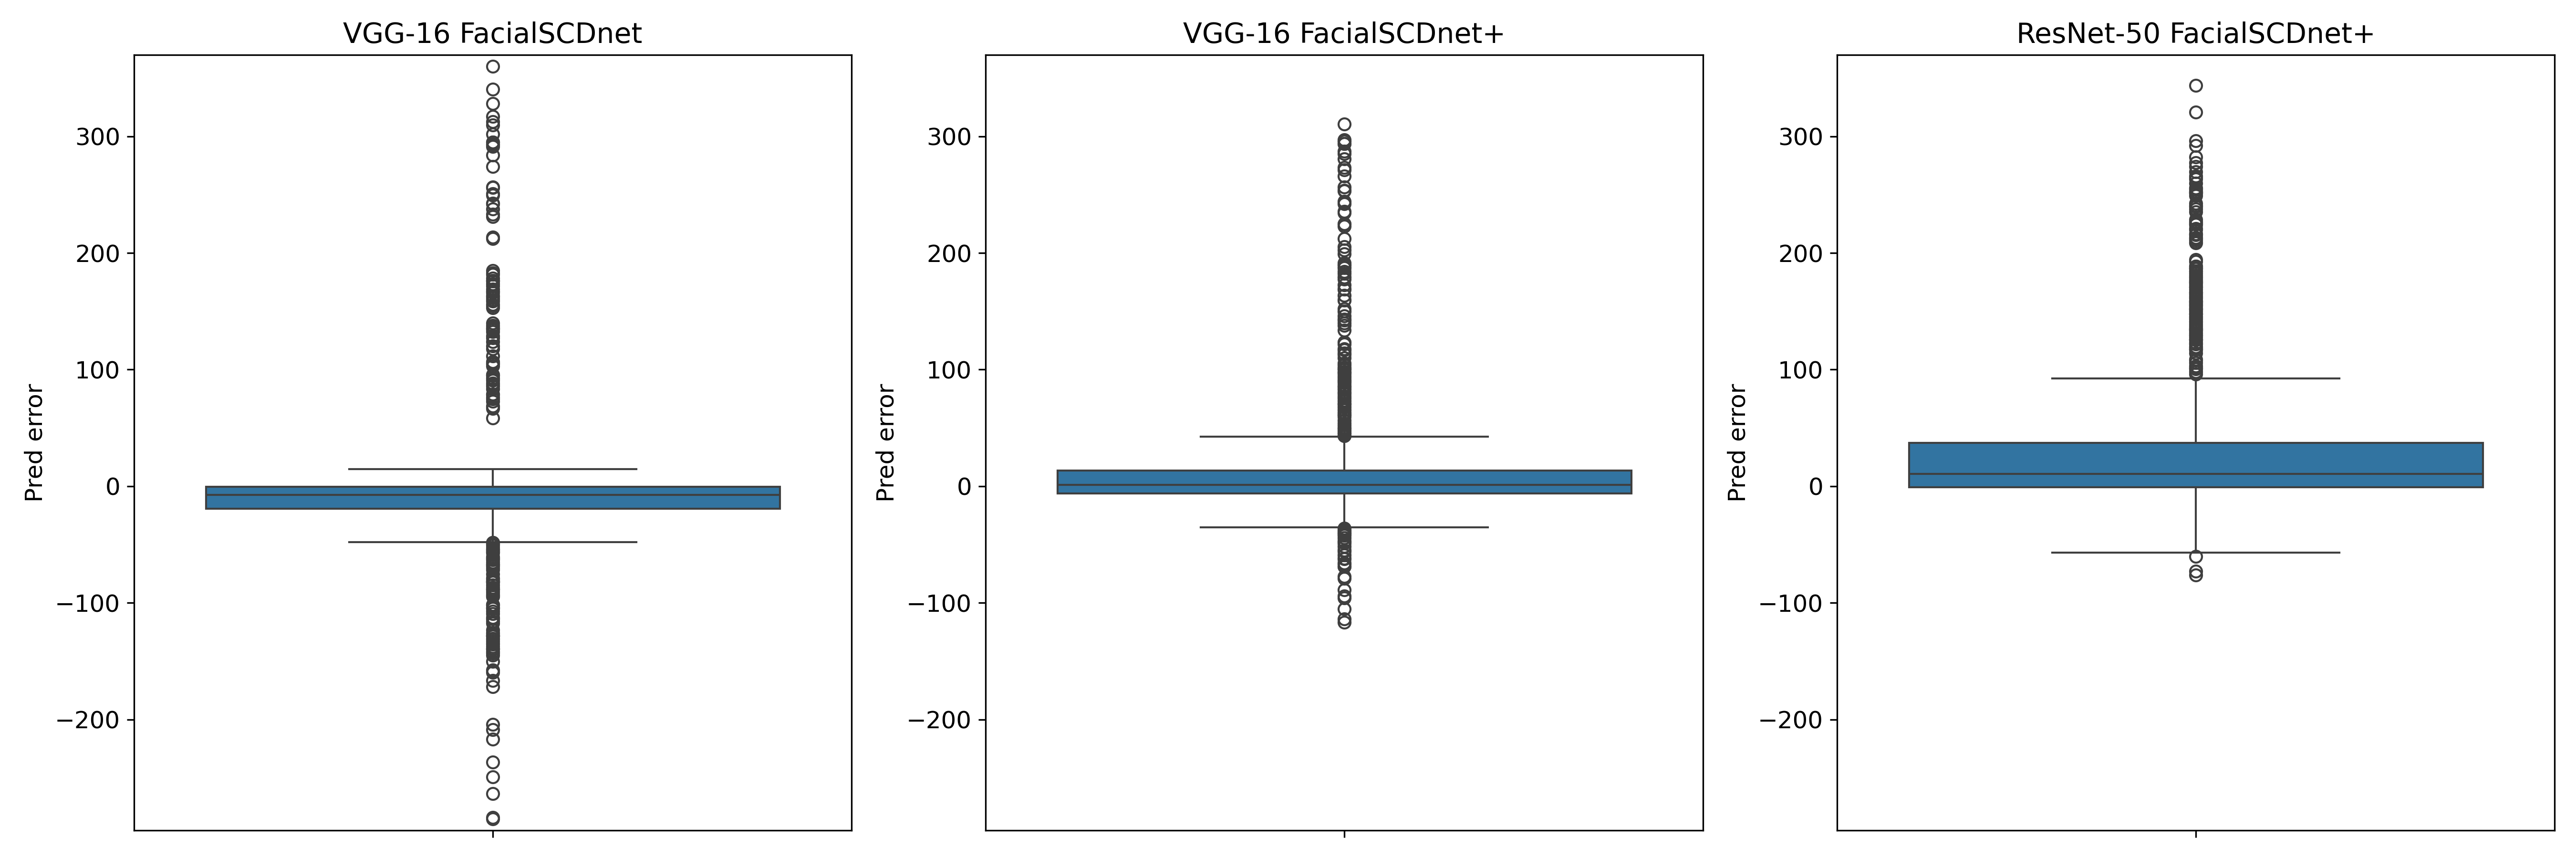
\includegraphics[width=\textwidth]{imagenes/cap5/boxplot_real.png}
	\caption[Comparación predicciones de error test real.]{Gráfica que muestra la comparación de las predicciones de error para cada uno de los 3 modelos utilizados.}
	\label{fig35}
\end{figure}

Se observa que VGG-16 FacialSCDnet presenta la mayor cantidad de outliers, lo que sugiere que este modelo tiene más dificultades para hacer predicciones precisas en ciertos casos. Además, este modelo tiende tanto a sobreestimar como a infraestimar las predicciones. Por otro lado, ambos modelos de FacialSCDnet+ muestran una menor cantidad de outliers, aunque tienen una mayor variabilidad, especialmente el ResNet-50 FacialSCDnet+. El modelo VGG-16 FacialSCDnet+, a pesar de tener una variabilidad ligeramente mayor que el VGG-16 FacialSCDnet, presenta menos outliers, lo cual sugiere que es el modelo más consistente de los presentados.

En la Figura \ref{fig37} se pueden observar predicciones de la distancia para algunas de las imágenes del conjunto real.

\begin{figure}[h]
	\centering
	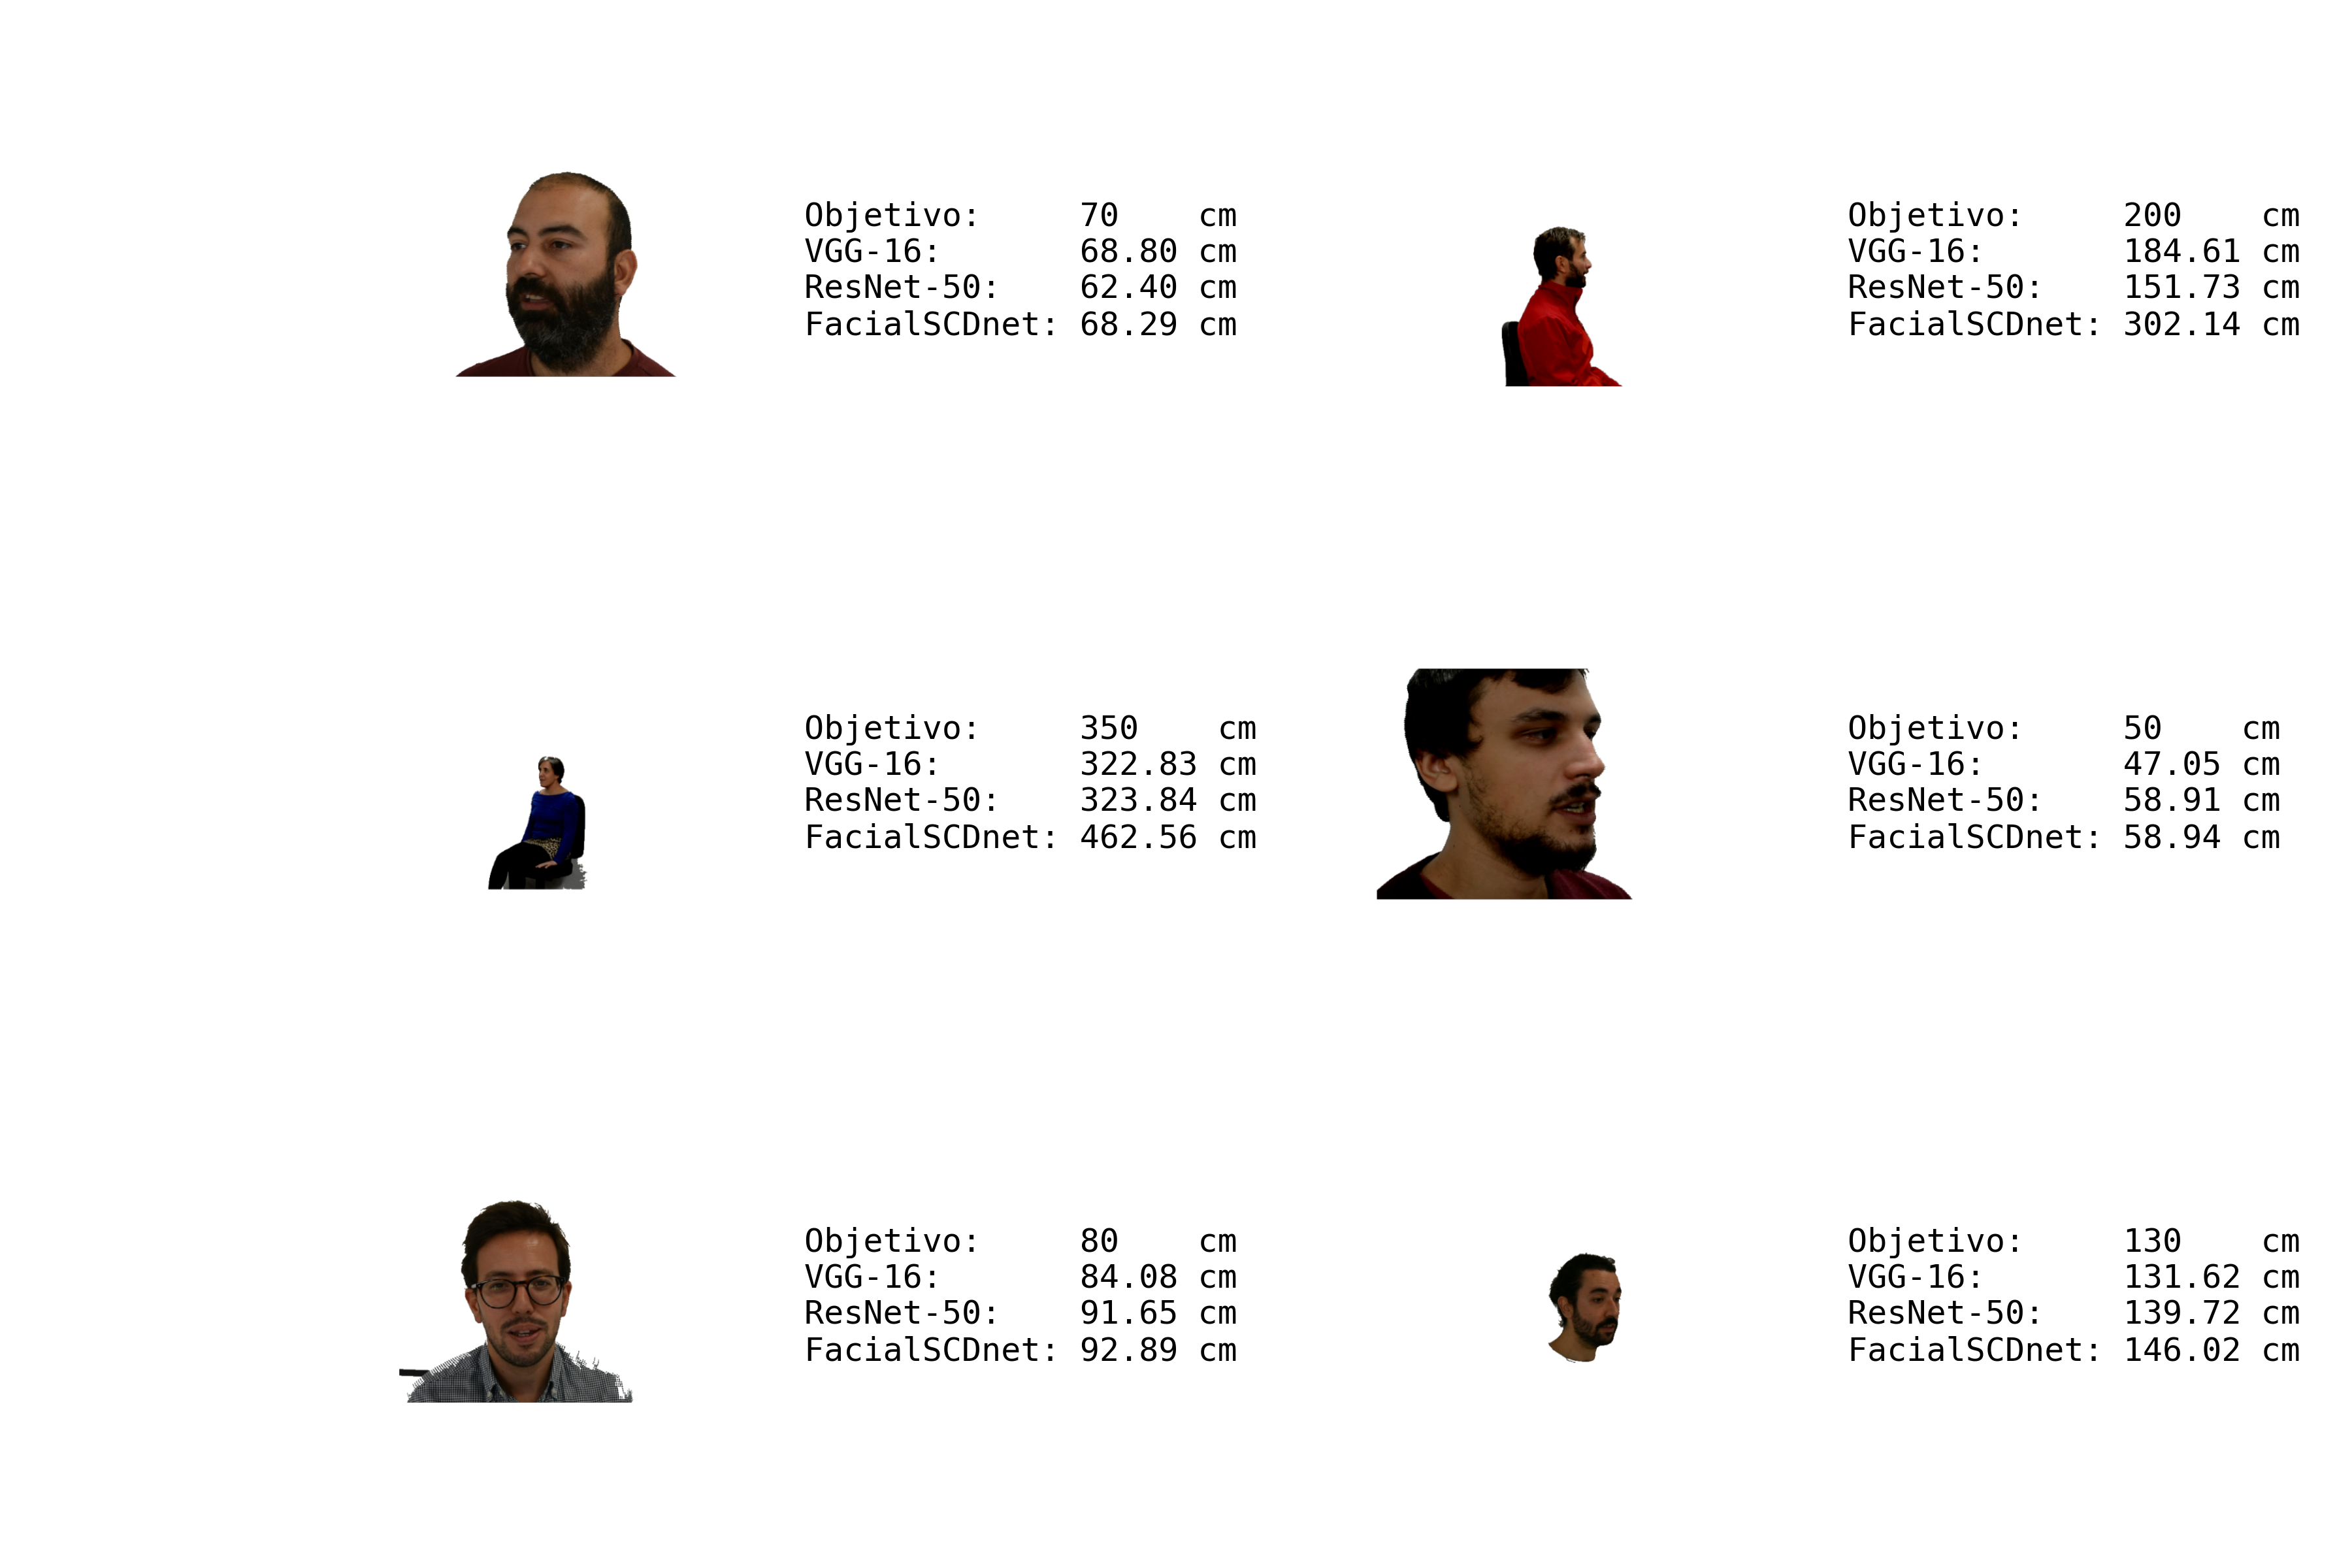
\includegraphics[width=\textwidth]{imagenes/cap5/predicts_real.png}
	\caption[Ejemplos de predicciones en imágenes reales.]{Ejemplos de predicciones en imágenes reales para los distintos modelos VGG-16 y ResNet-50 de FacialSCDnet+ y VGG-16 de FacialSCDnet.}
	\label{fig37}
\end{figure}

La Figura \ref{fig34} representa una comparativa del rendimiento de los métodos a la hora de prededir la SCD, de forma que podemos observar la dispersión concreta de las estimaciones con respecto a la SCD real. La primera fila muestra los resultados en test de los tres métodos comparados para el conjunto de imágenes sintético, mientras que la segunda fila muestra los resultados sobre el conjunto de imágenes reales. La principal diferencia entre ambos conjuntos de datos es evidente, el número de imágenes sintéticas que podemos generar permite cubrir un amplio rango de distancias en comparacion con las imágenes reales. Esto nos permite contextualizar el rendimiento de los modelos. 

\begin{figure}[h]
	\centering
	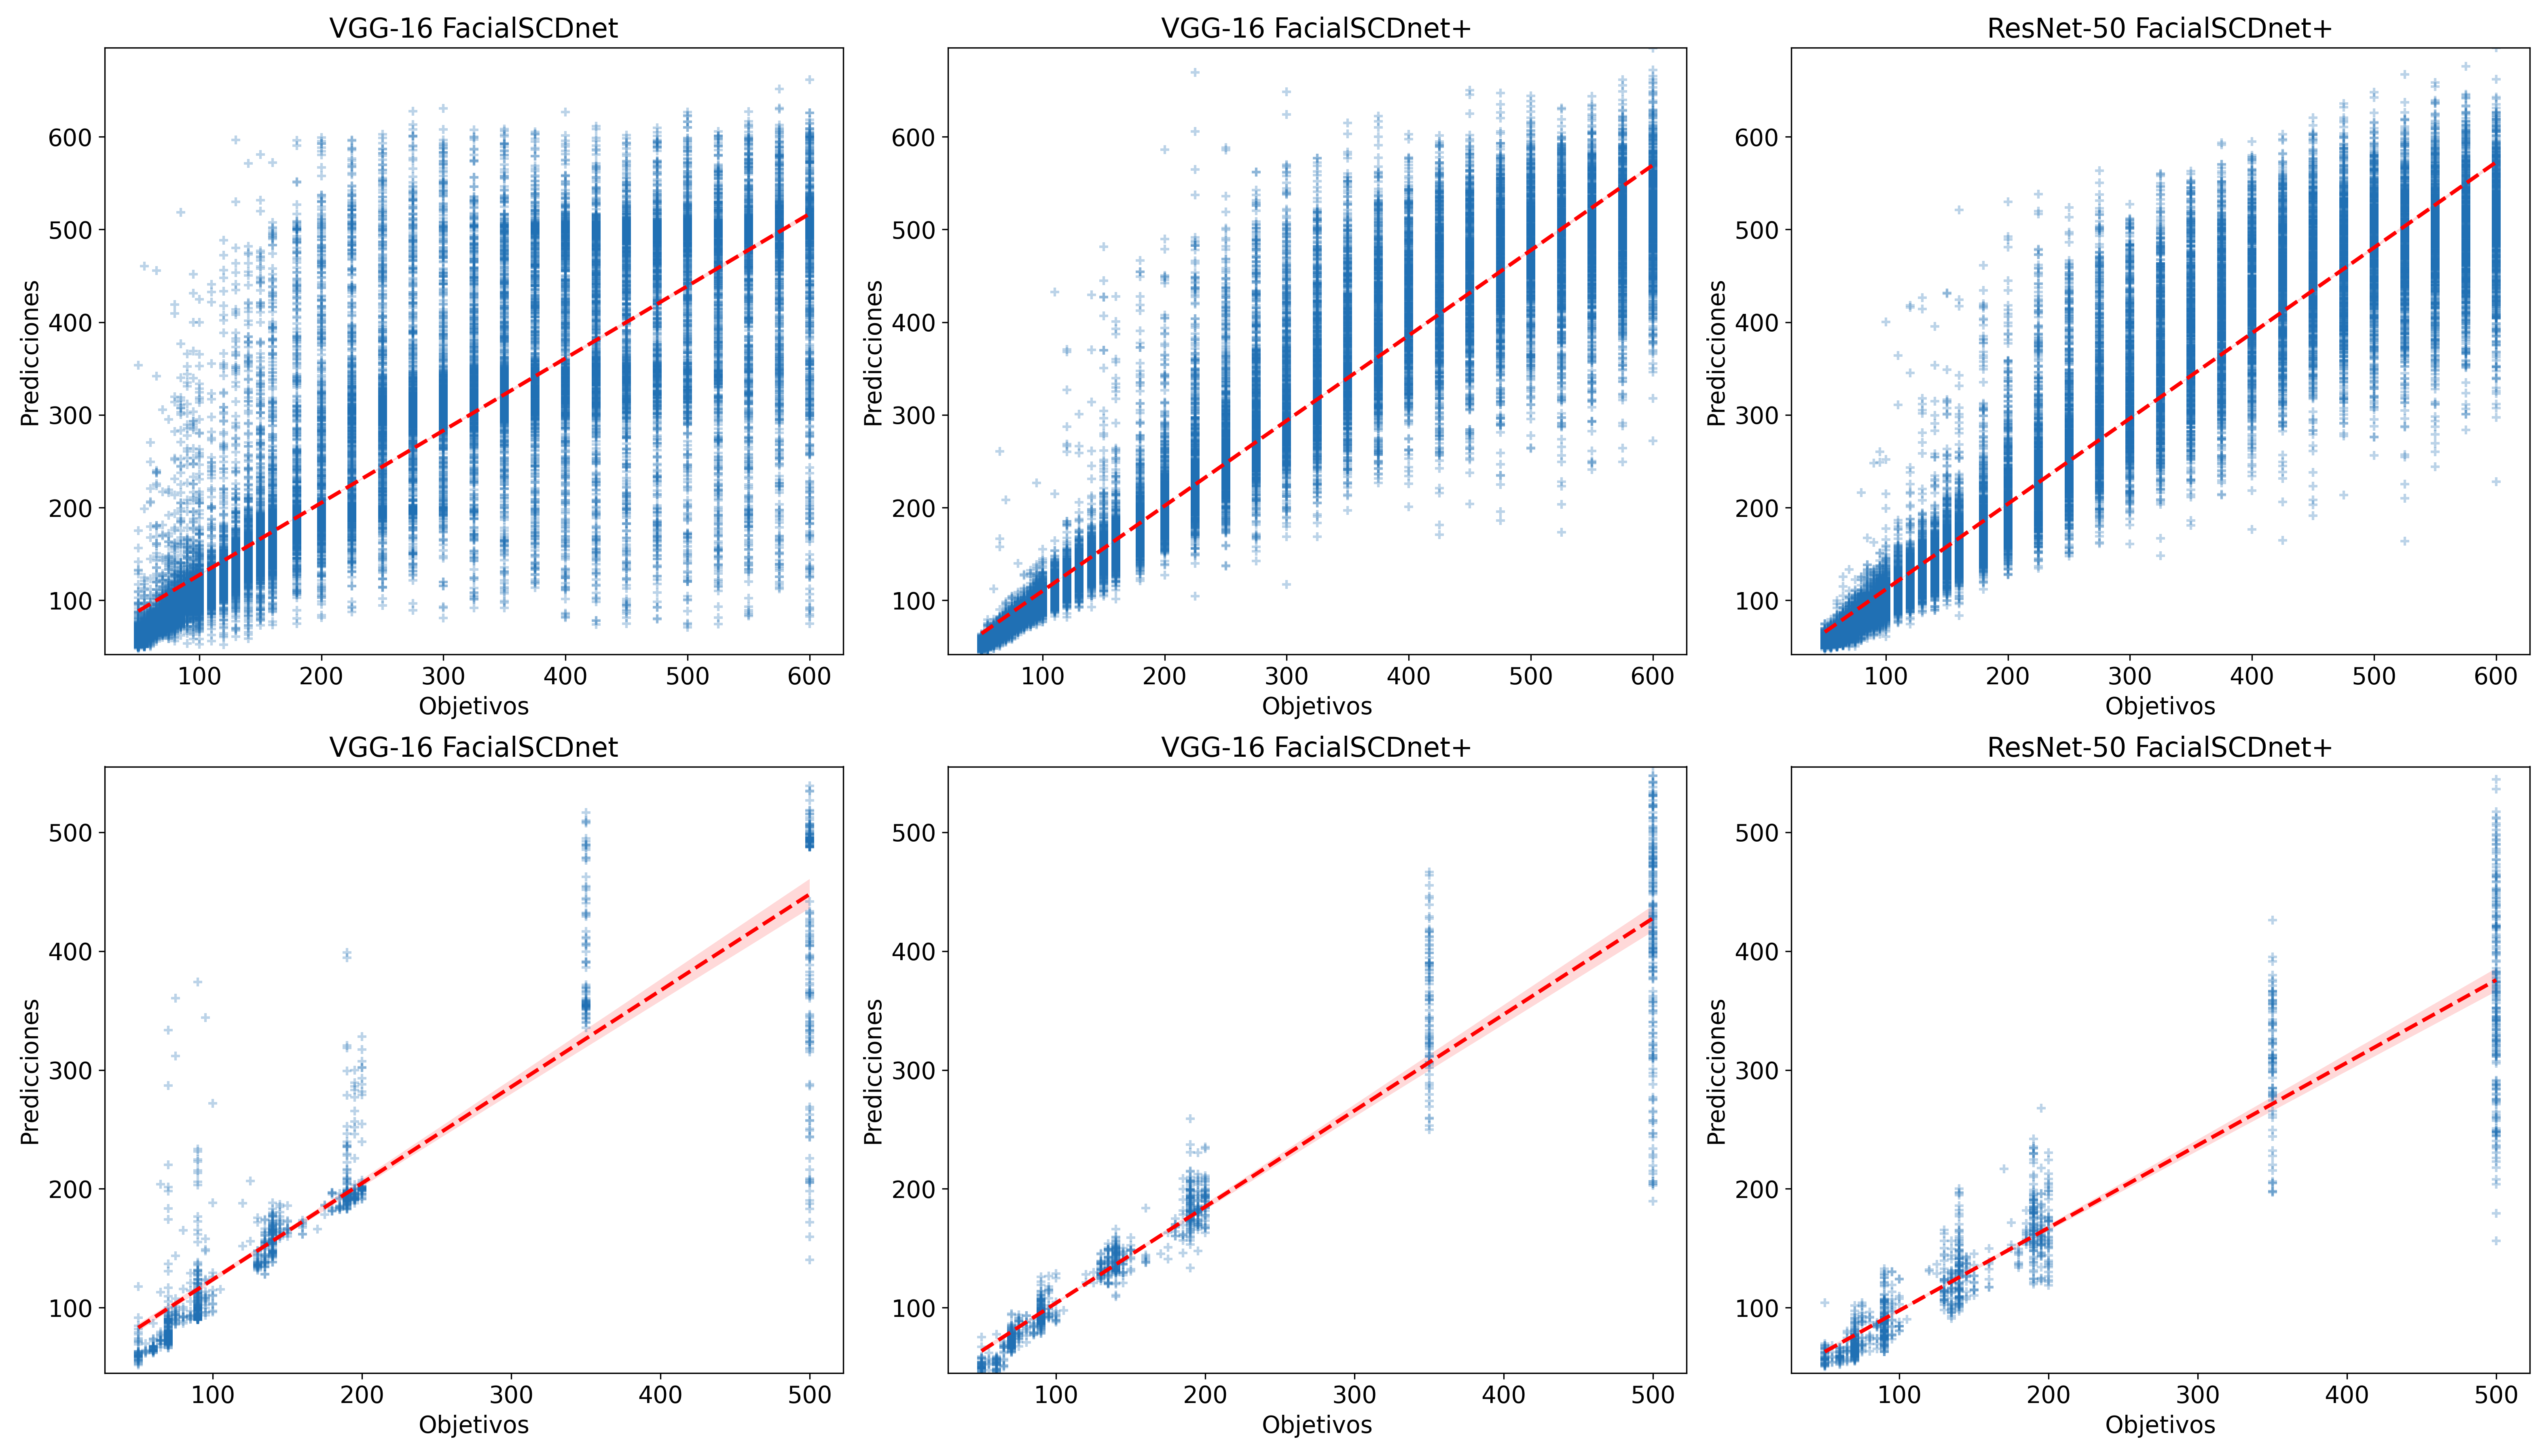
\includegraphics[width=\textwidth]{imagenes/cap5/comp_etiquetas.png}
	\caption[Comparación etiquetas de test.]{Gráfica comparativa de predicciones vs objetivos para los tres modelos utilizados. La primera fila presenta los resultados en el conjunto de test sintético, mientras que la segunda fila muestra los resultados en el conjunto de test real.}
	\label{fig34}
\end{figure}

En línea con los resultados cuantitativos mostrados en las Tablas \ref{test-mio} y \ref{test-real}, ambas arquitecturas de FacialSCDnet+ tienen un comportamiento similar, realizando estimaciones mucho más precisas a distancias cortas (en torno a 1.5 metros) y mostrando más variabilidad a distancias mayores. Es precisamente en esos casos donde el impacto de la distorsión de perspectiva es menos relevante, con lo que los resultados se explican al emplear la metrica de distorsión para guiar el entrenamiento del modelo. Para el conjunto de datos real se puede extraer una conclusión similar, destacando cómo el modelo basado en VGG-16 de FacialSCDnet+ parece minimizar la dispersión en la estimación de SCD, reduciendo los outliers y mostrando un comportamiento más consistente. En el caso del modelo de referencia, FacialSCDnet, la gráfica deja patente cómo el método, al no ser ayudado por la aplicación de las máscaras de transparencia, tiene un rendimiento real considerablemente peor al reportado en \cite{14} y del obtenido por FacialSCDnet+.

Además, los coeficientes de determinación R$^2$ (Tablas \ref{test-mio} y \ref{test-real}) proporcionan una medida cuantitativa adicional del rendimiento de los modelos, indicando qué tan bien se ajustan las líneas de regresión de la Figura \ref{fig34} a los datos. En concreto, el modelo VGG-16 de FacialSCDnet+ alcanza un valor de 0.895 para el conjunto de datos sintéticos, mientras que para el conjunto de datos reales se reduce a 0.829. Esto indica que dicho modelo tiene una buena capacidad (mayor del 80\%) para explicar la variabilidad en los datos de ambos conjuntos, mientras que el resto de modelos tienen un R$^2$ más reducido, sobre todo en el conjunto de datos real.

\chapter{Conclusiones y trabajos futuros}
\thispagestyle{empty}

\section{...}


\section{...}


\section{...}

%
%
%%\nocite{*}
%\bibliography{bibliografia/bibliografia}\addcontentsline{toc}{chapter}{Bibliografía}
%\bibliographystyle{miunsrturl}
%
%\appendix
%\input{apendices/manual_usuario/manual_usuario}
%%\input{apendices/paper/paper}
%\input{glosario/entradas_glosario}
% \addcontentsline{toc}{chapter}{Glosario}
% \printglossary

\printbibliography
\chapter*{}
\thispagestyle{empty}

\end{document}
